\documentclass{article}
\usepackage[utf8]{inputenc}
\usepackage[margin=2cm]{geometry}
\usepackage{amsmath, amssymb}
\usepackage{bm}
\usepackage{lineno}
\renewcommand\linenumberfont{\normalfont\bfseries\small\color{darkgrey}}
\usepackage{booktabs}
\usepackage[round]{natbib}
\bibliographystyle{plainnat}
\usepackage{authblk}
% Linux Libertine:
\usepackage{textcomp}
\usepackage[sb]{libertine}
\usepackage[varqu,varl]{inconsolata}% sans serif typewriter
\usepackage[libertine,bigdelims,vvarbb]{newtxmath} % bb from STIX
\usepackage[cal=boondoxo]{mathalfa} % mathcal
\useosf % osf for text, not math
\usepackage[supstfm=libertinesups,%
  supscaled=1.2,%
  raised=-.13em]{superiors}
\usepackage{setspace}
\usepackage{siunitx}
\usepackage[section]{placeins} % Keep floats (figs, tabs, eqns) in the right section
% I assume these all work together to make nice colour
\usepackage[dvipsnames]{xcolor}
\definecolor{niceblue}{HTML}{236899} % Depends \usepackage[dvipsnames]{xcolor}
\definecolor{darkgrey}{HTML}{A9A9A9} % Depends \usepackage[dvipsnames]{xcolor}
\usepackage{hyperref}
\hypersetup{
    colorlinks=true,
    linkcolor=black,
    filecolor=black,      
    urlcolor=niceblue,
    citecolor=niceblue,
    linkbordercolor = white
}
% End nice colour
\usepackage{pgfplotstable} % For tables
\pgfplotsset{compat=1.16} % For tables
\newcommand{\yearStart}{1979}
\newcommand{\yearEnd}{2017}
\newcommand{\nYears}{39}
\newcommand{\nRegionsThree}{3}
\newcommand{\nRegionsSix}{6}
\newcommand{\nRegionsEight}{8}
\newcommand{\nReleased}{881205}
\newcommand{\nReleasedAK}{358074}
\newcommand{\nReleasedBC}{485262}
\newcommand{\nReleasedCC}{37869}
\newcommand{\nRecovered}{61906}
\newcommand{\nRecoveredAK}{17028}
\newcommand{\nRecoveredBC}{42456}
\newcommand{\nRecoveredCC}{42456}
\newcommand{\rawNReleased}{945332}
\newcommand{\rawNReleasedAK}{381129}
\newcommand{\rawNReleasedBC}{524720}
\newcommand{\rawNReleasedCC}{39483}
\newcommand{\rawNRecovered}{114780}
\newcommand{\rawNRecoveredAK}{40316}
\newcommand{\rawNRecoveredBC}{69737}
\newcommand{\rawNRecoveredCC}{4727}
\newcommand{\rawDaysDurationMin}{1}
\newcommand{\rawDaysDurationMean}{1224}
\newcommand{\rawDaysDurationMax}{13581}
\newcommand{\rawDistanceMin}{0}
\newcommand{\rawDistanceMean}{345}
\newcommand{\rawDistanceMax}{4806}
\newcommand{\daysDurationMin}{90}
\newcommand{\releasedSizeMin}{400}
\newcommand{\releasedSizeMax}{800}
\newcommand{\releasedSizeSmallMin}{400}
\newcommand{\releasedSizeSmallMax}{549}
\newcommand{\releasedSizeLargeMin}{550}
\newcommand{\releasedSizeLargeMax}{800}
\newcommand{\muNaturalMortality}{0.1}
\newcommand{\sdNaturalMortality}{0.01}
\newcommand{\muInitialLossRate}{0.1}
\newcommand{\sdInitialLossRate}{0.01}
\newcommand{\muOngoingLossRate}{0.02}
\newcommand{\sdOngoingLossRate}{0.001}
\newcommand{\muReportingRateAK}{0.4}
\newcommand{\muReportingRateBC}{0.5}
\newcommand{\muReportingRateCC}{0.3}
\newcommand{\sdReportingRateAK}{0.04}
\newcommand{\sdReportingRateBC}{0.05}
\newcommand{\sdReportingRateCC}{0.03}
\newcommand{\nChains}{1}
\newcommand{\stepSize}{0.01}
\newcommand{\adaptDelta}{0.95}
\newcommand{\iterWarmup}{250}
\newcommand{\iterSampling}{1000}
\newcommand{\maxTreedepth}{10}
\newcommand{\threadsPerChain}{5}

\usepackage{graphicx}
\graphicspath{ {./figs/} }
\newcommand{\lr}[1]{{\color{blue}#1}}
% \newcommand{\bc}[1]{{\color{red}#1}}


\title{Quantifying sablefish movement in the northeast Pacific}
% Tag movement reveals transboundary sablefish stock structure in the northeast Pacific
% Movement ecology and transboundary stock structure of sablefish in the northeast Pacific

\author[1]{Luke A. Rogers}
\author[]{...}
% \author[2]{Brendan Connors}
% \author[1]{Sean C. Anderson}
% \author[3]{Melissa Haltuch}
% \author[4]{Maia Kapur}
% \author[5]{Dana Hanselman}
% \author[5]{Kari Fenske}
% 
\affil[1]{Pacific Biological Station, Fisheries and Oceans Canada, Nanaimo, BC, V9T 6N7, Canada}
% \affil[2]{Institute of Ocean Sciences, Fisheries and Oceans Canada, Sidney, BC, V8L 5T5, Canada}
% \affil[3]{Northwest Fisheries Science Center, National Oceanic and Atmospheric Administration, Seattle, WA 98112, USA}
% \affil[4]{School of Aquatic and Fisheries Sciences, University of Washington, Seattle WA 98105, USA}
% \affil[5]{Alaska Fisheries Science Center, National Oceanic and Atmospheric Administration, Juneau, AK 99801, USA}

\begin{document}

\maketitle
\linenumbers
\setcounter{secnumdepth}{0} % Removes section numbers

\section{Overview}
\subsection{One single eight-region spatial scale}
Animal movement rates underlie spatial population dynamics and can influence the effectiveness of management strategies for harvested species. We quantified sablefish movement rates among geographic regions in the northeast Pacific by fitting Markov movement models to forty years of tag--recapture data. The simplest version of our model used eight geographic regions (\autoref{fig:map-regions}), time-averaged movement rates, and one pooled length class. Additional versions of the model increased the resolution of the model in time (seasonal or annual time-varying movement rates) and/or introduced length length classes (small: 400--549 mm; large: 550--800 mm). Models were identified by their temporal resolution (average, season, or year) and length class (pooled or length). Sablefish movement rates correspond to per-fish transition rates between geographic regions per year, equivalent to the probability that a sablefish moved from one region to another (emigration rate) or remained within a region (retention rate) per year.  

% map-regions
\begin{figure}[htb]
    \centering
    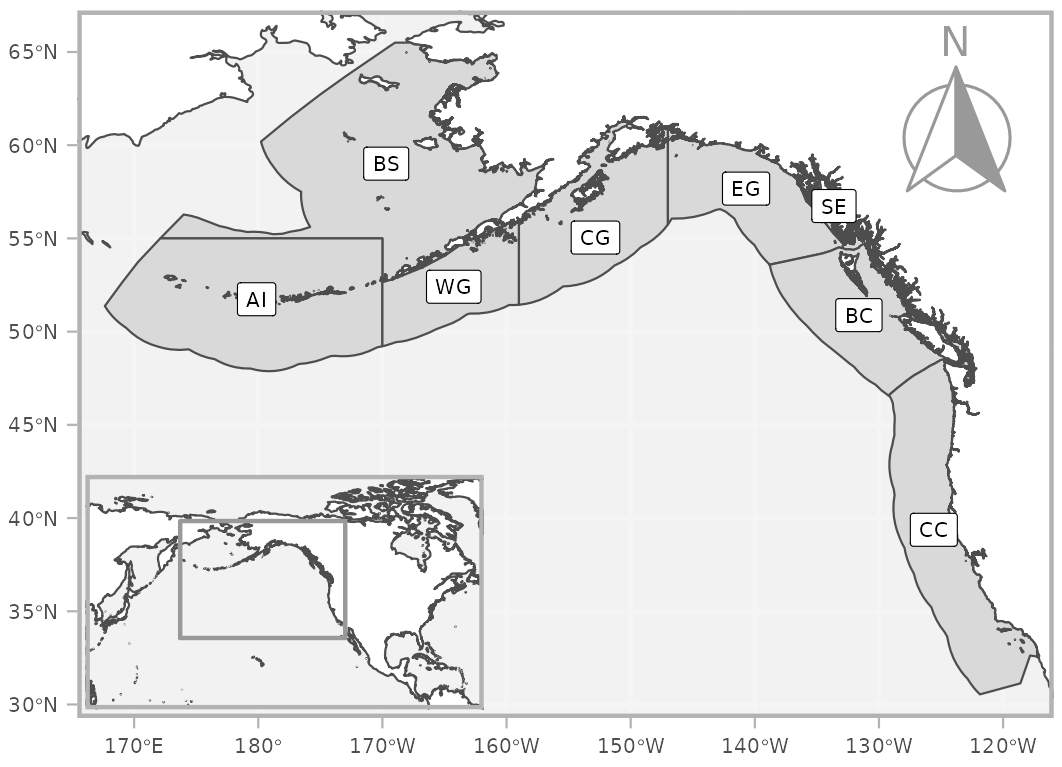
\includegraphics[width = 0.47\textwidth]{map-regions}
    \caption{Geographic sablefish regions in the northeast Pacific Ocean. Regions are Bering Sea (BS), Aleutian Islands (AI), Western (WG), Central (CG), and Eastern Gulf of Alaska (EG), Southeast Alaska (SE), British Columbia (BC), and California Current (CC). Sablefish are managed separately in Alaska (BS--EG), Southeast Alaska, British Columbia, and California Current.}
    \label{fig:map-regions}
\end{figure}

The movement model predicted annual tagged sablefish abundance in each region, and annual numbers of reported recovered tags from each release cohort. Annual survival rates were estimated from harvest, natural mortality, and tag loss rates. Reported tags were predicted using harvest rates and tag reporting rates. Movement rates, harvest rates, negative binomial dispersion, and random walk process errors (annual time-varying model only) were estimated within each model. Sablefish tag releases and recoveries were input as data. Natural mortality, tag reporting, tag loss, and initial tag loss rates were also model inputs. Stock assessment estimates were used as annual means for harvest rate priors. (See \autoref{tab:symbol-definitions}).

\subsection{Questions}
\begin{enumerate}
    \item How much do sablefish move among geographic regions? 
        \begin{itemize}
            \item Model: \texttt{region-average-pooled}
            \item Visual: \autoref{fig:heat-region-average-pooled}
            \item Notes: standard data and priors
        \end{itemize}
    \item How sensitive are sablefish transition rates to alternative reporting rate assumptions?
        \begin{itemize}
            \item Model: \texttt{region-average-pooled}
            \item Visual: \autoref{fig:bar-sensitivity-reporting} (SI)
            \item Notes: six model fits---33\% increase or 50\% decrease for one region in each fit
        \end{itemize}
    \item How sensitive are sablefish transition rates to harvest rate priors?
        \begin{itemize}
            \item Model: \texttt{region-average-pooled}
            \item Visual: TODO scatterplot; one panel per region; retention (and CIs) vs harvest prior sd multiplier (SI)
            \item Notes: five model fits; harvest rate prior sd scaled to mean by progressively wider multiplier
        \end{itemize}    
    \item How much do sablefish transition rates vary by length class?
        \begin{itemize}
            \item Model: \texttt{region-average-length}
            \item Visual: \autoref{fig:heat-region-average-length} (SI)
            \item Notes: standard data and priors
        \end{itemize}    
    \item How much do sablefish transition rates vary by season?
        \begin{itemize}
            \item Model: \texttt{region-season-pooled}
            \item Visual: TODO scatterplot matrix; transition rate (and CI) vs season  
            \item Notes: standard data and priors
        \end{itemize}    
    \item How much do sablefish transition rates vary by year?
        \begin{itemize}
            \item Model: \texttt{region-year-pooled}
            \item Visual: TODO scatterplot matrix; transition rate (and CI) vs year  
            \item Notes: standard data and priors
        \end{itemize}    
    \item How much do sablefish transition rates by length class vary by season?
        \begin{itemize}
            \item Model: \texttt{region-season-length}
            \item Visual: TODO scatterplot matrix; transition rate (and CI) vs season (SI)
            \item Notes: standard data and priors
        \end{itemize}
    \item How many sablefish moved between regions each year?
        \begin{itemize}
            \item Model: \texttt{region-year-length}
            \item Visual: TODO barplot; one panel per border; directional (bars) and net (line) movement
            \item Notes: standard data and priors; abundance at length data (scaled proportional to survey biomass index for Alaska regions)
        \end{itemize}    
    \item What is the relationship between sablefish density and transition rates?
        \begin{itemize}
            \item Model: \texttt{region-year-pooled}
            \item Visual: TBD
            \item Notes: TBD ideally use annual biomass estimates as proxy for relative density
        \end{itemize}    
    \item Does the movement model recover known parameters on simulated data adequately?
        \begin{itemize}
            \item Model: \texttt{region-average-pooled}
            \item Visual: TBD
            \item Notes: TBD
        \end{itemize}
\end{enumerate}

% heat-region-average-pooled
\begin{figure}[htb]
    \centering
    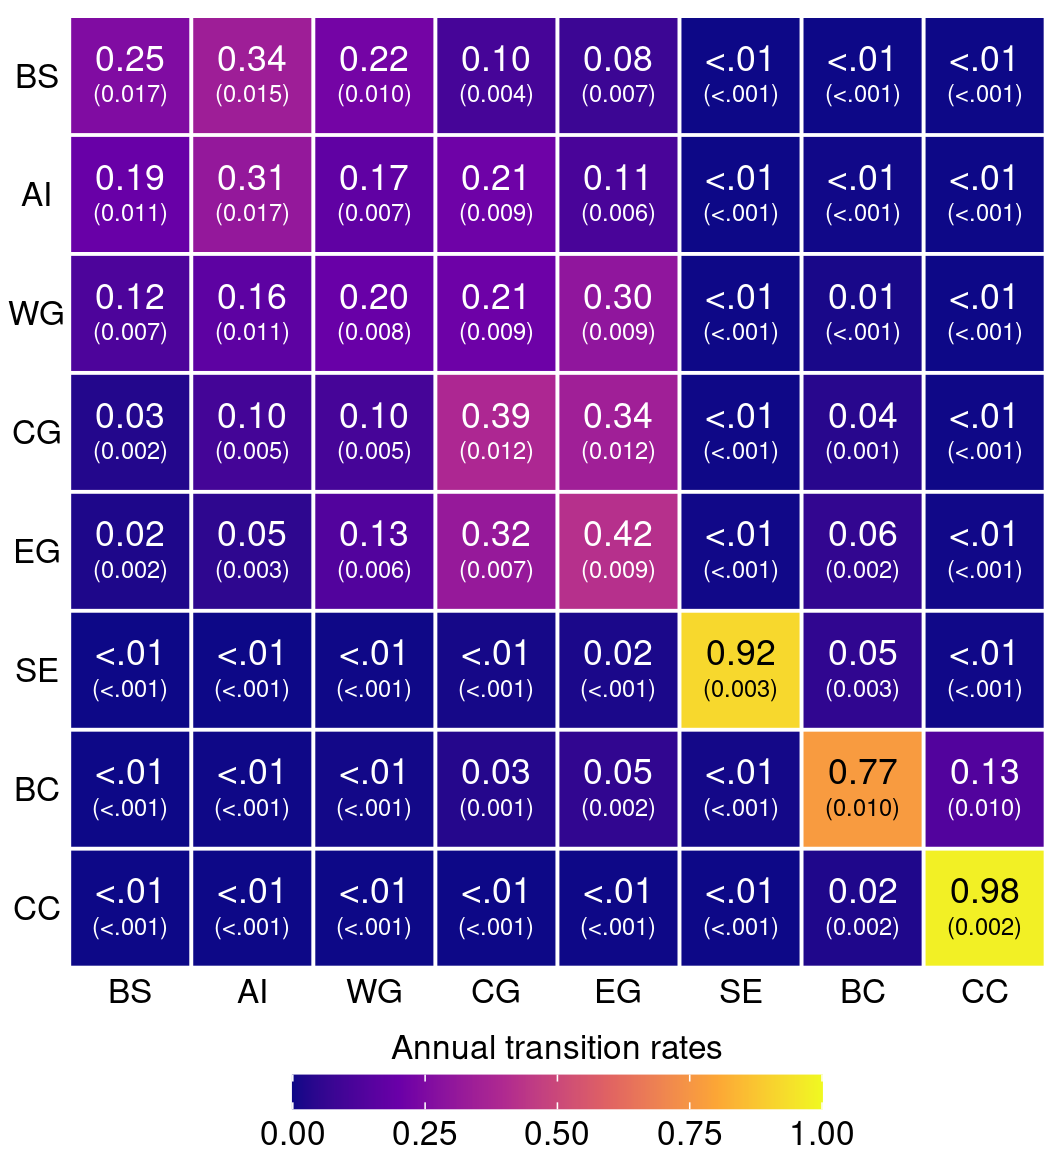
\includegraphics[width = 0.47\textwidth]{heat-region-average-pooled}
    \caption{Sablefish transition rates per year between geographic regions in the northeast Pacific Ocean. The main diagonal shows retention rates while the off-diagonals show emigration rates. Rows correspond to region of origin while columns represent destination. Transition rates are shown with (standard error). Regions are Regions are Bering Sea (BS), Aleutian Islands (AI), Western (WG), Central (CG), and Eastern Gulf of Alaska (EG), Southeast Alaska (SE), British Columbia (BC), and California Current (CC).}
    \label{fig:heat-region-average-pooled}
\end{figure}


\section{Supplementary Information}
% bar-sensitivity-reporting
\begin{figure}[htb]
    \centering
    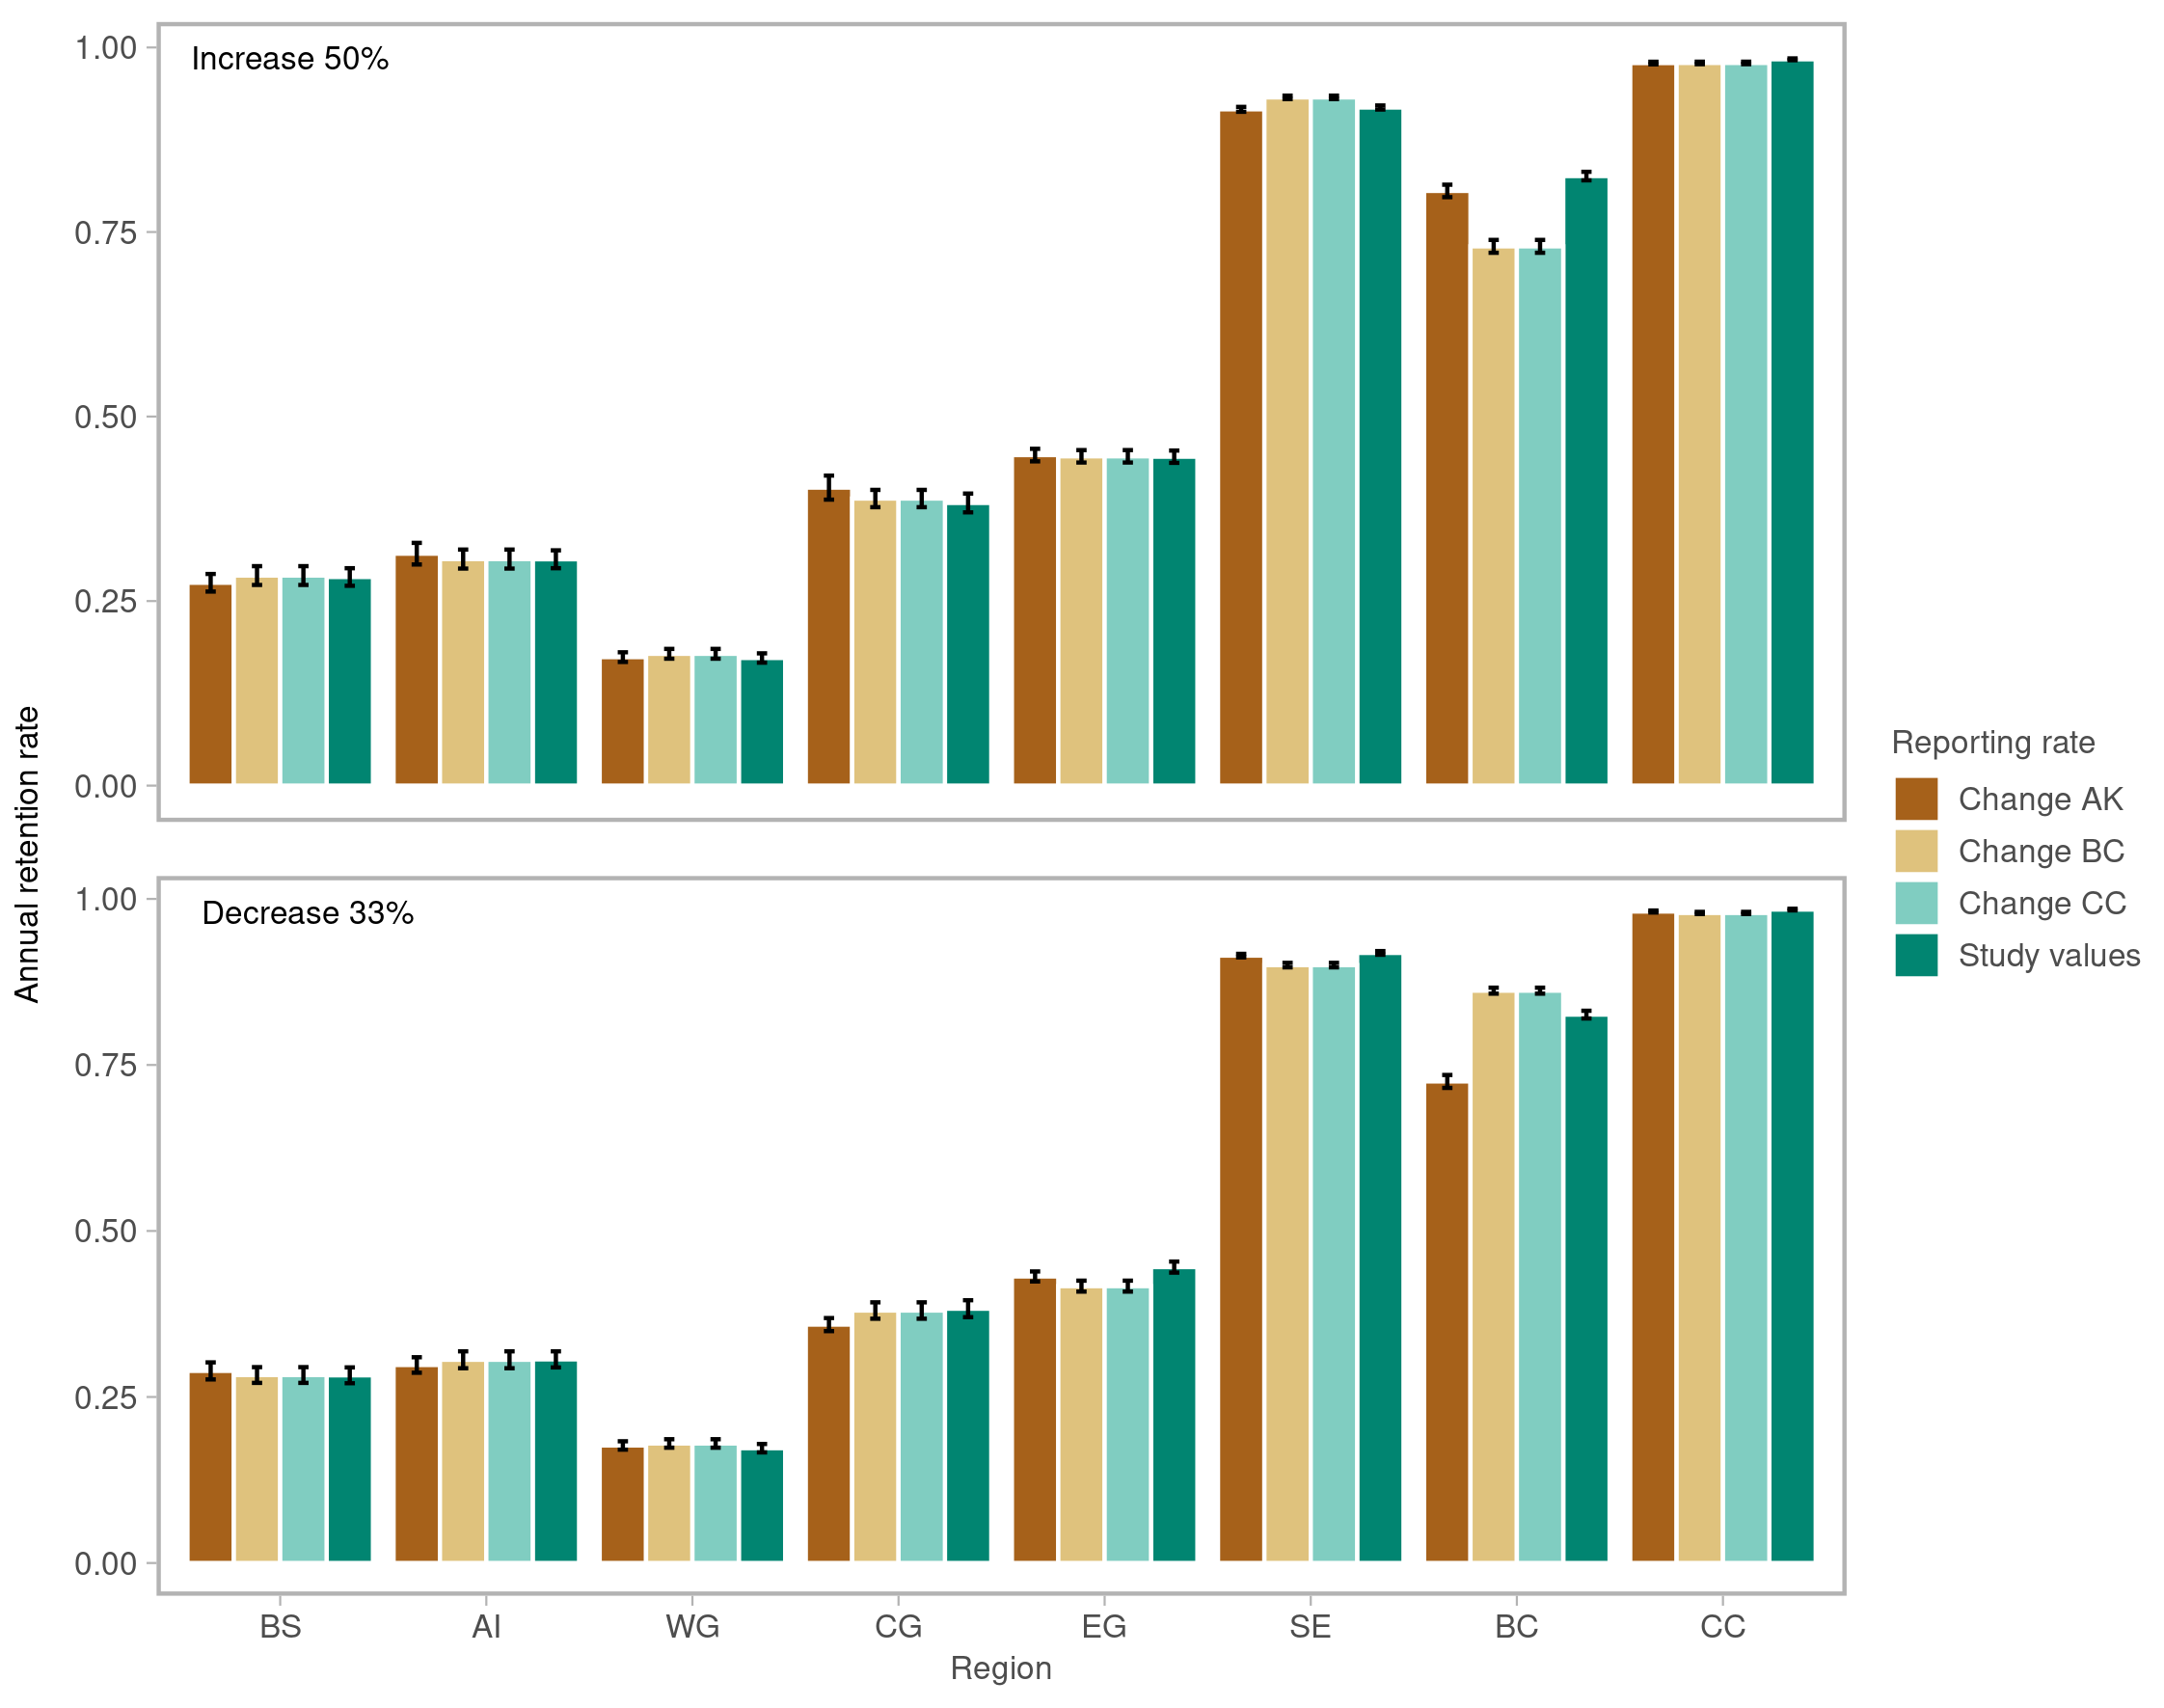
\includegraphics[width = 0.7\textwidth]{bar-sensitivity-reporting}
    \caption{}
    \label{fig:bar-sensitivity-reporting}
\end{figure}

% heat-region-average-length
\begin{figure}[htb]
    \centering
    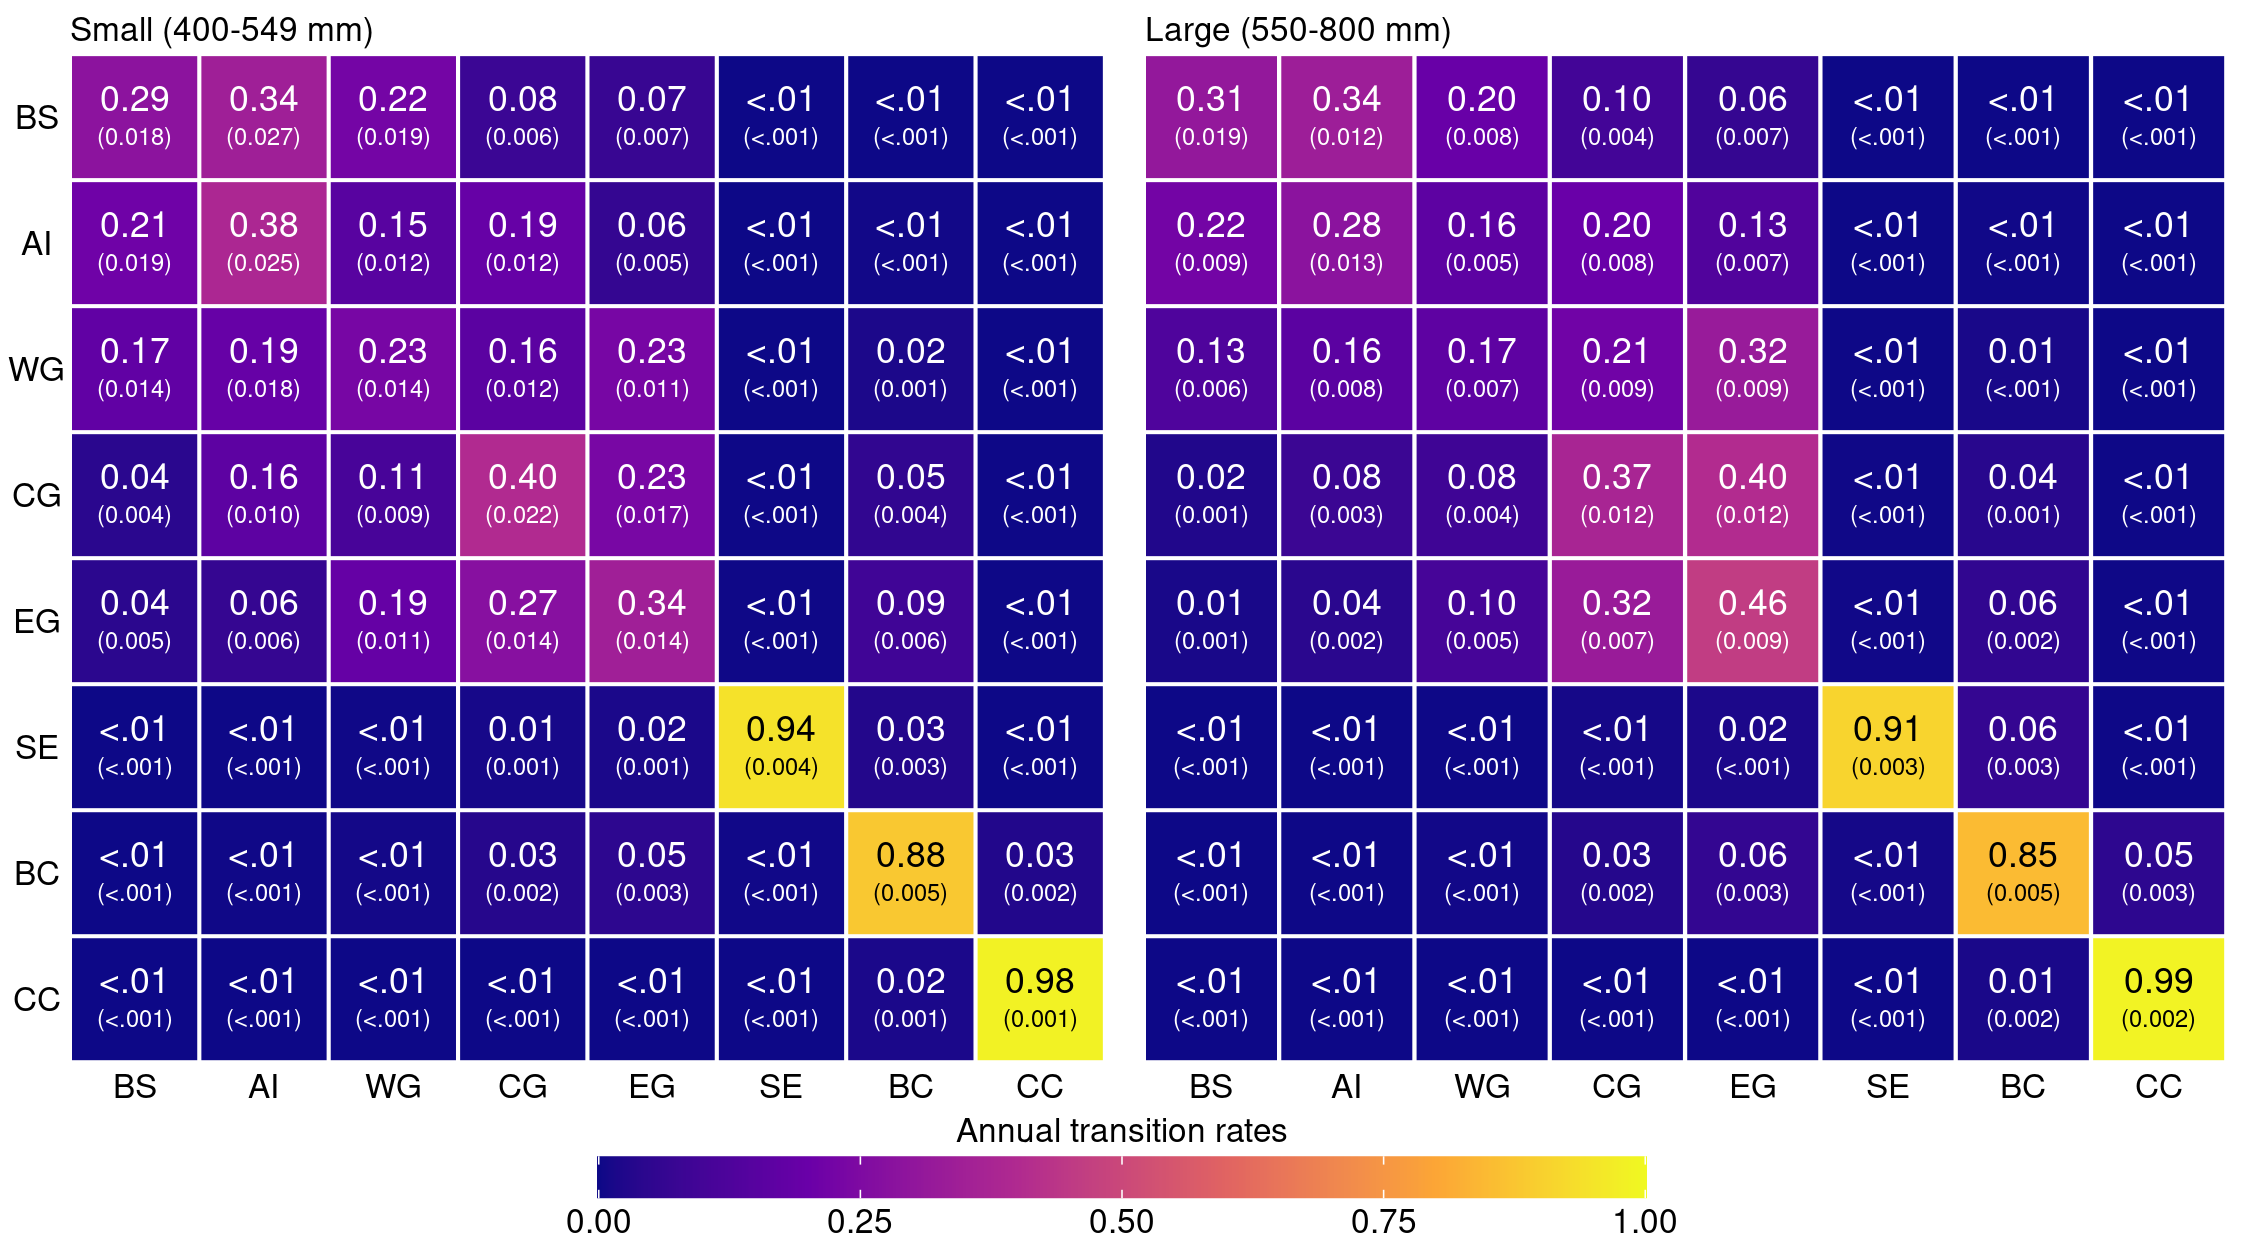
\includegraphics[width = \textwidth]{heat-region-average-length}
    \caption{Sablefish transition rates per year between geographic regions in the northeast Pacific Ocean. Left: small released length class (400--549 mm); Right: large released length class (550--800 mm). The main diagonal shows retention rates while the off-diagonals show emigration rates. Rows correspond to region of origin while columns represent destination. Transition rates are shown with (standard error). Regions are Regions are Bering Sea (BS), Aleutian Islands (AI), Western (WG), Central (CG), and Eastern Gulf of Alaska (EG), Southeast Alaska (SE), British Columbia (BC), and California Current (CC).}
    \label{fig:heat-region-average-length}
\end{figure}

\section{Tables}
% Symbol definitions
\begin{table}[ht]
  \centering
  \caption{Symbol definitions (in progress)}
  \renewcommand\arraystretch{1.2}
  \label{tab:symbol-definitions}
  \begin{tabular}{l l l l r}
    \toprule
    \textbf{Symbol} & \textbf{Condition} & \textbf{Dimension} & \textbf{Definition} & \textbf{Type} \\
    \midrule
    % Index limits
    $A$ & $\in \mathbb{Z}^{+}$ & $\in \mathbb{Z}$ & Number of geographic areas & Index limit \\
    $G_{\mathrm{rel}}$ & $\in \mathbb{Z}^{+}$ & $\in \mathbb{Z}$ & Number of release length groups & Index limit \\
    $G_{\mathrm{harv}}$ & $\in \mathbb{Z}^{+}$ & $\in \mathbb{Z}$ & Number of harvest rate length groups & Index limit \\
    $T_{\mathrm{rel}}$ & $\in \mathbb{Z}^{+}$ & $\in \mathbb{Z}$ & Number of release time steps & Index limit \\
    $T_{\mathrm{lib}}$ & $\in \mathbb{Z}^{+}$ & $\in \mathbb{Z}$ & Maximum at liberty time steps & Index limit \\
    $T_{\mathrm{study}}$ & $\in \mathbb{Z}^{+}$ & $\in \mathbb{Z}$ & Number time steps in the study & Index limit \\
    $T_{\mathrm{mov}}$ & $\in \mathbb{Z}^{+}$ & $\in \mathbb{Z}$ & Number of movement rate time steps & Index limit \\ 
    $T_{\mathrm{harv}}$ & $\in \mathbb{Z}^{+}$ & $\in \mathbb{Z}$ & Number of harvest rate time steps & Index limit \\
    $T_{\mathrm{rep}}$ & $\in \mathbb{Z}^{+}$ & $\in \mathbb{Z}$ & Number of reporting rate time steps & Index limit \\
    $T_{\mathrm{year}}$ & $\in \mathbb{Z}^{+}$ & $\in \mathbb{Z}$ & Number of release time steps per year & Index limit \\
    \midrule
    % Index functions
    $P_T \! \left(\right)$ & $\in \left[1 \, .. \, T_{\mathrm{mov}} \right]$ & $\in \mathbb{Z}$ & $P_T \colon \left[1 \, .. \, T_{\mathrm{study}} \right] \to \left[1 \, .. \, T_{\mathrm{mov}} \right]$ & Index function \\
    $H_T \! \left(\right)$ & $\in \left[1 \, .. \, T_{\mathrm{harv}} \right]$ & $\in \mathbb{Z}$ & $H_T \colon \left[1 \, .. \, T_{\mathrm{study}} \right] \to \left[1 \, .. \, T_{\mathrm{harv}} \right]$ & Index function \\
    $H_G \! \left(\right)$ & $\in \left[1 \, .. \, G_{\mathrm{harv}} \right]$ & $\in \mathbb{Z}$ & $H_G \colon \left[1 \, .. \, G_{\mathrm{rel}} \right] \to \left[1 \, .. \, G_{\mathrm{harv}} \right]$ & Index function \\
    $W_T \! \left(\right)$ & $\in \left[1 \, .. \, T_{\mathrm{rep}} \right]$ & $\in \mathbb{Z}$ & $W_T \colon \left[1 \, .. \, T_{\mathrm{study}} \right] \to \left[1 \, .. \, T_{\mathrm{rep}} \right]$ & Index function \\
    \midrule
    % Index variables
    $a_{\mathrm{rel}}$ & $\in \left[1 \, .. \, A \right]$ & $\in \mathbb{Z}$ & Release area & Index \\
    $a_{\mathrm{prev}}$ & $\in \left[1 \, .. \, A \right]$ & $\in \mathbb{Z}$ & Previous area & Index \\
    $a_{\mathrm{curr}}$ & $\in \left[1 \, .. \, A \right]$ & $\in \mathbb{Z}$ & Current area & Index \\
    $g_{\mathrm{rel}}$ & $\in \left[1 \, .. \, G_{\mathrm{rel}} \right]$ & $\in \mathbb{Z}$ & Release length group & Index \\
    $g_{\mathrm{harv}}$ & $\in \left[1 \, .. \, G_{\mathrm{harv}} \right]$ & $\in \mathbb{Z}$ & Harvest rate length group & Index \\
    $t_{\mathrm{rel}}$ & $\in \left[1 \, .. \, T_{\mathrm{rel}} \right]$ & $\in \mathbb{Z}$ & Release time step & Index \\
    $t_{\mathrm{lib}}$ & $\in \left[1 \, .. \, T_{\mathrm{lib}} \right]$ & $\in \mathbb{Z}$ & At liberty time step & Index \\
    $t_{\mathrm{curr}}$ & $\in \left[1 \, .. \, T_{\mathrm{study}} \right]$ & $\in \mathbb{Z}$ & Current time step & Index \\
    $t_{\mathrm{mov}}$ & $\in \left[1 \, .. \, T_{\mathrm{mov}} \right]$ & $\in \mathbb{Z}$ & Movement rate time step & Index \\
    $t_{\mathrm{rep}}$ & $\in \left[1 \, .. \, T_{\mathrm{rep}} \right]$ & $\in \mathbb{Z}$ & Reporting rate time step & Index \\
    \midrule
    % Input data


    % Predicted values
    % Parameters
    $\bm{p}$ & $\in \left[0, 1 \right]$ & $\in \mathbb{R}^{A \times A \times T_{\mathrm{mov}} \times G_{\mathrm{rel}}}$ & Annual movement rates between areas & Parameters \\
    $\bm{h}$ & $\in \left[0, 1 \right]$ & $\in \mathbb{R}^{G_{\mathrm{harv}} \times T_{\mathrm{harv}} \times A}$ & Annual harvest rates & Parameters \\
    $\phi$ & $\in \mathbb{R}^{+}$ & $\in \mathbb{R}$ & Negative binomial dispersion & Parameters \\
    $\bm{\sigma}$ & $\in \mathbb{R}^{+}$ & $\in \mathbb{R}^{A}$ & Optional random walk standard deviation & Parameters \\
    
    % $s$ & holder & Release Time & Index \\
    % $r$ & holder & Release Area & Index \\
    % $g$ & holder & Release Class & Index \\
    % $t$ & holder & Time & Index \\
    % $a$ & holder & Area & Index \\
    % $i$ & holder & Area & Index \\
    % $T_{s,r,g}$ & holder & Tags Released & Model input \\
    % $R_{s,r,g,t,a}$ & holder & Tags Recovered & Model input \\
    % $F_{t,a}$ & holder & Fishing Mortality Rate & Model input \\
    % $W_{t,a}$ & holder & Tag Reporting Rate & Model input  \\
    % $h$ & holder & Tag Loss Rate & Model input \\
    % $c$ & holder & Initial Tag Loss Rate & Model input  \\
    % $N_{s,r,g,t,a}$ & holder & Tag Abundance & Model output \\
    % $\hat{R}_{s,r,g,t,a}$ & holder & Model output Tags Recovered & Model output \\
    % $S_{t,a}$ & holder & Survival Rate & Model output \\
    % $\Phi_{i,a}$ & holder & Movement Parameters & Model output \\
    % $P_{i,a}$ & holder & Movement Rates & Model output  \\
    % $b_{g}$ & holder & Selectivity and Bias & Model output  \\
    % $M$ & holder & Natural Mortality Rate & Model output  \\
    % $\phi$ & holder & Negative Binomial Dispersion & Model output \\
    \bottomrule
  \end{tabular}
\end{table}




\newpage
\vspace{20mm}

\section{Everything below here subject to extensive revision}

\vspace{20mm}





\section{Overview}
Animal movement rates underlie spatial population dynamics and can influence the effectiveness of management strategies for harvested species. We quantified sablefish movement rates among geographic regions in the northeast Pacific by fitting Markov movement models to forty years of tag--recapture data. The simplest version of our model used three geographic regions (Alaska, British Columbia, and the US West Coast), time-averaged movement rates, and one pooled length class. Additional versions of the model increased the complexity of the model in space (subregional geographic resolution), time (seasonal or annual time-varying movement rates), or length class (small: 40--55 cm; large: 55--80 cm). Models were identified by their geographic resolution (region or subregion), temporal resolution (average, season, or annual), and length class (pooled or length). Movement rates refer to the estimated per sablefish probability of moving from one region to another (emigration rate) or remaining within a region (retention rate) per year.

The movement model predicted annual tagged sablefish abundance in each region, and annual numbers of reported tags from each release cohort. Annual survival rates were estimated from harvest, natural mortality, and tag loss rates. Reported tags were predicted using harvest rates and tag reporting rates. Movement rates, harvest rates, negative binomial dispersion, and random walk process errors (annual time-varying model only) were estimated within each model. Sablefish tag releases and recoveries were input as data. Natural mortality, tag reporting, tag loss, and initial tag loss rates were also treated as data. Stock assessment estimates were used as annual means for harvest rate priors.

\section{Questions}
% - Questions with model formulation bullets
\begin{enumerate}
    \item How much do sablefish movement rates vary between region?
    \begin{itemize}
        \item Model: \texttt{region-average-pooled}
        \item Notes: standard data and priors
        \item Visual: heat  matrix; supplemental information
    \end{itemize}
    \item How sensitive are sablefish movement rates to alternative assumptions about reporting rates?
    \begin{itemize}
        \item Model: \texttt{region-average-pooled}
        \item Notes: three model fits; 50\% increase in tag reporting rate for one region in each fit
        \item Visual: bar plot; one panel per region; retention rate vs region increased; supplemental information
    \end{itemize}
    \item How sensitive are sablefish movement rates to prior information on region specific harvest rates over time?
    \begin{itemize}
        \item Model: \texttt{region-average-pooled}
        \item Notes: five model fits with progressively wider harvest rate priors
        \item Visual: scatter plot; one panel per region; retention (and CIs) vs harvest prior sd; supplemental information
    \end{itemize}
    \item How much do sablefish movement rates vary by length class?
    \begin{itemize}
        \item Model: \texttt{region-average-length}
        \item Notes: standard data and priors
        \item Visual: heat matrix; one panel per length class; main text
    \end{itemize}
    \item How much do sablefish movement rates vary by season?
    \begin{itemize}
        \item Model: \texttt{region-season-pooled}
        \item Notes: standard data and priors
        \item Visual: scatterplot matrix; movement rate (and CIs) vs season; main text
    \end{itemize}
    \item How much do sablefish movement rates vary by year?
    \begin{itemize}
        \item Model: \texttt{region-annual-pooled}
        \item Notes: standard data and priors
        \item Visual: scatterplot matrix; movement rate (and CIs) vs year; main text
    \end{itemize}
    \item How much do sablefish movement rates vary by subregion?
    \begin{itemize}
        \item Model: \texttt{subregion-average-pooled}
        \item Notes: standard data and priors
        \item Visual: heat matrix; one panel; main text
    \end{itemize}
    \item How much do sablefish movement rates among subregions vary by year? (if possible)
    % - Brendan curious
    \begin{itemize}
        \item Model: \texttt{subregion-annual-pooled} (or \texttt{subregion-annual-length})
        \item Notes: standard data and priors
        \item Visual: scatterplot matrix; movement rate (and CIs) vs year; supplemental information
    \end{itemize}
    \item How much do sablefish movement rates by length class vary by season? (if possible)
    \begin{itemize}
        \item Model: \texttt{region-season-length} (or \texttt{subregion-season-length})
        \item Notes: standard data and priors
        \item Visual: scatterplot matrix; movement rate (and CIs) vs year; supplemental information
    \end{itemize}
    \item How many sablefish moved between regions each year?
    \begin{itemize}
        \item Model: \texttt{region-annual-length}
        \item Notes: standard data and priors
        \item Visual: barplot; one panel per border; movement north (upward) and south (downward) and net movement (line)
    \end{itemize}
\end{enumerate}


\section{Figures}
% - Somewhere show priors and posteriors (if interesting) for each estimated parameter in each model
% - Heat matrices: different colour scales for retention (dark mako) and emigration (light rocket)?
% - Spell out panel names: "small", "medium", "large", "pooled", etc.
\subsection{Main text}
\begin{enumerate}
    \item Map: northeast Pacific
    \begin{itemize}
        \item Lines (solid): Regions
        \item Lines (dashed): Subregions
        \item Points (transparent): Sablefish tag releases
    \end{itemize}
    \item Multipanel scatterplot matrix; movement rates (and CIs) vs season or year
    \begin{itemize}
        \item Column 1: \texttt{region-season-pooled}
        \item Column 2: \texttt{region-annual-pooled}
    \end{itemize}
    \item Multipanel heat matrix; movement rates (colour, text) and standard errors (text only)
    \begin{itemize}
        \item Row 1: \texttt{subregion-average-pooled} (single large panel)
        \item Row 2: \texttt{region-average-length} (panels by length class)
    \end{itemize}
    \item Barplot: net abundance exchange vs year
    \begin{itemize}
        \item Row 1: Alaska--British Columbia movement
        \item Row 2: British Columbia--US West Coast movement
        \item Bar direction: upward (north) and downward (south)
        \item Bars: Absolute movement
        \item Points and line: Net movement
        \item Superimposed on map of coast
    \end{itemize}
\end{enumerate}
\subsection{SI}
\begin{enumerate}
    \item Scatter plot: harvest rate priors and posteriors; panels by region
    \item Line plot: tag reporting rate vs year; panels by region
    \item Histogram: sablefish length distributions; length classes superimposed; panels by region
    \item Heat matrix: \texttt{region-average-pooled}
    \item Bar plot: reporting rate sensitivity
    \item Scatter plot: harvest prior sensitivity
    \item Scatter plot matrix: \texttt{subregion-annual-pooled} (if possible)
    \item Scatter plot matrix: \texttt{region-season-length} (if possible)
    \item Line plot: stock assessment abundance vs year; panels by region
    \item Barplot: net abundance exchange vs season
    \begin{itemize}
        \item Row 1: Alaska--British Columbia movement
        \item Row 2: British Columbia--US West Coast movement
        \item Bar direction: upward (north) and downward (south)
        \item Bars: Absolute movement
        \item Points and line: Net movement
    \end{itemize}

\end{enumerate}

\section{Tables}
\begin{enumerate}
    \item Summary of sablefish tag data: numbers, years, sources
    \item Movement model symbol definitions
\end{enumerate}


\newpage
\vspace{20mm}

\section{Everything below here subject to EVEN MORE extensive revision}

\vspace{20mm}



\section{MS layout}
\begin{itemize}
\item Updated versions of sections appear higher up
\item Old versions of sections appear lower down
\end{itemize}


\section{Potential co-authors}

\begin{itemize}
    \item Philina English (Figure design [x], study design [], writing/editing [ ], ...)
    \item Brendan Aulthouse % tag reporting rates
    \item Katelyn Bosley % initial model fits (Juneau)
    \item Meghan Burton % model development
    \item Sean Cox
    \item Katy Echave % tag data
    \item Daniel Goethel % study design
    \item Samuel Johnson % data inputs
    \item Lisa Lacko % tag data
    \item Chris Lunsford
    \item Andre Punt
    \item Cara Rodgveller
    \item Susan Sogard % tag data
    \item Jane Sullivan
    \item Ben Williams
\end{itemize}


% \author[3]{Brendan Aulthouse}
% \author[4]{Katelyn Bosley}
% \author[3]{Meghan Burton}
% \author[3]{Sean Cox}
% \author[6]{Katy Echave}
% \author[6]{Daniel Goethel}
% \author[3]{Samuel Johnson}
% \author[2]{Lisa Lacko}
% \author[6]{Chris Lunsford}
% \author[8]{Andre Punt}
% \author[6]{Cara Rodgveller}
% \author[9]{Susan Sogard}
% \author[10]{Jane Sullivan}
% \author[10]{Ben Williams}
% 
% \affil[2]{Pacific Biological Station, Fisheries and Oceans Canada, Nanaimo, BC, V9T 6N7, Canada}
% \affil[3]{Resource and Environmental Management, Simon Fraser University, Burnaby, BC, V5A 1S6, Canada}
% \affil[4]{Washington Department of Fish and Wildlife, ...}
% \affil[5]{Institute of Ocean Sciences, Fisheries and Oceans Canada, Sidney, BC, V8L 5T5, Canada}
% \affil[6]{Alaska Fisheries Science Center, National Oceanic and Atmospheric Administration,
% Juneau, AK 99801, USA}
% \affil[7]{Northwest Fisheries Science Center, National Oceanic and Atmospheric Administration, Seattle, WA % 98112, USA}
% \affil[8]{School of Aquatic and Fisheries Sciences, University of Washington, Seattle WA 98105, USA}
% \affil[9]{Southwest Fisheries Science Center, National Oceanic and Atmospheric Administration, Santa Cruz, % CA 95060, USA}
% \affil[10]{National Oceanic and Atmospheric Administration, ...}


\subsection{Co-authorship criteria}
Co-authorship and final author order will be based on the PSTAT Data Sharing and Collaboration Agreement (\href{https://docs.google.com/document/d/1AXIhq6lO_qOPf7q67s_SiDOD6qEfih0COtxQZo7v-Hc/edit?usp=sharing}{here}).


\section{Abstract}

\noindent Keywords: 

\section{Introduction}


\section{Methods}
% Movement modeled at end of time step

\subsection{Data}

\subsection{Model}

\subsection{Movement analyses}
% Next steps:
% - Figure script to diagnose fits (posteriors peaked relative to priors)
% - Blocked H by quarter
% - Decide separate or RW movement
% - Sensitivity to reporting rate

% Ways to reduce strain on what the model can do
% - Remove constraint on time at liberty and length buffer
% - Remove US West Coast South (which has very few large sablefish)
% - Use F from previous model fits as strong priors for subsequent
\begin{enumerate}
    \item Static ten subregion pooled
    \begin{itemize}
        \item Full time at liberty
        \item Estimate F (use as prior for length class and restricted time at liberty)
    \end{itemize}
%    \item Static ten subregion length classes
%    \begin{itemize}
%        \item Restricted time at liberty and length buffers
%        \item Use F from pooled as prior (less information to estimate it with data restrictions)
%    \end{itemize}
    \item Static three region pooled (suppress to SI)
    % Gut check on estimating F by comparison to stock assessment estimate
    \begin{itemize}
        \item Full time at liberty
        \item Estimate F (use as prior for length class and restricted time at liberty)
    \end{itemize}    
    \item Static three region length classes (suppress to SI)
    % Brendan: fitting with no constraint on liberty and buffer still worthwhile story acknowledge potential confounding in story
    \begin{itemize}
        \item Restricted time at liberty and length buffers
        \item Use F from pooled as prior (less information to estimate it with data restrictions)
    \end{itemize}
    \item Annual time-varying three region pooled
    \begin{itemize}
        \item Full time at liberty
        \item Estimate F (use as prior for length class and restricted time at liberty)
    \end{itemize} 
%    \item Annual time-varying three region length classes (if possible)
%    % Do ten subregion if everything goes smoothly, but not if poses more difficulties
%    \begin{itemize}
%        \item Restricted time at liberty and length buffers
%        \item Use F from pooled as prior (less information to estimate it with data restrictions)
%    \end{itemize}
    \item Seasonal time-varying three region pooled
    \begin{itemize}
        \item Full time at liberty
        \item Estimate F
    \end{itemize}
%   \item Seasonal time-varying three region length classes (if possible)
%   \begin{itemize}
%       \item Restricted time at liberty and length buffers
%       \item Use F from pooled as prior (less information to estimate it with data restrictions)
%   \end{itemize}
    \item Annual time-varying three region abundance exchange
    \begin{itemize}
        \item Use Annual time-varying three region length classes estimates (if possible)
        \item Use abundance estimates calculated from stock assessments
    \end{itemize}    
\end{enumerate}



\subsection{Sensitivity testing}

\subsection{Model validation}


\section{Results}

\subsection{Movement analyses}

\subsection{Sensitivity testing}

\subsection{Model validation}


\section{Discussion}


\section{Acknowledgements}

\section{References}


\section{Tables}


\section{Figures}


\vspace{20mm}

% TODO
% See Dan Goethel's publications for notation
% Update symbols P Phi W etc in table and equations
% Check capitalization in references
% Change 'movement estimates' and 'movement probabilities' to movement rates
% Replace 'capture rate' by 'fishing mortality rate'
% Replace 'tag reporting ratio' by 'tag reporting rate'
% Specify single release single recapture
% Discuss difference--especially time step--between this and previous models
% Use 'area' in such a way as not to imply 'surface area'; consider 'geographic area'
% Include level of iteration with OM if present
% Description of F weighting equation
% Weight US West Coast catch and PC catch North / South
% Talk with Sue Sogard on WC tag reporting ratio before making a final choice
% Internal review NWFSC: Melissa; AFSC: Kari
% Justification for size classes
% AIC: static, 4 blks, 8 blks
% Time at liberty vs distance travelled cp Beamish and McFarlane
% Discussion: transboundary stock structure, recruitment patterns, spatial population dynamics
% Be sure to reference all tables and figures
% Check that all points in Abstract and Questions are addressed in Results and Discussion
% Release barplot (regions, subregions)
% Replace "reporting rate" by "index of reporting rate"
% Abundance at beginning of time step, movement at end of time step
% Sensitivity of movement rates to harvest priors
% Tags from same release caught together?
% BC: falsify resident/migrant hypothesis? Michelle Jones IBM simulation model proposal
% Simulation testing region-average-pooled
% Novelty
% - Bayesian
% - Estimating h
% - Two spatial resolutions
% - Estimating timevarying p and h

% Notes
% US Fleets are 1: HKL; 2: POT; 3: TWL

% TODO Figures
% Add land for maps
% Releases figure add recoveries panel
% Resize figures and figure components
% Three-subregion movement arrow figure like Meghan's; possibly colour by length
% Three-subregion net exchange arrow figure; movement rates one direction, net movement the other

% TODO Draft
% F for areas within EEZs
% Justification for length classes: show that small ~ immature, medium ~ maturing, large ~ mature via panel figure percent mature over age vs length
% Time-varying movement options

% Main take home messages (for abstract and restate at beginning of discussion)
% - Spatially heterogeneous movement
% - Different movement by length
% - Our estimates of PC movement away are conservative (see sensitivity)
% - Net movement into PC even though larger movement rates away from PC

% Timevarying options
% - Random effect (random walk) for movement parameters on an annual time step
% - Random effect (random walk) for movement parameters on a five or ten year time step
% - Fixed effects blocks for each decade of movement parameters








\section{Abstract}
\noindent 1. We used a Markov movement model fit to \num{\nRelTOT} tag releases and \num{\nRecTOT} tag recoveries over 40 years to estimate the movement of  sablefish among management jurisdictions (i.e, among EEZs) and at finer spatial scales in the northeast Pacific.

\noindent 2. We found that retention rates (average 93 \%) were greater than movement rates (average 7 \%) among EEZs, while retention rates (average 26 \%) were less than movement rates (average 74 \%) for areas within Alaska federal waters. Sablefish movement rates north to Alaska from Pacific Canada North (15 \%) and south to the US West Coast from Pacific Canada South (18 \%) were more than double movement rates between the two Canadian areas (average 7 \%), consistent with a hypothesized north / south separation of sablefish stocks in Pacific Canada. 

\noindent 3. Time-varying movement rates were generally stable across time and length class for Alaska and the US West Coast, but varied widely for Pacific Canada where retention was lowest during 1979--1988 and 2009--2018.

\noindent 4. Despite higher per-fish movement rates out of Pacific Canada, we found that the direction of net abundance exchange was into Pacific Canada from the larger Alaska and the US West Coast populations. Movement rates between Alaska and the US West Coast were less that \num{1} \% either direction.

\noindent 5. Sablefish movement between regions may impact the success of existing management strategies, because fishing rates are set separately in different regions. Further work is needed to investigate the merits of management cooperation among regions such as a coastwide sablefish stock assessment.

\vspace{5mm}
\noindent Keywords: animal movement, movement ecology, mark-recapture, tag-recapture, time-varying movement, transboundary stock,
% release-recapture, capture-recapture

\section{Introduction}

% Consider these to cite:
% First sentence
% Turchin, P. 1998. Quantitative analysis of movement. Sinauer Associates, Inc. Sunderland, MA.
% Williams, B.K., Nichols, J.D, and Conroy, M.J. 2001. Analysis and Management of Animal Populations. Academic Press. San Diego, CA, USA.
% Second sentence
% Cadrin and Secor: https://link.springer.com/chapter/10.1007/978-1-4020-9210-7_22
% Goethel et al: https://www.tandfonline.com/doi/pdf/10.1080/10641262.2011.557451?casa_token=Iqt4--iKgm8AAAAA:XHeP3AtO4tx9RwukqyFIk2Dj3DdzEZk7HXX74CsNhEMnujwRQ9N9FXSejwelTIukYeVzXKRAp-ipLQ

% Why study movement? (Ecology and management perspectives)
Quantifying wildlife movement underpins the study of movement ecology [cite] and the practice of spatial wildlife management [cite]. Animal movement helps shape spatial population dynamics \cite[][]{morales2010} and influences spatial population structure [cite]. [More connecting animal movement to insights about key ecological processes]. As spatial dynamics gain recognition for their role structuring ecosystems [cite], new attention has been given to spatial management and the potential for spatial mismatch between the management actions and the wildlife populations they seek to influence.
\begin{itemize}
\item Do management actions meet wildlife populations at a sensible spatial scale?
\item Benefit of getting it right / pitfalls of getting it wrong % Cite: DG Katelyn B. is developing a manuscript on exactly this topic. Hopefully it will be submitted soonish… Our manuscript on estimating movement in spatial assessment models touches on some of these issues in terms of estimating movement (should be posted to Fish and Fisheries any day now), while Aaron’s paper on the impact of misaligning stock boundaries would also fit here (accepted pending revisions in ICES)….
\end{itemize}
e.g., 
% Perhaps to connect these, a second paragraph should then talk about ‘transboundary’ issues and potential impacts when management domains do not include or misrepresent biological domains/transition zones.  And then move to a paragraph about how to properly detect such domains (i.e., tag data and tagging models; DG: I can see sticking with the tag data theme, but be careful to avoid saying it is best approach...maybe caveat with something like ‘when little genetic variation is observed, tagging data is a useful…’). Then the following paragraph about sablefish makes sense b/c it is a transboundary stock and there is tagging data.

% I think it might be worthwhile to touch on the larger benefit of this work (ie how it can inform transboundary mgmt models).

% DG: We never really touch too much on estimating internal vs. external. My general opinion is that tagging studies are extremely useful to unravel spatial structure and determine the most probable axis of movement (i.e., is it age varying, time varying, diffusive, directional, etc..) and general levels (i.e., does it seem high enough to warrant inclusion in a spatial assessment or are closed populations warranted). If spatial structure and movement seem like important factors influencing population dynamics, then I would encourage the use of a spatial, tag-integrated model, because you are better able to maintain consistency among sub-models and better propagate uncertainty when the tagging data is directly incorporated into the assessment (and maybe help estimate other parameters like M, but you also have to deal with a number of nuisance parameters, tag reporting, etc…, that must be accounted for in the tag model too). I think Kari’s upcoming spatial sablefish assessment manuscript will likely have some discussion of this topic given that she takes the movement parameters from Dana’s tagging model instead of using a tag-integrated assessment. Might be best to cite hers depending on when she submits compared to this paper, etc. Also, given the focus on tagging, it might not be worth getting into the assessment implications in the intro...I was thinking this might make a better discussion paragraph on how these results could be utilized.

\noindent [Transboundary issues]
\begin{itemize}
\item 
\end{itemize}

\noindent [How to detect movement]
\begin{itemize}
\item 
\end{itemize}

% What are the challenges and approaches to studying/quantifying movement?
\noindent Quantifying animal movement can be a challenge in many systems, particularly marine ones.

\begin{itemize}
\item Tags: radio tags for terrestrial animals and birds give sequential locations; acoustic tags for fish can give sequential locations when fish migrate through narrow channels; anchor tags give only the release and recovery locations. % Consider removing. If keep, consider DG if you want to get into tag types, then it is worth noting other types of electronic tags (satellite, PIT), as well as, genetic tags (e.g., close-kin mark recapture) and natural tags (parasite infestation data)
\item Models: Brownie models, hidden Markov models, Hilborn-style models, (earlier approaches summarized in \cite{hilborn1990})
\item Dependence on $F$, reporting rates, selectivity, vulnerability etc. % DG if this is a limitation type paragraph, then also need to consider tag loss, tag mortality, tag mixing, availability, scalability (i.e., do dynamics of a subset of tagged individuals represent the ‘average’ dynamics of the entire population or suite of populations), obtaining adequate sample sizes for releases and recaptures, and potentially difficulties combining disparate tagging data sets
\end{itemize}

% Why study movement in sablefish?
\noindent Sablefish (\textit{Anoplopoma fimbria}) are a commercially valuable groundfish that span three Exclusive Economic Zones (EEZs) in the northeast Pacific and are managed as separate stocks in each jurisdiction despite considerable evidence of population mixing and little genetic evidence of population structure.

\begin{itemize}
\item Sablefish move long distances; long lived; highly valued
\item Population structure from a genetic and movement perspective
\item Geography of sablefish management; transboundary stock
\item Possible consequences of potential spatial mismatch in fishery management
\end{itemize}

% What past work has been done on sablefish movement, what are prevailing hypotheses, what are limitations of this work and unanswered questions?
\noindent Previous work to quantify sablefish movement in the northeast Pacific has focused on tags released in specific EEZs but not coastwide.

\begin{itemize}
\item Sablefish movement originating in Alaska \cite[][]{heifetz1991, maloney2008,hanselman2015}
\item Sablefish movement originating in Pacific Canada \cite[][]{beamish1988,cleary2007}
\item Sablefish movement originating in the US West Coast \cite[][]{sogard2017}
\item Sablefish movement originating in Alaska and the US West Coast \cite[][]{kimura1998}
\item Change in prevailing direction of movement in Alaska \cite[][]{heifetz1991,hanselman2015}
\item Quantification of time-varying movement limited \cite[][]{hanselman2015} (relative strength of retention and movement but not changes in pattern of movement) % DG assuming that this work probably most closely reflects Dana’s paper (I think...still new trying to understand everything that is being modeled, etc..) might be worth highlighting how current work improves on that (i.e., expanding range of study and data sets utilized)....if completely different, then just ignore this comment
\item Separate north and south stocks hypothesis \cite[][]{kimura1998}
\item Hypothesized role of the North Pacific Current Bifurcation \cite[][]{kapur2020}
\end{itemize}

% What questions did we ask?
% DG it might be worth noting the spatiotemporal extent of the tagging data set that we used. I think this is important for setting the stage for the modeling itself, and is interesting just in its unique data richness. 
We analyzed movement originating across all three EEZs in the northeast Pacific, and modelled time-varying changes in movement patterns explicitly. Specifically, we asked (1) How much do sablefish move, measured by individual movement probabilities, among EEZs and areas within EEZs in the northeast Pacific? (2) Does sablefish movement vary by size? (3) Have sablefish movement patterns changed over time? (4) What are the consequences of individual movement for the net exchange of sablefish across EEZ boundaries? and (5) Do patterns of movement support existing hypotheses about northeast Pacific sablefish stock structure and ecosystem features? % DG I usually like to end with a general statement about the potential implications of the study, maybe worth noting that the results will guide development of spatial operating and stock assessment models in the region? Can always just save for the end of discussion, too...

\section{Methods}
% 118: AB: seems like the methods subsections should go 1) Data, 2) Movement Model, 3) Model Validation and so on. This order might reduce some of the repetition I noticed describing and redescribing area and time period definitions as well as help with some definitions introduced in the movement model section (e.g., where F comes from).
% MK I agree with AB on this. MH, I will add my thumbs up to this suggestion; DG, agreed.

% DG Might want to note that this data spans all spatial juridictions, as well.
% AB: ‘abundance exchange” - presumably this is across space over time; maybe “net abundance exchange across defined spatial scales over time”???
We used a Markov movement model and forty years of tagging data to estimate annual sablefish movement rates across the northeast Pacific Ocean. Our goal was to quantify sablefish movement rates and net abundance exchange over time. We estimated movement rates for three release length classes, small (40--55 cm), medium (55--65 cm), and large (65--80 cm); and one pooled length class (40--80 cm). We estimated movement rates separately at two spatial scales: a coarse scale corresponding to the Exclusive Economic Zones (EEZ) for Alaska, Pacific Canada, and the US West Coast; and a finer scale comprising ten areas that partitioned the EEZs (\autoref{fig:map-regions-areas}). The three EEZs were chosen to provide insight into movement among management jurisdictions, while areas within EEZs were chosen to inform movement relative to existing ecological hypotheses. We then paired the estimated movement rates with estimates of sablefish abundance from recent stock assessments to quantify annual sablefish exchange among Alaska, Pacific Canada, and the US West Coast. All data used in our analysis spanned 1979--2018, and were provided by the National Oceanic and Atmospheric Administration (NOAA), Alaska Department of Fish and Game (ADFG), and Fisheries and Oceans Canada (DFO). The data and methods are described in detail in the sections that follow. Data are available at \url{https://github.com/luke-a-rogers/}\lr{\texttt{TBD}}.

\subsection{Movement Model}
% 74: AB: consider “, and a maximum likelihood based objective function.”
% 74: DG: also note that you are estimating annual movement by length class
% 75: I think it is worth mentioning the time step and length based movement assumptions here. I could see moving lines 97-113 to this spot or just summarizing here and going in depth later. Additionally, I find it confusing that none of the equations account for length class. I also am not a big fan of using ‘a’ for area, because it is too easily confused with age, which most population modelers might be expecting.
We developed our movement model following the framework described by \cite{hilborn1990} and adapted for sablefish by \cite{heifetz1991} and \cite{hanselman2015}. The model had three main components: a spatial dynamics model, a tag observation model, and a likelihood function. We estimated annual sablefish movement rates among geographic areas while accounting for unequal fishing mortality rates among areas and length classes.

% 76: DG: maybe note that abundance is indicated by N here. Also, again, movement is by length class so note that here.
% 77: AB: fishing mortality is not typically thought of as an empirical input rate as inferred here though this sentence and Table 2.  It may be worth describing where the fishing mortality rates were taken from (i.e., stock assessments, given this is an outside the assessment or standalone tagging analysis, correct?).
% MH: I agree, some of the F discussion document could be adapted for the methods.
% DG: As I noted in some emails, we are going to need to provide some strong justification for this assumption (I think it is fairly typical to estimate F directly in these types of tag models and fixing F may induce some unknown bias...though parameter correlation is likely to be high if you estimate it, so there is a clear tradeoff) and probably note here that we perform sensitivity runs to the assumed F rates. 

% 78: AB: the bias parameter definition should be described here in detail as it is the first use of it; or point readers to where it is described in more detail (though I didn’t see it described in detail).  So is this bias related to tag mixing, or time of year tags were released, or something else?
%DG: agreed. I’m not sure this is a common approach, so it may need to be thoroughly defined and explained. If there are other tagging models that use this approach, I would suggest citing them for more info on the method.

The spatial dynamics model predicted the abundance of tagged sablefish in each geographic area at each time step. The survival rate $S_{t, a}$ (\autoref{tab:symbol-definitions}) at time $t$ within area $a$ depended on two empirical rates, the fishing mortality rate $F_{t, a}$ for that area and time, and a tag loss rate $h$; and on two model parameters, a selectivity and bias parameter $b_g$ for the release size class, and the natural mortality rate $M$. The survival rate was given by
%
% Survival
\begin{equation}
  \label{eq:survival}
  S_{t,a} = e^{-(b_g F_{t,a} + M + h)}.
\end{equation}
%

% 80: AB: so given all the dynamics occur in area a, then is it safe to presume that movement from area i to area a occurs instantaneously at the beginning of each time step t?  I.e., movement occurs first then population dynamics (survival) occurs for a given time period.
% DG: yea this is important to define explicitly.

%81: AB: ‘movement rates (including retention) that originated in any given area…” - the word originated made me think of the ‘from area i’ meaning of origination?  Is that correct?  Or should it be ‘movement (including retention) rates for each area were…” to be more specific?
% 82 MK I am not totally clear on the difference between movement rates and movement parameters, and the statement re “identified with geographic areas” confused me further. Perhaps open this paragraph defining movement rates vs parameters and how these correspond to geography in plain words, then the mathematical relationship.
% DG: I think you just need to reword that first sentence to more clearly state that the movement rates (i.e., fraction of a population that moves or remains resident) is calculated from the estimated movement parameters using the logit transform to implicitly bound movement between (0,1) and ensure unity in the summation of movement rates. As for the ‘geographic area’ issue, I might suggest adding that the movement rates represent the box-transfer movement probabilities between geographic regions, not the probability of movement for an individual tagged fish based on tag movement histories. Maybe that would reduce confusion a little?
% MH: It would be helpful to add a table to the methods that lists the values used for the fixed model inputs, or just expand table 2.

% Sentence needs a text fix
The movement rates $P_{i, a}$ from area $i$ to area $a$ were derived from the movement parameters $\Phi_{i, a}$ by a multinomial inverse logistic relationship. The movement rates (including retention) that originated in any given area were constrained to sum to one. Because the movement rates were identified with geographic areas rather than for example individual movement histories, the movement model described a Markov process in which geographic areas were Markov states. Because movement probabilities that originated in a given area summed to one, we used one fewer movement than rate parameter for originating area, given by
% 
% 85.5: AB: check the subscripts here as I think the movement rate and movement parameters should be subscript with i and a, not i and j.
% DG: Aaron is right, but I actually prefer i,j rather than i,a as noted in a previous comment regarding the use of a as a subscript.
% 
% 
% Movement rates
\begin{equation}
  \label{eq:movement-rates}
    P_{i,a} = 
    \begin{cases}
      e^{\Phi_{i,a}} \left[1 + \sum_{j \neq i}{e^{\Phi_{i,j}}} \right]^{-1} , &  i \neq a \\
      1 - \sum_{j \neq i}{P_{i,j}}, & i = a.
    \end{cases}
\end{equation} 
%

% 86: DG: I generally prefer to identify a cohort superscript (typically I use lowercase L, for no good reason), which identifies each aspect of a cohort (i.e., release year/time, release area, and release size class), thereby eliminating the need to continually track each of these variables separately. Also, you have now introduced size class g as a subscript, but this was ignored in the mortality and movement terms above. 
The predicted abundance of tagged sablefish $N_{s, r, g, t, a}$ from each release time $s$, release area $r$, and size class $g$, in time $t$ and area $a$ was the number of tag releases $T_{s, r, g}$ after the immediate tag loss rate $c$ was accounted for at the time of release, a prediction of abundance forward in time given local survival and movement after the time of release, and zero before the time of release, as given by
% 
% 89.5: AB: note that equation (1) says St,a where a is the ‘to area’, but in equation (3) for the t>s case it is St-1, i where the i is the ‘from area’.  This brings into question my comment on line 80. I’m sure everything is working as expected in the model, just the nomenclature here may need refining.  Would be good to check all equations for use of i and a.
% DG: definitely agree...I think careful checking of all subscripts, notations, and definitions is warranted. 
% DG: I am guessing that lower case n is the number of regions? This needs to be defined and should probably be in the summation terms in equation 2.
% DG: why is the =0 term needed? When would that apply? Fish can’t go outside the boundaries of the spatiotemporal domain, so I don’t think there is a need for this term. 
% DG: One aspect I am really confused about is how length transitions are accounted for and/or ignored. It seems like the model likely assumes the latter (i.e., estimated parameters/movement apply to the release group regardless of time at liberty). However, it seems like we might be potentially inducing an important bias on length class estimated movement rates, especially if tags are at liberty for any amount of time and/or if a fish is assigned to a length class at the upper bound of that class. In other words, if we assume that size (or size as a proxy of maturity stage) impacts movement, then assuming a fish that was tagged in the small length class, but is at liberty for 5 years (and thus would clearly be in the middle or largest length class by that time), would basically be forcing the model to average movement rates across fish that should no longer be in the same length classes. I have no idea if this is happening or what the bias levels might be (it is probably dependent on the data). I just think we may need to address this assumption at some point (or clarify the description if it is accounted for).
% 
% Predicted abundance
\begin{equation}
  \label{eq:predicted-abundance}
  \begin{aligned}
    N_{s,r,g,t,a} &=
      \begin{cases}
        c T_{s,r,g}, & t = s \text{, } a = r \\
        \sum_{i=1}^n \left( N_{s,r,g,t-1,i} S_{t-1,i} P_{i,a} \right), & t > s \\
        0, & \text{Otherwise.} \\
      \end{cases}
  \end{aligned}
\end{equation} 

% 91: DG: It looks like reporting rate varies by time and region, but it is not estimated. I would suggest noting these here and state where the estimates of reporting rate are derived from.
%92: DG: I would suggest we try to follow the tagging nomenclature in terms of symbols as best we can. I don’t think W for reporting rate is very common. I think lambda and beta are fairly common.
The tag observation model predicted the number of sablefish tags recovered from each area at each time step. We scaled the predicted recoveries by the tag reporting rate because not all recaptured tags were reported. The predicted number of tags recovered $\hat{R}_{s,r,g,t,a}$ depended on the predicted abundance $N_{s,r,g,t,a}$, the tag reporting rate $W_{t, a}$, the fishing mortality rate $F_{t, a}$ and the selectivity and bias parameter $b_g$ as given by

% 93.5: DG: I think this equation is missing a few things, unless I am not understanding the model correctly. Mainly, I don’t think that this recapture equation account for deaths due to natural mortality (occurring continuously throughout the year) or loss of tags (also continuous, I believe). Essentially, the term in parentheses should be 1-Survival multiplied by the fraction of removals from the population due to fishing only. I believe the equation as written would be the recaptures if fishing occurred instantly at the beginning of the year. Maybe that is the assumption we are making? I am probably over thinking it, but it might be good to ensure that we explicitly state the assumptions in terms of timing within a given time step. Also, worth double checking Hoenig 1998 (i.e., Table 2) to ensure equations align with the major assumptions we are using.
% Predicted recoveries
\begin{equation}
  \label{eq:predicted-recoveries}
  \hat{R}_{s,r,g,t,a} = N_{s,r,g,t,a} W_{t,a} \left(1 - e^{-b_g F_{t,a}} \right)
\end{equation}

% 94: AB: note that the ‘movement model’ is a compilation of three components (per lines 73-74), so this sentence is literally saying “The likelihood model evaluated the likelihood … given the spatial dynamics model, the tag observation model, and the likelihood function [i.e., movement model] and data.  Naming is a bit weird here when taken literally.  Nonetheless, I understand it.
% 95: AB: why the subscript 1 for NB?
The likelihood model evaluated the likelihood of a specific set of parameter values given the movement model and data. We used a negative binomial (NB\num{1}) error distribution \cite[similar to][]{hanselman2015} because tagging data typically exhibit overdispersion as a result of non-independence of tagged fish. The likelihood function was defined as \lr{Check}

% 96.5: DG: Don’t think you have defined lowercase phi anywhere

\begin{equation}
  \label{eq:likelihood}
  L\left(\boldsymbol{\Phi}, \boldsymbol{b}, M, \phi \middle| \boldsymbol{T}, \boldsymbol{R}, \boldsymbol{F}, \boldsymbol{W}, h, c \right) = \prod_{s} \prod_{r} \prod_{g} \prod_{t} \prod_{a} \frac{\Gamma \left( \phi \hat{R}_{s,r,g,t,a}^{-1} + R_{s,r,g,t,a} \right)}{\Gamma \left( \phi \hat{R}_{s,r,g,t,a}^{-1} \right) \Gamma \left( 1 + R_{s,r,g,t,a} \right)} \left( \frac{\phi \hat{R}_{s,r,g,t,a}^{-1}}{\phi \hat{R}_{s,r,g,t,a}^{-1} + \hat{R}_{s,r,g,t,a}} \right)^{\phi \hat{R}_{s,r,g,t,a}^{-1}} \left( \frac{\hat{R}_{s,r,g,t,a}}{\phi \hat{R}_{s,r,g,t,a}^{-1} + \hat{R}_{s,r,g,t,a}} \right)^{R_{s,r,g,t,a}}
\end{equation}


We fit the movement model using a monthly time step, and then converted estimates of monthly rates and standard errors to estimates of annual rates and standard errors. Monthly movement rates $P_{i,a}$ were estimated as a matrix $\boldsymbol{P}_{\text{monthly}}$ of pairwise movement rates with retention along the main diagonal. The matrix of monthly movement rates was converted to a matrix of annual movement rates by matrix multiplying $\boldsymbol{P}_{\text{monthly}}$ by itself twelve times, $\boldsymbol{P}_{\text{annual}} = \boldsymbol{P}_{\text{monthly}}^{12}$. We calculated annual movement rate standard errors via bootstrapping. To do this we defined a multivariate normal distribution with vector mean given by the movement parameter estimates, and covariance matrix given by the estimated movement parameter covariance matrix. We then drew 1000 sets of movement parameters from the multivariate normal distribution, and converted each set to a matrix of annual movement rates via \autoref{eq:movement-rates} and the method described above. We then calculated the movement rate standard errors as the sample standard deviation of each annual movement rate across all 1000 draws. We converted the monthly natural mortality rate to an annual rate by   $M_{\text{annual}} = 12 \cdot M_{\text{monthly}}$, because both were instantaneous rates, and we converted the monthly natural mortality rate standard error to an annual standard error via bootstrapping following the same procedure described for movement.

% 108: KF: Consider adding a ‘(Figure 1)’ reference here to remind readers of the area breakdowns. 
% 110: DG: Why are equations 1-2 independent of length class, given that we model length class explicitly? Per earlier comment, what happens when you tag a 55cm fish that is at large for say 5-10 years? Is it always considered a small fish? This could have implications for the results by length class. May need to provide some justification and explicit statements that are/are not modeling transitions among length classes.
% 111: DG: You should probably note that tags were excluded to address incomplete mixing. I would also note that tag mixing is a huge issue and a number of models estimate parameters to address incomplete mixing rates (e.g., scalars on F and/or movement for fish within the ~1st year after release). I wouldn’t be surprised if a reviewer brings up this issue, so it may be worth a sensitivity run or at least being ready to respond with justification for ignoring it.
We fit the movement model to pooled and separated length class data separately for EEZs and areas within EEZs. The pooled length class fits had one release size class (40--80 cm), while the separated length class fits had three release size classes, small (40--55 cm), medium (55--65 cm) and large (65--80 cm), that shared a common error distribution. The selectivity and bias parameter was shared across areas but distinct for each length class. We excluded tags that were recovered in the same time step they were released. We fit the movement model using Template Model Builder (\texttt{TMB}) \cite[][]{kristensen2016} in R (\citeyear{r2020}) via the \texttt{mmmTMB} package (\url{https://github.com/luke-a-rogers/mmmTMB}).


% 114-117: AB: Is it worth here saying why t.v. movement was not looked at using the fine scale areas?  E.g., too many parameters, etc.  And why 4 ten-year periods were chosen?  Seems intuitively parsimonious to me, but others may wonder.
% DG: Yes, justification seems warranted. Also, may be worth noting this earlier when discussing movement. I was under the impression that movement would be fully time-varying as I was reading through the methods.
To estimate time-varying movement rates among EEZs, we fit the model using a distinct set of movement parameters for each ten-year period in one model fit. This gave estimates of movement rates for 1979--1988, 1989--1998, 1999--2008, and 2009--2018. \lr{This is a placeholder for more nuanced time-varying fit ideally using a random effects structure at an annual temporal scale}.

% Integrate to organize as
% Model --> Data --> Reasons for decisions we made --> What we did --> context of previous


\subsection{Data}
% 123:MH: You could add a pers.comm. After ‘EEZ spatial scale’ here from Jane Sullivan, based on the comments in the F document.
% 124: AB: insert ‘the’ after ’areas by’ to emphasize the outside of this study definition of these areas
% 127-128: AB: “...West Coast into two areas at 36…”. “This gave ten total geographic movement areas spanning the 3 EEZs: ….”
% 130-133: AB: solid reasoning -- well done (!), no further questions your honor…
% 132:MH: I would add a reference from the NPFMC in support of the ecosystem breakpoint...
% 124-ish KF: I’m not tracking the numbers and descriptions for AK sub-EEZ regions here. So AK ultimately has six sub-EEZ regions - BS, AI, WG, CG, EG, and SE? I think we’ll need to tweak the language here in a final draft to clarify because for the federal side this set up is fine, but lumps the NPFMC regulatory areas of West Yakuatat, East Yakutat, and Southeast Outside into EG, and then adds SE to account for AK state waters. Some people reading with AK background will see SE and not realize that is state waters. We’ll just want to word smith a bit, I think.
The geographic movement areas used in our analysis were defined at two spatial scales that were analysed separately (\autoref{fig:map-regions-areas}). The EEZs for Alaska, Pacific Canada, and the US West Coast were chosen to represent the broad management jurisdictions at which sablefish are managed as separate stocks. In Alaska, the picture is more complicated. Sablefish stocks in Alaska are managed separately in federal and state areas. We treated Alaska as one movement area for simplicity at the EEZ spatial scale. We used shapefiles from \cite{flanders2018},  edited using the \texttt{sf} package in \texttt{R} \cite[][]{pebezma2018, r2020}, to define the EEZs in our analysis. Within the EEZs, we divided Alaska federal areas by five North Pacific Fishery Management Council (NPFMC) regulatory areas and grouped Alaska state areas including Chatham and Clarence Straits into Southeast Alaska. Pacific Canada was divided in two at \ang{50.5} N, the boundary between Groundfish Management Areas 5A and 3D \cite[][]{sor2007}. We divided the US West Coast in two at \ang{36} N. This gave ten geographic movement areas within the EEZs: Bering Sea (BS), Aleutian Islands (AI), Western Gulf (WG), Central Gulf (CG), and Eastern Gulf (EG), Southeast Alaska (SE), Pacific Canada North (CN), Pacific Canada South (CS), US West Coast North (WN), and US West Coast South (WS). We chose the boundaries at \ang{50.5} N and \ang{36} N to fall near empirical sablefish demographic breakpoints at \ang{50} N and \ang{36} N respectively, while the boundary separating CG and EG at \ang{147} W fell near an ecosystem breakpoint at \ang{145} W  \cite[][]{kapur2020}. The boundary at \ang{50.5} N also fell within the range of seasonal and interannual variability of the North Pacific Current bifurcation \cite[][]{sydeman2011}.

% 139: AB: “inside waters” - maybe change to ‘coastal waters’ to be consistent with wording for Pacific Canada (???)
% 140:MH: Is there a reference for the ADFG tags?
% 142: DG: I feel like an important issue that is completely glossed over here is the appropriateness of aggregating data from multiple, independent tagging programs. I am not certain how common this is and I feel like we need to make some strong justifications here as to why this is appropriate. Again, I am late to the game, so I don’t have a strong background on the data being used. I see in Table 1 that consistent time series are available from all sources. I assume that we cut some of the time series short to have temporal overlap? Also, do all the sources have complete temporal coverage within these years? Do they have consistent spatial coverage within their corresponding geographic release regions across these years? Is there any reason to suspect that tag reporting outside geographic region of release might differ from tags within geographic region of release. I could imagine multiple reasons along these lines including: difficulty tracking down how to report an Alaskan tagged fish caught by a canadian fishermen to scientists in AK/USA and vice versa; limited outreach of tagging programs outside geographic boundaries limiting the interest of fishermen outside the region; fishermen being worried about some type of penalty for catching a fish from another region or thinking there might be long-term consequences for their quota allocations if some crazy scientists tried to start exploring spatial models leading to new allocations, etc.  I am not saying that we shouldn’t combine the data sets, I just think we should discuss why we did it and some of the implications/assumptions associated with that aggregation.
The tagging data included observations of \num{\nRelTOT} sablefish tag releases $T_{s,r,g}$ and \num{\nRecTOT} tag recoveries $R_{s,r,g,t,a}$ from NOAA, ADFG, and DFO (\autoref{tab:tag-data}). Tagged sablefish were released during annual surveys and recovered via surveys and commercial fisheries  (\autoref{fig:map-released-recovered}). Tagged sablefish were released along the continental slopes of Alaska and the US West Coast as part of the National Marine Fisheries Service longline surveys \cite[]{sigler2000, lunsford2014}. An additional \num{17000} tagged sablefish were released off Oregon State during 1996--2004 \cite[described in][]{sogard2017}. In Southeast Alaska, sablefish were tagged and released into inside waters concentrated near Chatham and Clarence Straits. In Pacific Canada, tagged sablefish were released along the continental slope and in four coastal inlets as part of an annual DFO sablefish survey \cite[]{wyeth2007, lacko2020}. We aggregated tagging data into monthly length class specific release and recovery counts for each geographic area. Length classes were defined by fork length upon release, and were small (40--55 cm), medium (55--65 cm) and large (65--80 cm) (\autoref{fig:hist-length-region}), which approximately correspond to immature, maturing, and mature sablefish, respectively. \lr{TODO: show maturity for each EEZ.}

% 146 MK Clarify here the source of Bta -- are these values also from assessments?
% 145-157: AB: how confident are we that the assumptions going into each stock assessment in terms of resulting estimates of F used in this analysis are having little effect on one of the main results of the paper (abstract point 4, net exchange differences).  E.g., fully selected fishing mortality is compiled from each stock assessment/area which themselves have their own selectivity patterns presumably (correct?), and then applied here using a constant (across areas) selectivity and bias parameter. I know there is a F sensitivity, but curious if you thought about this and whether it's worthy of a discussion-based caveat or discussion point.
% DG: agree completely. I think many tagging studies either estimate a combined mortality (Z) component and/or fix M and estimate F. I think all approaches have their caveats, but probably worth noting why we went this route at some point.
% 150-151:MH: We know there are sizable differences in F north and south of 36, so this should be accounted for in the main analysis.
% 152-153: DG: probably worth noting that this was done to better reflect the actual F on on the fully selected ages, which better reflect the tagging data (since a lot of biomass is small fish now).
% 156: DG: Catch in each area or observed tag recaptures? Equation 6 is using tag recaptures not catch.
We approximated fishing mortality rates $F_{t,a}$ from stock assessment estimates of total annual $F$ where available and via estimated harvest rate otherwise. We converted harvest rates to annual instantaneous rates by $F_{t,a} = -\log \left( 1 - C_{t,a} / B_{t,a} \right)$ where $C_{t,a}$ was annual catch and $B_{t,a}$ was annual biomass in a given area. For Alaska, we used estimates of total annual fully-selected $F_t$ for Alaska Federal waters \cite[]{hanselman2019}. For Pacific Canada, we used the estimated annual legal catch and biomass from the BC sablefish stock assessment \cite[][]{dfo2020}. For the US West Coast, we used estimates of total annual fully-selected $F_t$ \cite[]{haltuch2019} (\autoref{fig:line-capture-rate}). We approximated $F_{t,a}$ at a finer spatial scale for areas within Alaska, but continued to use the respective total estimates for areas within Pacific Canada and the US West Coast. For areas within Alaska Federal waters, we used estimates of catch at age four plus by area, and relative population weight by area divided by catchability for biomass \cite[described in][]{hanselman2015}. For Alaska State waters, we used the fully-selected instantaneous fishing mortality rate for Chatham Strait \lr{TODO: Citation}. We converted annual instantaneous fishing mortality rates to the monthly instantaneous rates used in our analysis by weighting the annual rate by the monthly proportion of catch in each area. The monthly instantaneous rates were given by \lr{Resolve time index}
%
% monthly-fishing
\begin{equation}
  \label{eq:monthly-fishing}
  F_{y,m,a}^{\text{monthly}} = \left( \frac{\sum_s \sum_r \sum_g R_{s,r,g,m,a}}{\sum_s \sum_r \sum_g \sum_m R_{s,r,g,m,a}} \right) F_{y,a}^{\text{annual}}
\end{equation}
%
We allowed the weighting to differ by area $a$, but held the weighting constant across years $y$ within an area. We used the proportion of tags recovered by month $m$ as a proxy for the proportion of catch by month. To reduce potential bias from clustered release dates, we used only tag recoveries that were at liberty for one year or more before recapture for the weighting. We calculated weights for Alaska, Pacific Canada and the US West Coast (\autoref{fig:bar-capture-scale-region}) and for areas within the EEZs (\autoref{fig:bar-capture-scale-area}).

We approximated sablefish tag reporting rates using empirical estimates where possible for Alaska, Pacific Canada, and the US West Coast. The tag reporting rate represents the proportion of tagged sablefish that were reported out of the total number recaptured (\autoref{fig:line-report-ratio}). For Alaska, we used the reporting rate estimates for Alaska federal waters \num{0.135}--\num{0.565} from \cite{hanselman2015}, who compared tag returns from the commercial fishery to tag returns from surveys binned to three year intervals \cite[][]{heifetz2001}. For Pacific Canada, we used the mean reporting rate \num{0.550} estimated by comparing commercial and survey tag returns during 2003--2018 \cite[][]{aulthouse2020}. For the US West Coast, we chose a mean reporting rate of \num{0.300} that was lower than for Pacific Canada to reflect lower reporting rates from trawl fisheries which account for a greater portion of the commercial catch from the US West Coast relative to Pacific Canada. 

We assumed an annual instantaneous tag loss rate  of \num{0.02}, and an immediate tag loss rate (i.e., initial proportion of tags lost upon release) of \num{0.1}. These values were estimated from an experiment in which \num{5000} double-tagged sablefish were released in Pacific Canada \cite[][]{saunders1990}.

\subsection{Model Validation}
% 173: DG: Not sure if this section is complete or not, but it seems to kind of gloss over the details of the simulation study, mainly what was assumed about observation error? Also, were any sensitivity runs performed in the simulation to see what bias might be expected to issues like mis-specifying F or reporting rate?
We tested whether the movement model could recover known parameter values by fitting the model repeatedly to simulated data. We simulated tag recovery data from tag releases; fishing, tag reporting, and tag loss rates; and parameter estimates for the pooled release length class at the three EEZ geographic scale. To test our implementation of the movement model in \texttt{TMB}, we coded the tag recovery simulation entirely in R \cite[][]{r2020}. This ensured that a successful recovery of the simulation parameter values by the movement model would indicate both that independent implementations of the model concurred, and that the model could recover known parameter values. We simulated 100 tag recovery data sets. We then compared parameter estimates for movement retention and natural mortality to the known simulation parameters.

\subsection{Sensitivity Analysis}
We tested the sensitivity of annual retention rates to changes in tag reporting and fishing mortality rates by systematically changing these input in repeated fits of the movement model. We used the mean of the input time series or multiplied the time series by \num{1.5} separately for each area. We used the pooled release length class and three EEZs. We recorded the absolute and relative change in annual retention rate for each area under each of these changes to the fishing mortality rate and tag reporting rate (\autoref{fig:bar-sensitivity}).

\subsection{Abundance Exchange}
% 187:MH: You discuss abundance in this section, I usually think in biomass or numbers, it would be good to define what you are specifically referring to, and the units of abundance. 
To quantify the consequences of movement for sablefish abundance in each EEZ, we calculated abundance exchange between Alaska and Pacific Canada, and between Pacific Canada and the US West Coast using estimated movement rates and stock assessment estimates of annual abundance for each EEZ. For Alaska, we summed estimates of abundance-at-length across federal and state waters. For federal waters, we used estimates of abundance-at-age and length-at-age to calculate abundance-at-length \lr{Cite}. For state waters we used abundance-at-length for Chatham Strait \lr{Cite}. For Pacific Canada, we used estimates of abundance-at-age and length-at-age from the sablefish stock assessment for British Columbia to calculate abundance-at-length \cite[]{dfo2020}. For the US West Coast, we used abundance-at-length estimates directly from the stock assessment \cite[]{haltuch2019}. We used the widest range of lengths common to all three EEZs, which was \num{41}--\num{67} cm for males and \num{41}--\num{71} cm for females. Sablefish that moved between Alaska and the US West Coast were assumed to move through Pacific Canada. For example, abundance that moved from Alaska to the US West Coast was included in our estimate of abundance that moved from Alaska to Pacific Canada, and also in our estimate of abundance that moved from Pacific Canada to the US West Coast. This would bias the estimate of exchange high in the sense that some of the inferred exchange was not retained, but rates were less than 1 \% so the effect was negligible.

\section{Results}
% Include movement by sex to descriptive stats
% 204-207: AB: indicating a generally opposite trend compared to many other species, or at least generalized movement theory for fish that the older/larger you get the further you can move.  So Sablefish movement isn’t strictly related to the physics of larger fish tail beats enabling them to move further than smaller fish, but clearly has some habitat competition based movement (or similar).  Interesting.
% KF: though what does this mean in light of Dan’s comments about fish in one release group moving into another size class group while at large? Would those fish be biasing the distance traveled for the small size group?
% 204: MH: add ‘a mean’ before 384.4; same comment for the next sentence so it is clear that you are reporting means.
Sablefish moved long distances. We measured great circle distances between release and recovery, which give conservative estimates of distance travelled. Sablefish moved a mean \num{\dmuTOTapYR} kms (\num{\dqlTOTapYR}, \num{\dquTOTapYR}; \num{2.5} and \num{97.5} \% quantiles, respectively) within the first year following release, and  \num{\dmuTOTapALL} (\num{\dqlTOTapALL}, \num{\dquTOTapALL}) km across all forty years of the study. Sablefish in the small length class moved \num{\dmuTOTasYR} (\num{\dqlTOTasYR}, \num{\dquTOTasYR}) km and \num{\dmuTOTasALL} (\num{\dqlTOTasALL}, \num{\dquTOTasALL}) km over all years. Sablefish in the medium length class moved \num{\dmuTOTamYR} (\num{\dqlTOTamYR}, \num{\dquTOTamYR}) km and \num{\dmuTOTamALL} (\num{\dqlTOTamALL}, \num{\dquTOTamALL}) km over all years. Sablefish in the large length class moved \num{\dmuTOTalYR} (\num{\dqlTOTalYR}, \num{\dquTOTasYR}) km and \num{\dmuTOTalALL} (\num{\dqlTOTalALL}, \num{\dquTOTalALL}) km over all years.

%All movement model fits satisfied our convergence criterion: a positive definite Hessian matrix, and a maximum gradient component $\leq \num{0.00001}$. We report movement rates as the mean estimate $\pm$ the standard error. Because movement rates are on a per fish basis, movement rates originating in the same area are comparable, but rates originating in different areas are not comparable in terms of total movement of fish. We call a movement rate a retention rate when the origin and terminus are the same area.

\subsection{Movement Rates}
% 209 LR Report movement rates as percent (e.g. 24 %) or decimal (e.g. 0.24) but not both.
% 209-211:MH: Why are the standard deviations so small on these estimates? 
% DG: agreed, seems really precise...
% 213: AB: what does AIC say about this statement?  Should length class be a factor?  Or does this statement just reflect ‘on average’? DG: Or is this an issue of not accounting for transition among length classes?
For Alaska, Pacific Canada, and the US West Coast, retention rates were higher than movement rates away from each EEZ (\autoref{fig:heat-movement-03a-static}). Pacific Canada had the lowest retention rate \num{0.86} $\pm$ \num{0.002}  for the pooled length class, while the US West Coast had the highest \num{0.97} $\pm$ \num{0.002}. The movement rate northward from Pacific Canada \num{0.09} $\pm$ \num{0.002}  was greater than the movement rate southward \num{0.05} $\pm$ \num{0.001} . We found negligible evidence of movement between Alaska and the US West Coast. Movement rates by length class were qualitatively similar to movement rates for the pooled length class. However, for the small length class (\num{40}--\num{55} cm) in Pacific Canada, the retention rate was lower \num{0.82} $\pm$ \num{0.004}  and the northward movement rate was higher \num{0.14} $\pm$ \num{0.004}  than for the pooled length class.

% 221-222: AB: it would be worth describing that this statement is based on AIC 
Time-varying movement rates were generally consistent across time and length class for Alaska and the US West Coast, but varied widely for Pacific Canada (\autoref{fig:line-movement-03a-size-sml-timevary}). Retention rates in Pacific Canada were highest during the two decades 1989--2008 for all three length classes, and lowest during 1979--1988 and 2009--2018. Movement northward from Pacific Canada was highest during 1979--1988, while movement southward was highest during 2009--2018. The small length class (\num{40}--\num{55} cm) showed elevated movement northward from Pacific Canada relative to the medium (\num{55}--\num{65} cm) and large (\num{65}--\num{80} cm) length classes during 1979--1988. The time-varying model received more support from the data than the time-averaged model (\autoref{tab:model-aic}).

% 223: DG: Are all the areas generally the same size? I.e., would we expect the retention to be lower in Alaska because the areas are smaller (not sure they are, but there are more areas within AK than elsewhere, so maybe?)? Also, could these be a factor of lack of reporting of tags from outside geographic regions (i.e., AK fishermen are more likely to report tags from AK tagging studies than tagging studies in CAN or West Coast).
For areas within the EEZs, movement among areas in Alaska federal areas (BS, AI, WG, CG, EG) was qualitatively different from movement among all other areas (SE, CN, CS, WN, WS) (\autoref{fig:heat-movement-10a-static}). Retention rates were lower than cumulative movement rates away from each area in Alaska federal areas, ranging from \num{0.14} $\pm$ \num{0.003}  in the Western Gulf to  \num{0.35} $\pm$ \num{0.024}  in the Bering Sea. By contrast, retention rates were higher than cumulative movement rates away from each area in Southeast Alaska, and within areas in Pacific Canada and the US West Coast, all above \num{0.70}. Sablefish in Pacific Canada North (CN) were twice as likely to move northward \num{0.15} $\pm$ \lr{se}  to Alaska as they were to move southward to Pacific Canada South (CS) or the US West Coast \num{0.07} $\pm$ \lr{se} . Conversely, sablefish in Pacific Canada South were \num{2.25} times more likely to move southward \num{0.18} $\pm$ \lr{se}  than northward \num{0.08} $\pm$ \lr{se} .

Movement rates by length class were qualitatively similar to movement rates for the pooled length class. However, for the small length class (\num{40}--\num{55} cm) in Pacific Canada North, the retention rate was lower \num{0.66} $\pm$ \num{0.009}  and the northward movement rate was twice as high \num{0.28} $\pm$ \lr{se}  as for the pooled length class. There were low rates of movement from Southeast Alaska (SE) to Alaska federal areas \num{0.03} $\pm$ \lr{se}  and negligible movement from Alaska federal areas to Southeast Alaska. Among the Alaska federal areas, there were greater movement rates eastward than westward for the Western and Central Gulf.

\lr{Describe model fits and remaining parameter estimates (Tables 3--6) plus mgc and convergence criteria}

\subsection{Model Validation}

\lr{TBD}

\subsection{Sensitivity Analysis}

% 243: DG: Is this the most realistic alternate F assumption? Just wondering if this might be refined to choose an alternate F by region based on expert opinion? I’m not sure it matters, because I think F and movement are going to be correlated to some extent such that if you included movement in the assessments, the Fs would change, too. Not sure that change would be predictable.
Our sensitivity analysis showed that retention rates for the three EEZs were generally robust to systematic changes in the fishing mortality and tag reporting rates (\autoref{fig:bar-sensitivity}). Replacing the time series of fishing mortality rates for any EEZ by its mean value resulted in absolute and relative changes to the retention rate for all EEZs of $\leq$ \num{0.02} $\pm$ \lr{se} . Multiplying the time series of fishing mortality rates by \num{1.5} for a given EEZ generally decreased the estimated retention rate for that EEZ, and increased the retention rate for the other two EEZs. The largest changes in annual retention rate across increased fishing mortality rate in all three EEZs were seen in Pacific Canada, while in the US West Coast changes in retention rate were negligible. Increasing the time series of fishing mortality rate by a factor of \num{1.5} in Alaska and the US West Coast let to increased estimates of annual retention rate in Pacific Canada by \num{1.8} $\pm$ \num{0.3} \% and \num{1.3} $\pm$ \num{0.3} \%, respectively. Increasing the fishing mortality rate in Pacific Canada led to a decreased in the estimate of annual retention rate in Pacific Canada by \num{4.8} $\pm$ \num{0.4} \%. Changes to the tag reporting rate showed a similar pattern. Increasing the time series of tag reporting rate by a factor of \num{1.5} in Alaska and the US West Coast let to increased estimates of annual retention rate in Pacific Canada by \num{2.5} $\pm$ \num{0.3} \% and \num{1.3} $\pm$ \num{0.3} \%, respectively. Increasing the tag reporting rate in Pacific Canada led to a decreased in the estimate of annual retention rate in Pacific Canada by \num{6.4} $\pm$ \num{0.4} \%.

\subsection{Abundance Exchange}

% 255: DG: Is there any evidence of this source-sink dynamic from the catch data or general dynamics throughout the region? Could this result occur if Canadians just report more tags, because they are friendlier than Americans! I would almost be interested to see if we could develop a simulation scenario that had separate reporting rates based on the combination of geographic location of tagging and recapture (instead of just recapture location) and if we could manipulate movement estimates based only on changing the true/assumed reporting rates….just thinking out loud….
% KF: can we do this and give it a title like “Are Canadians really nicer? What we learned about tag reporting rates via simulation.” (joking...mostly)
The abundance of sablefish moving into Pacific Canada from Alaska and the US West Coast was estimated to exceed the abundance of sablefish moving out of Pacific Canada (\autoref{fig:bar-abundance-exchange-pool-sml}). Despite higher movement rates on a per fish basis out of Pacific Canada, the greater abundance of sablefish in the adjacent EEZs meant more sablefish entered Pacific Canada, even though at a slower per fish rate.
% Fix truncation issue in figure


\section{Discussion}

\noindent We found that 
\begin{itemize}
\item Retention rates were higher than movement rates among EEZs
% 261-262: AB: consistent with previous AK federal waters analyses?
\item Retention rates were lower than movement rates among areas within Alaska federal waters, but not in Pacific Canada or the US West Coast
\item Movement rates north from Pacific Canada North and south from Pacific Canada South were double movement rates between the two areas.
\item Movement rates were relatively stable across time in Alaska and the US West Coast, but varied in Pacific Canada
\item The direction of net abundance exchange was into Pacific Canada from Alaska and the US West Coast despite higher per-fish movement rates out of Pacific Canada
\end{itemize}

\noindent The ecological implications of our key findings for existing hypotheses about
\begin{itemize}
\item Stock structure (Conventional wisdom about stock structure: two stocks with some exchange in BC?) Also North Pacific Current (is movement related to location and intensity of current?)
\item Size-dependent movement (is movement inversely related to spawning biomass a-la Hanselmen 2015?)
\item Note: (a) This works picks up right around a regime shift in the NPO, (b) Interannual swinging of N Pac Current bifurcation
\item Movement east vs movement west
\item Finding that movement > retention in AK but not southern regions. Would be good to speculate why this might be: more shelf habitat, or currents, or ...?
\end{itemize}


\noindent The implications of our key findings for sablefish management
\begin{itemize}
\item Extent of spatial mismatch and potential consequences
\item MH For the mgmt question, most lit examines the situation where movement occurs @ one class and otherwise sedentary (or below a certain threshold) -- worthwhile to qualify where our findings line up along that spectrum.
\end{itemize}

\noindent How much do sablefish move relative to other demersal fish species
\begin{itemize}
\item Hanselman et al. 2015 
\item Hannan and Rankin 2011
\end{itemize}

\noindent What needs to be done to evaluate the consequences of abundance exchange for fisheries management?
\begin{itemize}
\item Distill consequences of ignoring movement.
\item Set the stage for Maia's work on empirically parameterized closed loop simulations to evaluate consequences of ignoring movement
\end{itemize}

% 288: DG:probably the tag reporting and F assumptions need to be discussed. Also, pros/cons of aggregating across independent tagging studies.
\noindent Why did we make the modelling decisions we made / how does this work add to past efforts
\begin{itemize}
\item Monthly time step cp. Hanselman, Heifetz, Hilborn
\item Timevarying cp. Hanselman
\item What other types of tag movement models are out there? Strengths / weaknesses?
\item Can we estimate $Z$ as suggested by Hilborn?
\end{itemize}

% 293: DG: same as above. Limitations due to (lack of) size transition assumptions among size classes. Might bias the size-specific movement rates. Tag mixing assumptions. Scaleability issues (i.e., from individual to representation of the ‘entire’ population/region).
\noindent Limitations of our analysis include
\begin{itemize}
\item MH Consider highlighting the challenge of disentangling movement and spatially varying recruitment, especially with modeled areas of distinct sizes \cite[][]{cadrin2019}. 
\item Model inputs assume no movement (e.g. F)
\item Differences in the size of the geographic areas
\end{itemize}

% 298: DG: Probably need to discuss the implications for assessment. As noted in intro comment, might be worth noting pros/cons of externally estimated movement compared to tag-integrated models (probably cite Kari’s sablefish spatial assessment model).
\noindent What are some next steps and conclusions
\begin{itemize}
\item MH I also see an interesting next step examining the recruitment vs movement question coming out of the climate synthesis led by Melissa. 
\item BC Yes, And perhaps deeper dive into environmental correlates of movement
\item Key unanswered questions
\end{itemize}

\section{Acknowledgements}
\begin{itemize}
\item Funding
\item Data
\item Feedback other than authors
\end{itemize}

\newpage
\bibliography{refs/refs}

% \newpage
% \hypertarget{supp-info}{}
% \section{Supplementary Information}


\newpage
\section{Tables}
% Add a table with mgc for the model fits

% Table of tag data
\begin{table}[ht]
  \centering
  \caption{Sablefish tag data sources}
  \renewcommand\arraystretch{1.2}
  \label{tab:tag-data}
  \begin{tabular}{lrrll}
    \toprule
    \textbf{Locations} & \textbf{Released} & \textbf{Recovered} & \textbf{Years} & \textbf{Source} \\
    \midrule
    Alaska Federal & \num{\nRelAK} & \num{\nRecAK} & 1979--2018 & NOAA \\
    Alaska State & \num{\nRelSE} & \num{\nRecSE} & 1979--2018 & ADFG \\
    Pacific Canada & \num{\nRelBC} & \num{\nRecBC} & 1979--2018 & DFO \\
    US West Coast & \num{\nRelUS} & \num{\nRecUS} & 1979--2018 & NOAA \\
    \bottomrule
  \end{tabular}
\end{table}


% Table 2: AB: Why again is Pi,a included as estimated here? After reading more, is it because it is monthly, where phi is annual?
% DG: I think P should be either a ‘predicted’ value, but I think more accurately it should be a ‘derived’ parameter (based on uppercase phi). Could maybe just replace the whole class of ‘predicted’ values with ‘derived’ values.

% Symbol definitions
\begin{table}[ht]
  \centering
  \caption{Movement model symbol definitions}
  \renewcommand\arraystretch{1.2}
  \label{tab:symbol-definitions-1}
  \begin{tabular}{l l r}
    \toprule
    \textbf{Symbol} & \textbf{Definition} & \textbf{Type} \\
    \midrule
    $s$ & Release Time & Index \\
    $r$ & Release Area & Index \\
    $g$ & Release Class & Index \\
    $t$ & Time & Index \\
    $a$ & Area & Index \\
    $i$ & Area & Index \\
    $T_{s,r,g}$ & Tags Released & Model Input \\
    $R_{s,r,g,t,a}$ & Tags Recovered & Model Input \\
    $F_{t,a}$ & Fishing Mortality Rate & Model Input \\
    $W_{t,a}$ & Tag Reporting Rate & Model Input  \\
    $h$ & Tag Loss Rate & Model Input \\
    $c$ & Initial Tag Loss Rate & Model Input  \\
    $N_{s,r,g,t,a}$ & Tag Abundance & Predicted \\
    $\hat{R}_{s,r,g,t,a}$ & Predicted Tags Recovered & Predicted \\
    $S_{t,a}$ & Survival Rate & Predicted \\
    $\Phi_{i,a}$ & Movement Parameters & Estimated \\
    $P_{i,a}$ & Movement Rates & Estimated  \\
    $b_{g}$ & Selectivity and Bias & Estimated  \\
    $M$ & Natural Mortality Rate & Estimated  \\
    $\phi$ & Negative Binomial Dispersion & Estimated \\
    \bottomrule
  \end{tabular}
\end{table}

% Table 3-6: AB: consider combining into one and currently the ‘Area’ column doesn differ among all entries so not needed.  Wow, look at the differences in the dispersion parameter!
% DG: Would be good to reduce number of Table and Figures. Depdening on journal we can probably make liberal use of the Supplementary Material and dump some of the lesser interest ones there (and still cite in the results).


% Results mon-03a-pool-sml-static
\begin{table}[ht]
  \centering
  \caption{Estimates from the three area model with pooled length class}
  \renewcommand\arraystretch{1.2}
  \label{tab:table-mon-03a-pool-sml-static}
  \pgfplotstabletypeset[
      col sep = comma,
      string type,
      every head row/.style={before row=\toprule,after row=\midrule},
      every last row/.style={after row=\bottomrule},
      display columns/0/.style={string type, column name = \textbf{Name}, column type = {l}},
      display columns/1/.style={string type, column name = \textbf{Class}, column type = {l}},
      display columns/2/.style={string type, column name = \textbf{Area}, column type = {l}},
      display columns/3/.style={fixed, column name = \textbf{Estimate}, dec sep align, precision=3},
      display columns/4/.style={fixed, column name = \textbf{SE}, dec sep align, precision=3}
  ]
  {tabs/table-mon-03a-pool-sml-static.csv}
\end{table}

% Results mon-03a-size-sml-static
\begin{table}[ht]
  \centering
  \caption{Estimates from the three area model with three length classes}
  \renewcommand\arraystretch{1.2}
  \label{tab:table-mon-03a-size-sml-static}
  \pgfplotstabletypeset[
      col sep = comma,
      string type,
      every head row/.style={before row=\toprule,after row=\midrule},
      every last row/.style={after row=\bottomrule},
      display columns/0/.style={string type, column name = \textbf{Name}, column type = {l}},
      display columns/1/.style={string type, column name = \textbf{Class}, column type = {l}},
      display columns/2/.style={string type, column name = \textbf{Area}, column type = {l}},
      display columns/3/.style={fixed, column name = \textbf{Estimate}, dec sep align, precision=3},
      display columns/4/.style={fixed, column name = \textbf{SE}, dec sep align, precision=3}
  ]
  {tabs/table-mon-03a-size-sml-static.csv}
\end{table}

% Results mon-10a-pool-sml-static
\begin{table}[ht]
  \centering
  \caption{Estimates from the ten area model with pooled length class}
  \renewcommand\arraystretch{1.2}
  \label{tab:table-mon-10a-pool-sml-static}
  \pgfplotstabletypeset[
      col sep = comma,
      string type,
      every head row/.style={before row=\toprule,after row=\midrule},
      every last row/.style={after row=\bottomrule},
      display columns/0/.style={string type, column name = \textbf{Name}, column type = {l}},
      display columns/1/.style={string type, column name = \textbf{Class}, column type = {l}},
      display columns/2/.style={string type, column name = \textbf{Area}, column type = {l}},
      display columns/3/.style={fixed, column name = \textbf{Estimate}, dec sep align, precision=3},
      display columns/4/.style={fixed, column name = \textbf{SE}, dec sep align, precision=3}
  ]
  {tabs/table-mon-10a-pool-sml-static.csv}
\end{table}

% Results mon-10a-size-sml-static
\begin{table}[ht]
  \centering
  \caption{Estimates from the ten area model with three length classes}
  \renewcommand\arraystretch{1.2}
  \label{tab:table-mon-10a-size-sml-static}
  \pgfplotstabletypeset[
      col sep = comma,
      every head row/.style={before row=\toprule,after row=\midrule},
      every last row/.style={after row=\bottomrule},
      display columns/0/.style={string type, column name = \textbf{Name}, column type = {l}},
      display columns/1/.style={string type, column name = \textbf{Class}, column type = {l}},
      display columns/2/.style={string type, column name = \textbf{Area}, column type = {l}},
      display columns/3/.style={fixed, column name = \textbf{Estimate}, dec sep align, precision=3},
      display columns/4/.style={fixed, column name = \textbf{SE}, dec sep align, precision=3}
  ]
  {tabs/table-mon-10a-size-sml-static.csv}
\end{table}

% Table 7: AB: Is there a reason to compare AIC among the length class (pooled or 3 bins) and area (3 or 10) models?  The dispersion parameter is close to 1 with the highest parameter one suggesting a great starting point in terms of the “full” model. 

% Table of AIC across 
\begin{table}[ht]
  \centering
  \caption{Support for EEZ models with time blocks}
  \renewcommand\arraystretch{1.2}
  \label{tab:model-aic}
  \begin{tabular}{crrrr}
    \toprule
    \textbf{Blocks} & \textbf{Span} & \textbf{NLL} & \textbf{AIC} & $\Delta$\textbf{AIC} \\
    \midrule
    \num{4} & \num{10} & \num{138283} & \num{276555} & \num{0} \\
    \num{1} & \num{40} & \num{139162} & \num{278312} & \num{1757} \\
    \bottomrule
  \end{tabular}
\end{table}


\clearpage
\section{Figures}

% Map figure
\begin{figure}[htb]
    \centering
    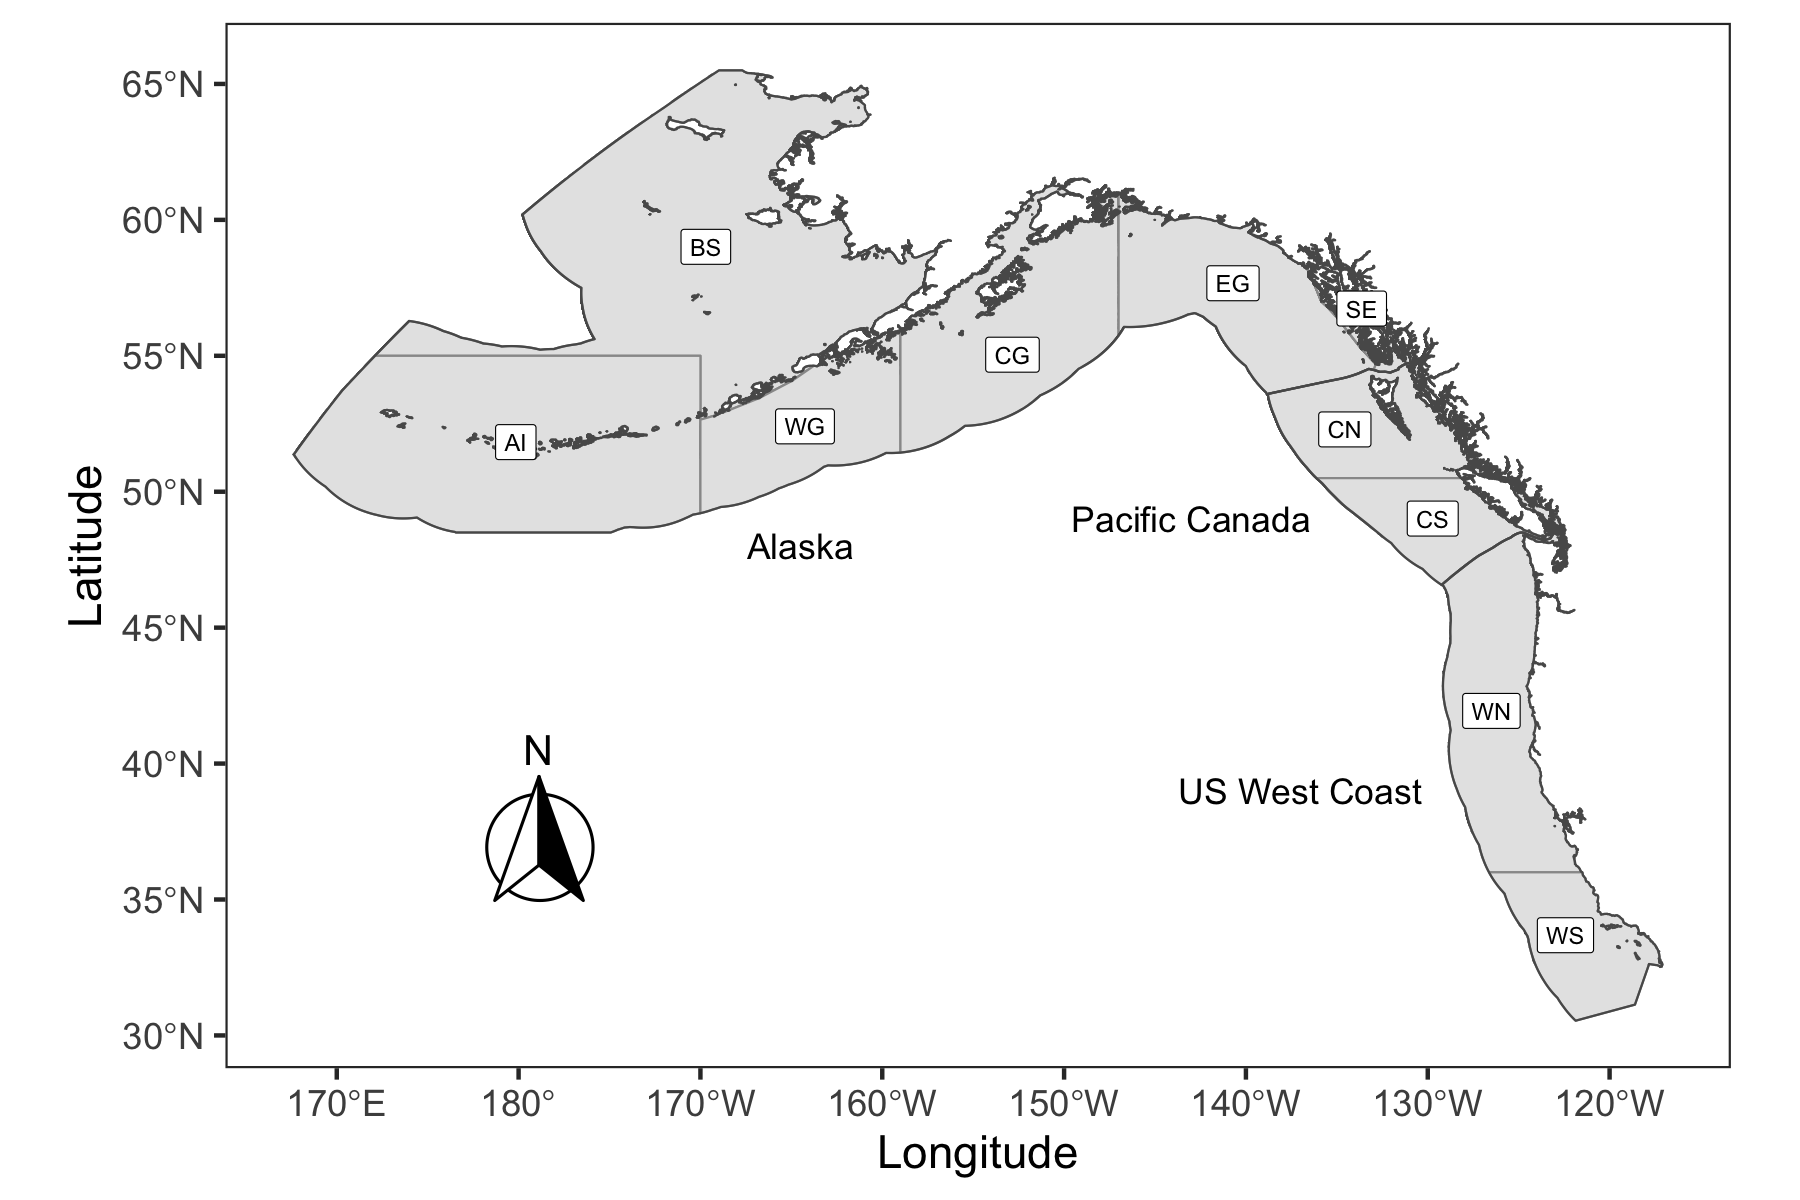
\includegraphics[width = \textwidth]{map-regions-areas}
    \caption{Sablefish release and recovery areas at two spatial scales in the northeast Pacific Ocean. Alaska, Pacific Canada and the US West Coast (black lines) were defined by their respective Exclusive Economic Zones (EEZ). Ten areas within the EEZs (grey lines) were the Bering Sea (BS), Aleutian Islands (AI), Western (WG), Central (CG), and Eastern Gulf of Alaska (EG), Southeast Alaska (SE), Pacific Canada North (CN), Pacific Canada South (CS), US West Coast North (WN), and US West Coast South (WS). \lr{TODO: Add inset showing NE Pacific in context; add land layer; emphasize difference between EEZ and small area boundaries}}
    \label{fig:map-regions-areas}
\end{figure}

% Heat movement 03a static
\begin{figure}[htb]
    \centering
    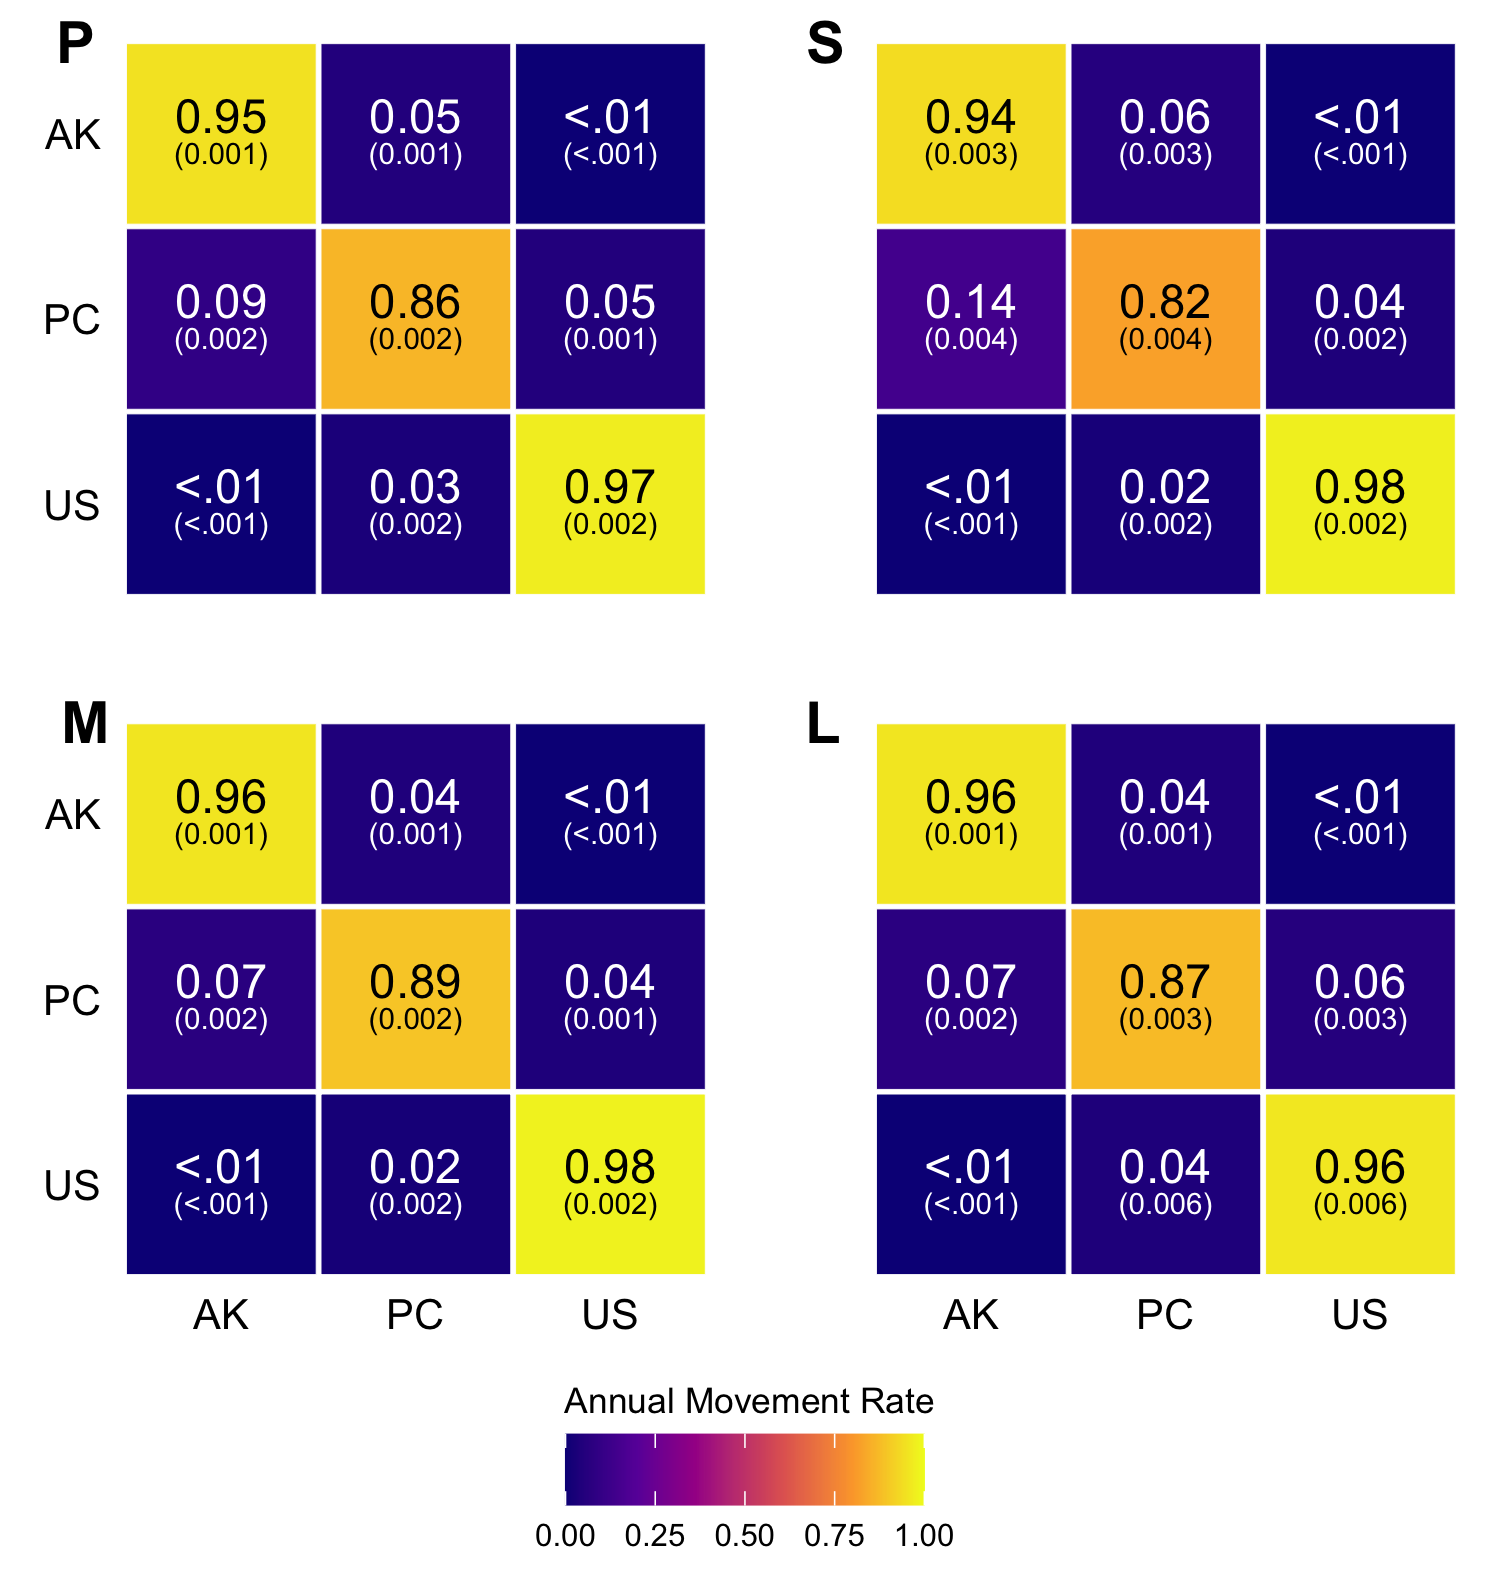
\includegraphics[width = 5in]{figs/heat-movement-03a-static}
    \caption{Annual movement rates among Alaska (AK), Pacific Canada (PC) and the US West Coast (US). Length classes are \textbf{P.} pooled, \textbf{S.} small, \textbf{M.} medium, and \textbf{L.} large. Rates (and standard errors) measure the probability that a sablefish from one area (row) moved to another area (column) in any given year.}
    \label{fig:heat-movement-03a-static}
\end{figure}

% Heat movement 10a static
\begin{figure}[htb]
    \centering
    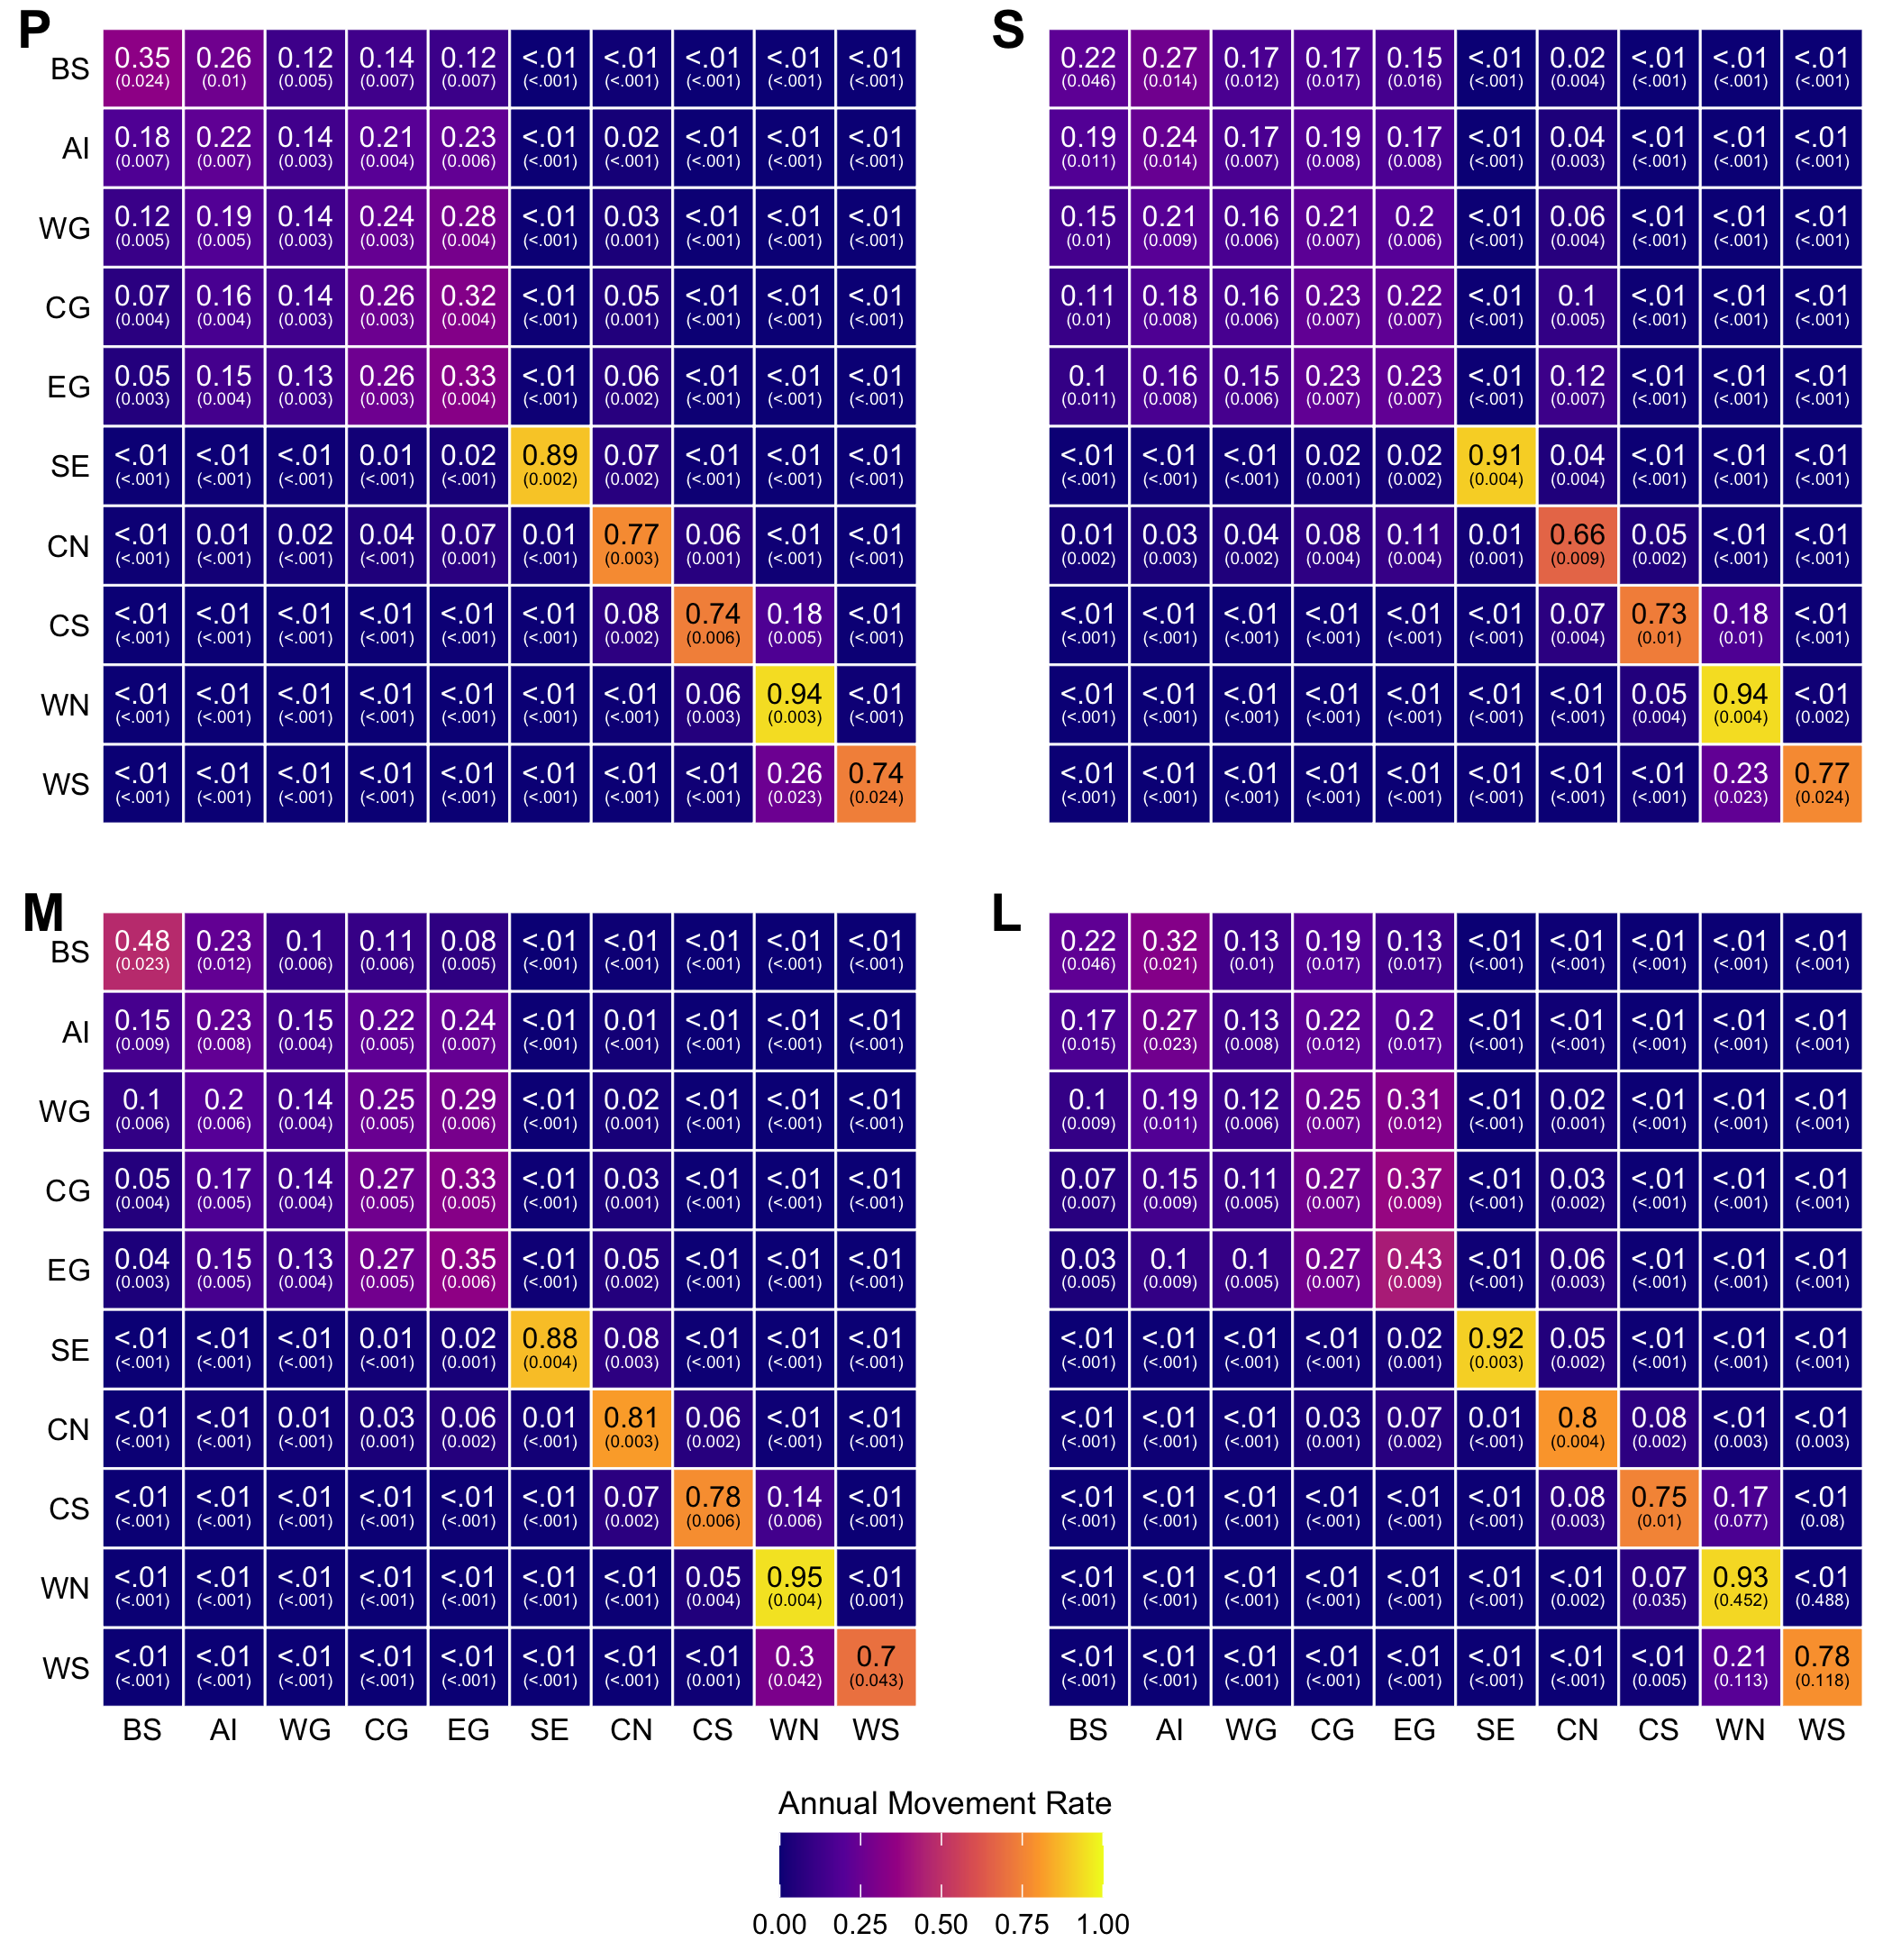
\includegraphics[width = \textwidth]{figs/heat-movement-10a-static}
    \caption{Annual movement rates among areas within Alaska, Pacific Canada and the US West Coast. Areas are Bering Sea (BS), Aleutian Islands (AI), Western Gulf (WG), Central Gulf (CG), Eastern Gulf (EG), Southeast Alaska (SE), Pacific Canada North (CN), Pacific Canada South (CS), US West Coast North (WN), and US West Coast South (WS). Length classes are \textbf{P.} pooled, \textbf{S.} small, \textbf{M.} medium, and \textbf{L.} large. Rates (and standard errors) measure the probability that a sablefish from one area (row) moved to another area (column) during one year.}
    \label{fig:heat-movement-10a-static}
\end{figure}

% Figure 4: AB: caption should say decadal, not annual, or time-block movement rates or similar…
% DG: West coast US fish do not move….
% KF: Consider referring to US West Coast as WC instead of US (here and elsewhere), it’s a bit more in line with other places that you use WS and WN to refer to west coast north and south. 
% LR: Something like Average annual movement rates for decadal time blocks

% Line movement 03a time varying
\begin{figure}[htb]
    \centering
    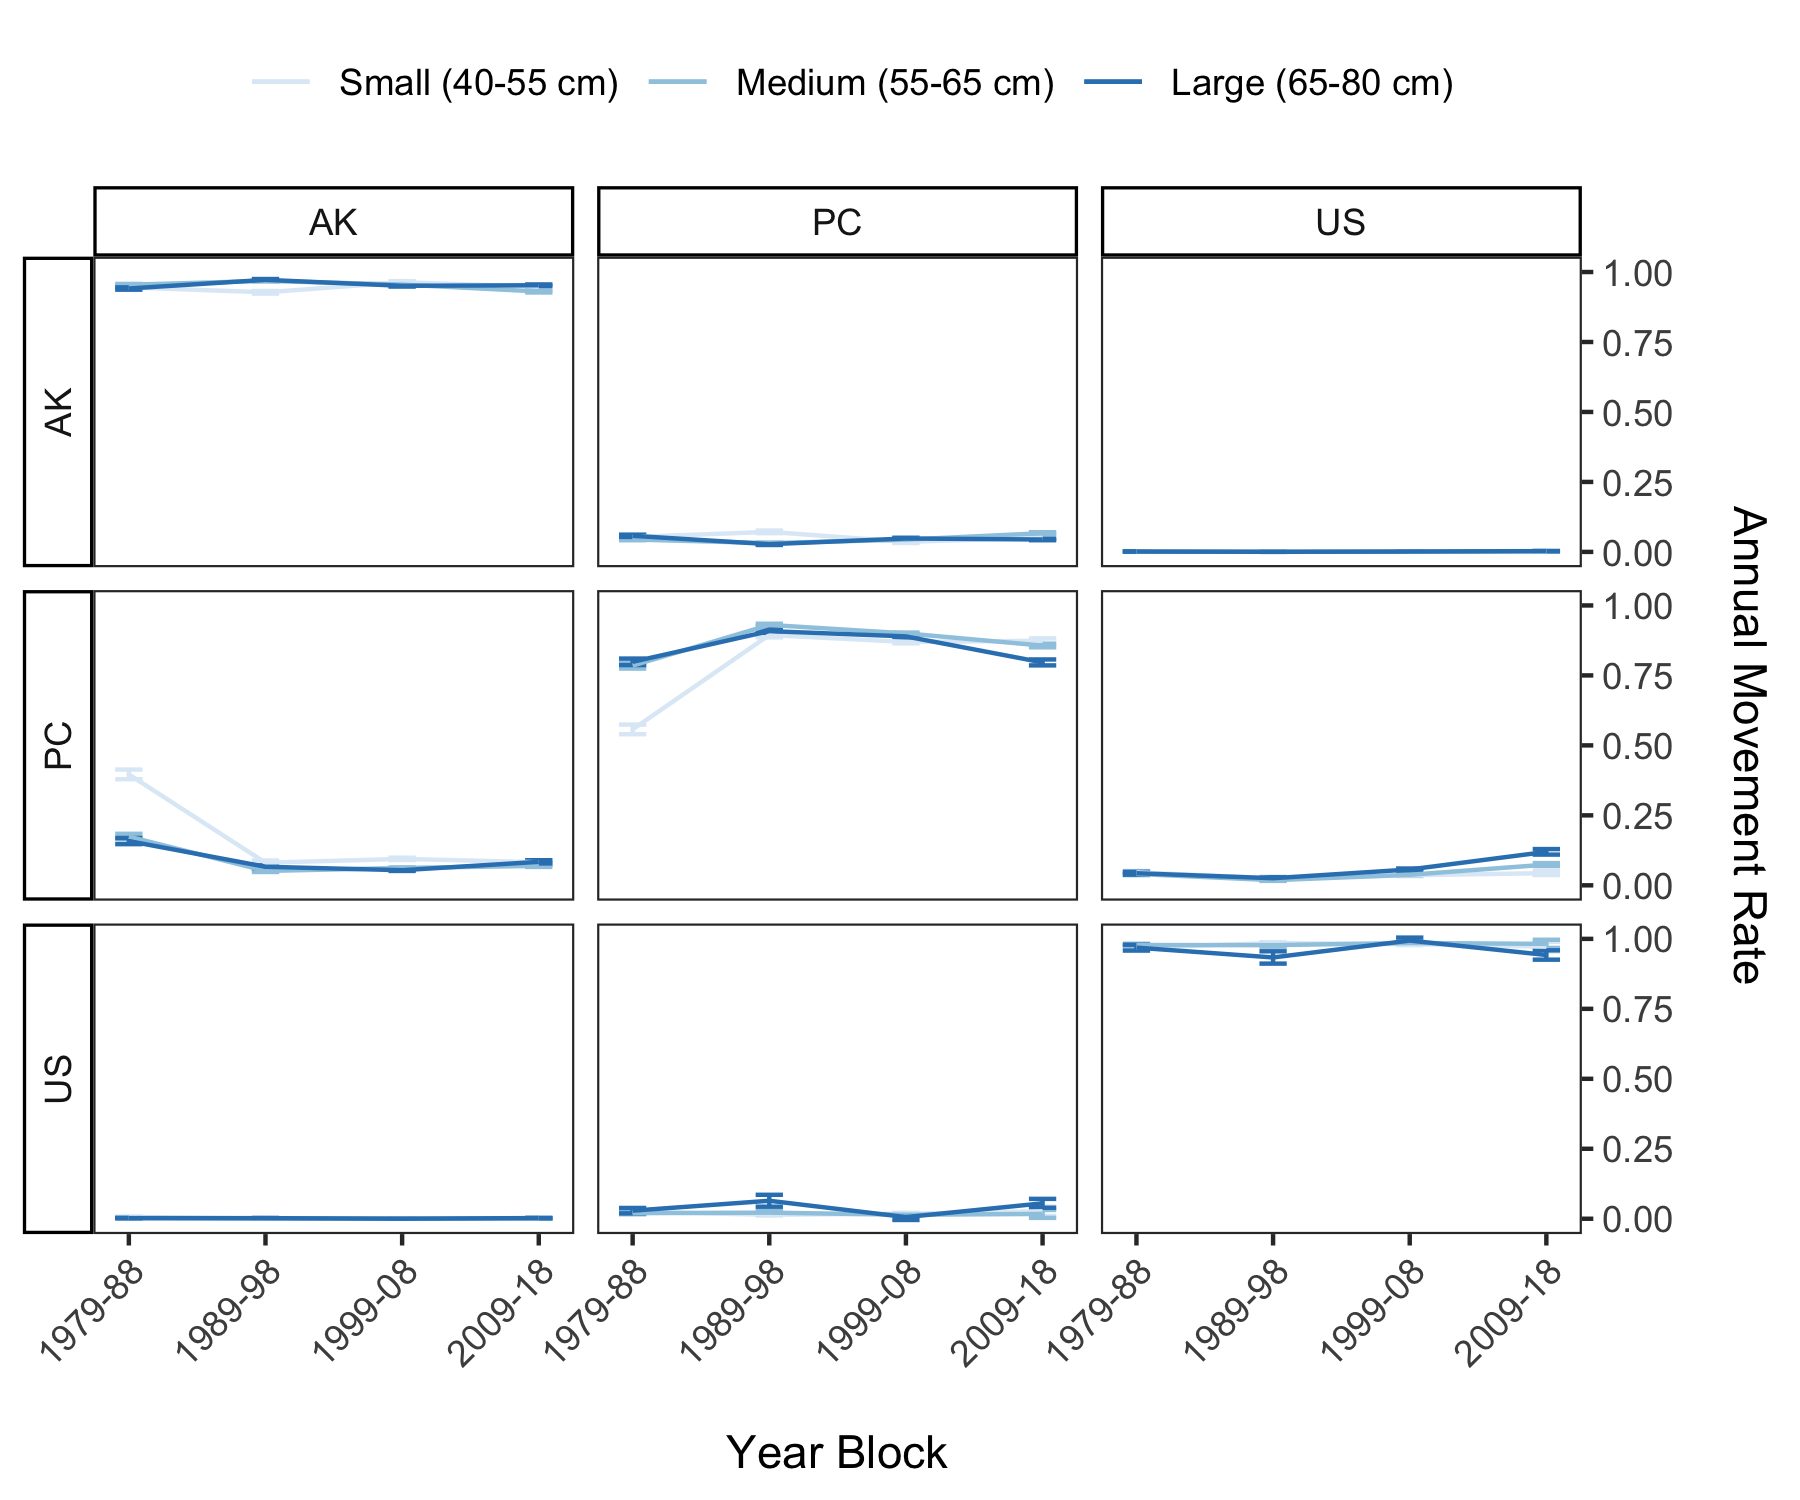
\includegraphics[width = \textwidth]{figs/line-movement-03a-size-sml-timevary}
    \caption{Annual movement rates among Alaska (AK), Pacific Canada (PC) and the US West Coast (US) estimated for ten year blocks. Length classes are small (lightest blue), medium (intermediate blue), and large (darkest blue). Error bars show one standard error. Movement rates measure the probability that a sablefish from one area (row) moved to another area (column) in any given year.}
    \label{fig:line-movement-03a-size-sml-timevary}
\end{figure}

% Figure 5: MH: Okay, now I see that these are millions of fish, I would add ‘of fish’ to the axis labels. It would also be interesting to see this converted to age X+ biomass or spawning biomass and this is the unit of management. 
% DG: Yea I was thinking it might be worth just providing a figure of emigration and immigration as a fraction of existing abundance in each area (e.g., # leaving AK/#in AK, #coming into AK/#In AK).

% Bar abundance exchange pool sml
\begin{figure}[htb]
    \centering
    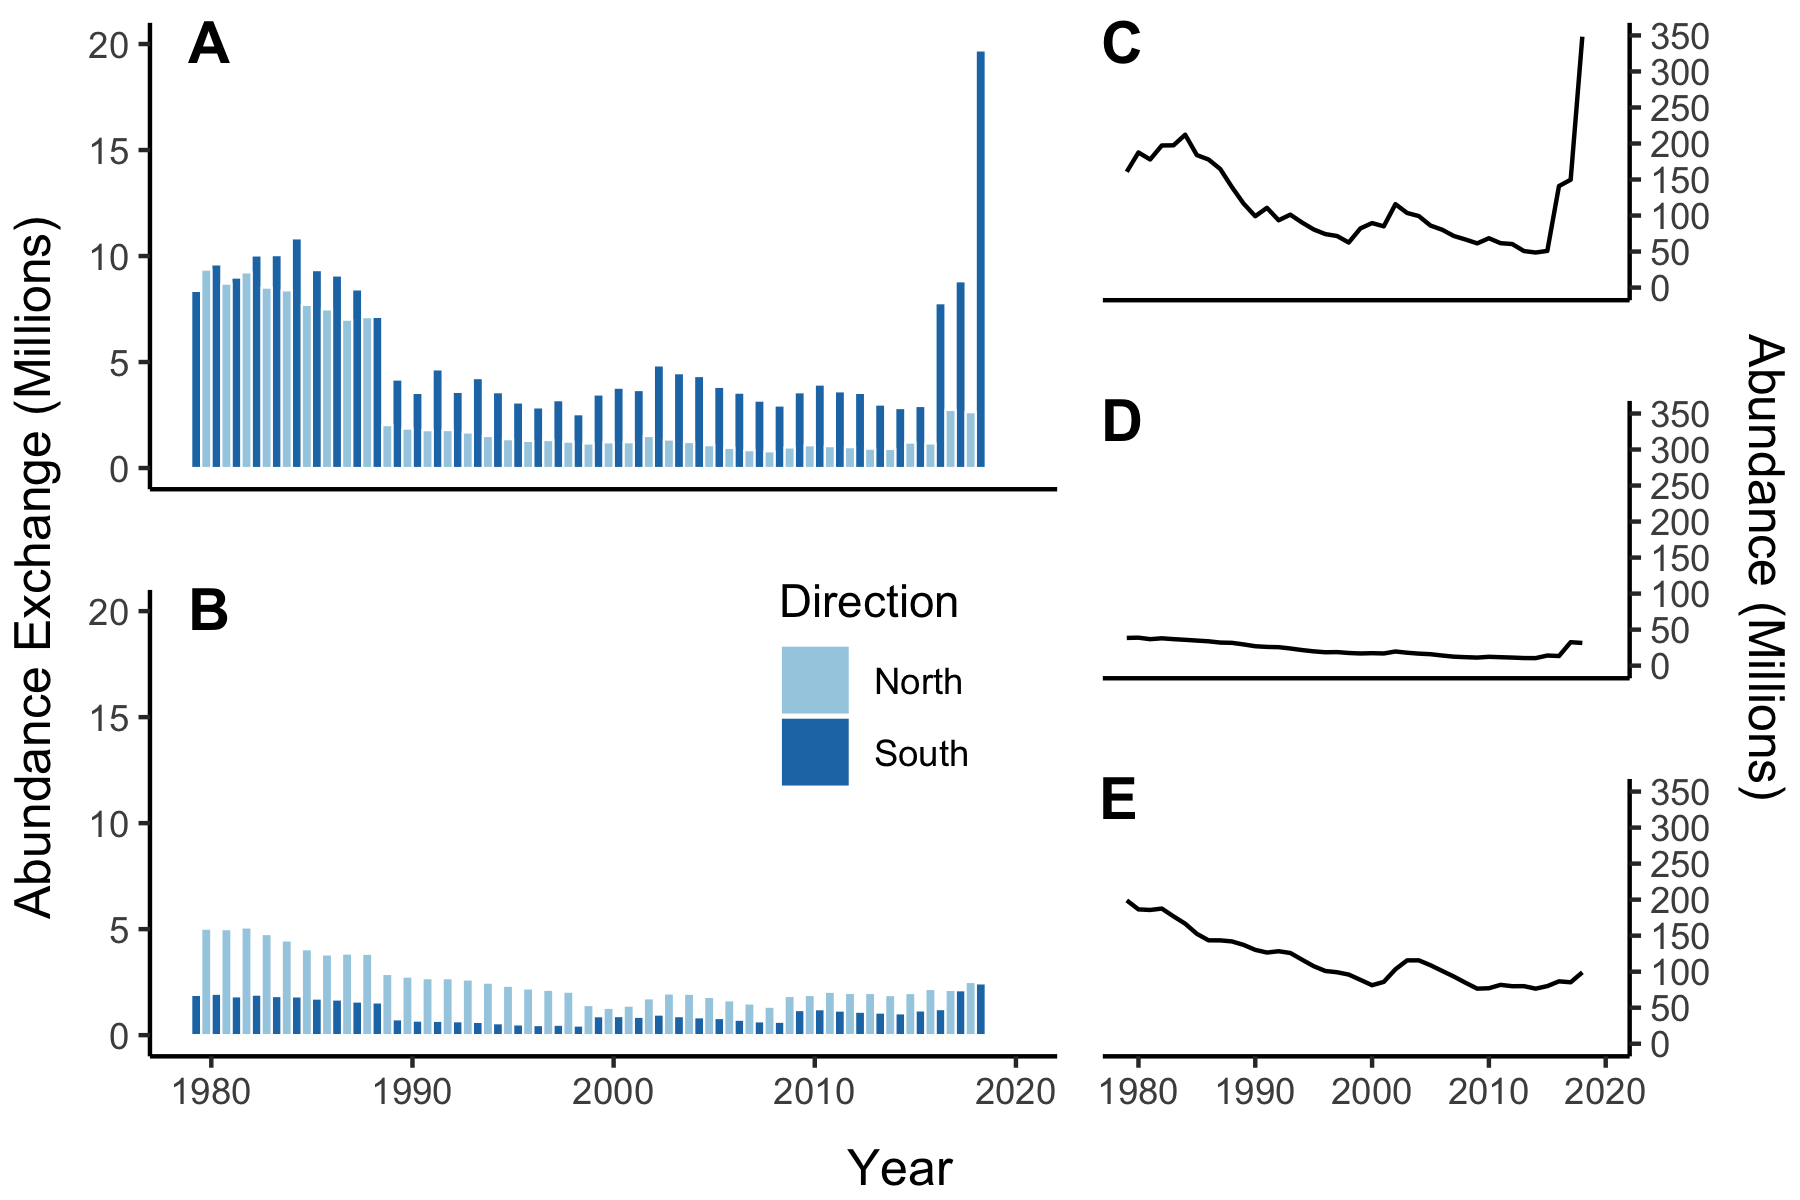
\includegraphics[width = \textwidth]{figs/bar-abundance-exchange-pool-sml}
    \caption{Sablefish abundance exchange between EEZs and abundance within EEZ. \textbf{A.} Alaska--Pacific Canada; \textbf{B.} Pacific Canada--US West Coast; \textbf{C.} Alaska; \textbf{D.} Pacific Canada; \textbf{E.} US West Coast. \lr{name lengths shown}}
    \label{fig:bar-abundance-exchange-pool-sml}
\end{figure}

% Map released recovered figure
\begin{figure}[htb]
    \centering
    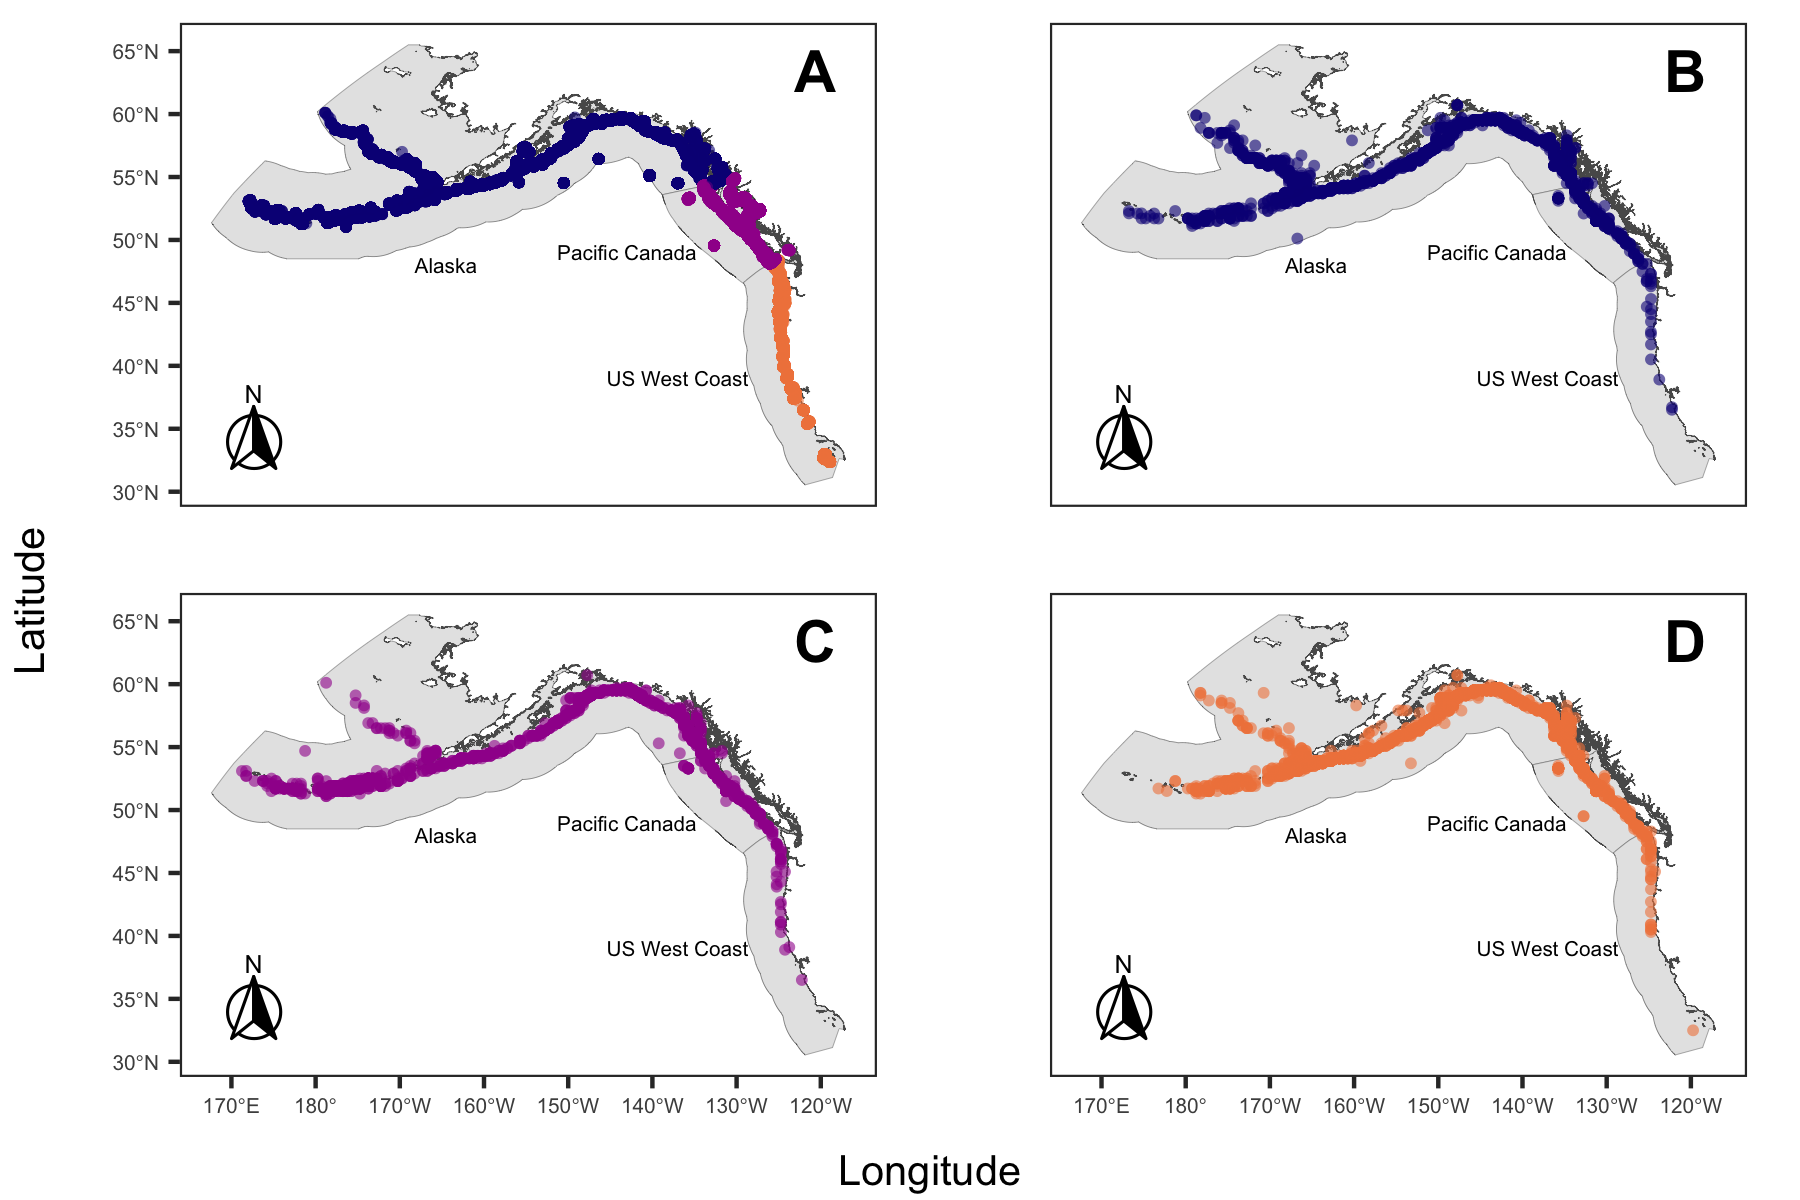
\includegraphics[width = \textwidth]{figs/map-released-recovered}
    \caption{\textbf{A.} Geographic extent of sablefish tag releases in Alaska, Pacific Canada, and the US West Coast. \textbf{B.--D.} Sablefish tag recoveries from releases in Alaska, Pacific Canada, and the US West Coast respectively. Tag release areas are Alaska (blue), Pacific Canada (purple), and the US West Coast (orange). \lr{TODO: Add land layer; check recovery maps meet anonymization standard}}
    \label{fig:map-released-recovered}
\end{figure}

% Bar annual releases by region
% \begin{figure}[htb]
%     \centering
%     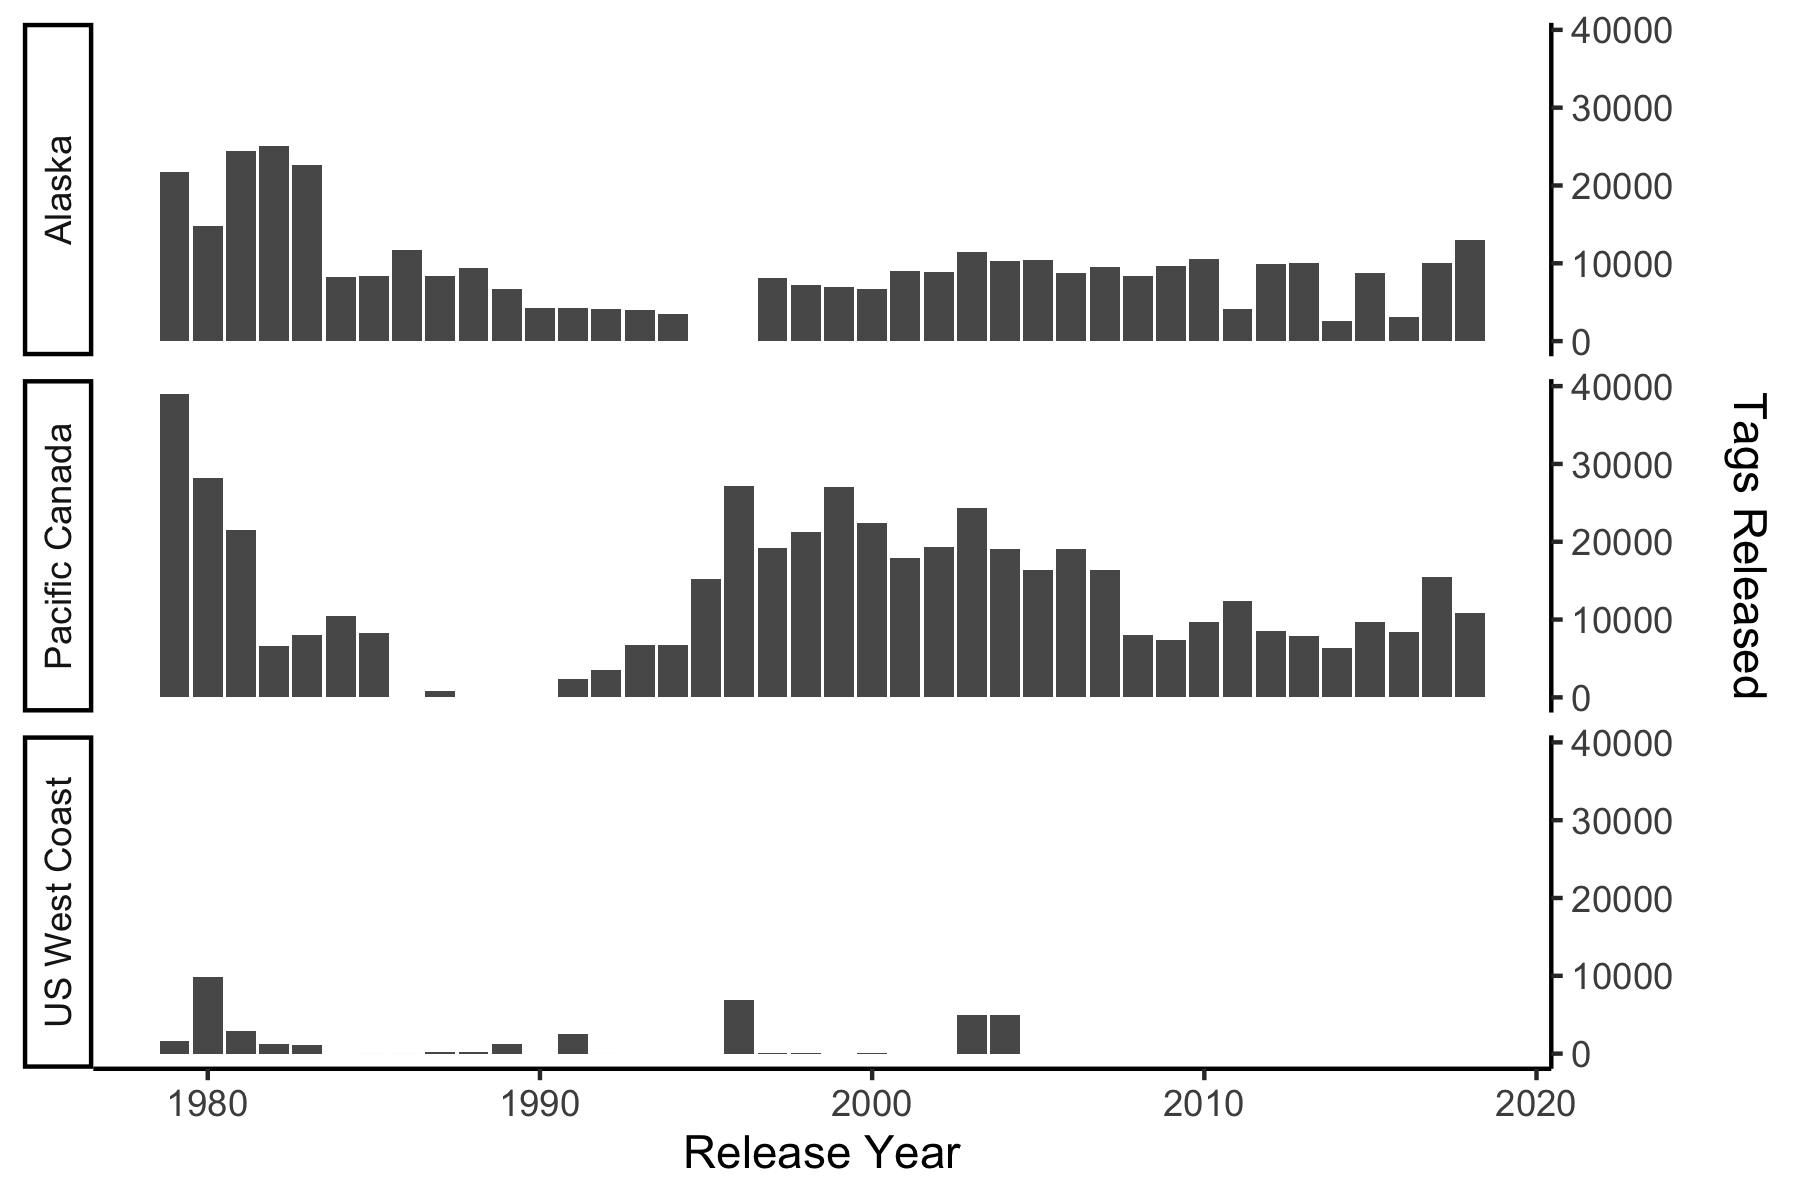
\includegraphics[width = \textwidth]{figs/bar-released-regions}
%     \caption{Annual sablefish tag releases from Alaska, Pacific Canada, and the US West Coast.}
%     \label{fig:bar-released-regions}
% \end{figure}

% Figure 7: AB: try to match figure with caption and main text in terms of mm or cm for length bins. The unused lengths are from not being mixed (i.e., recaptured the first time period) or…?  Grey doesn’t show behind/in front of the black.
% Figures 7-12: DG: I would suggest that these figures might be worth moving to Supplementary Material.
% KF - Figure 9...would be interesting to get feedback from Katy, others familiar with the tag data, about how realistic/accurate the tag recoveries data are by month for each EEZ. Is accuracy of tag return month crucial to the validity of the analyses? I am not sure what this figure adds to the story being told in the paper.

% Histogram of length by region
\begin{figure}[htb]
    \centering
    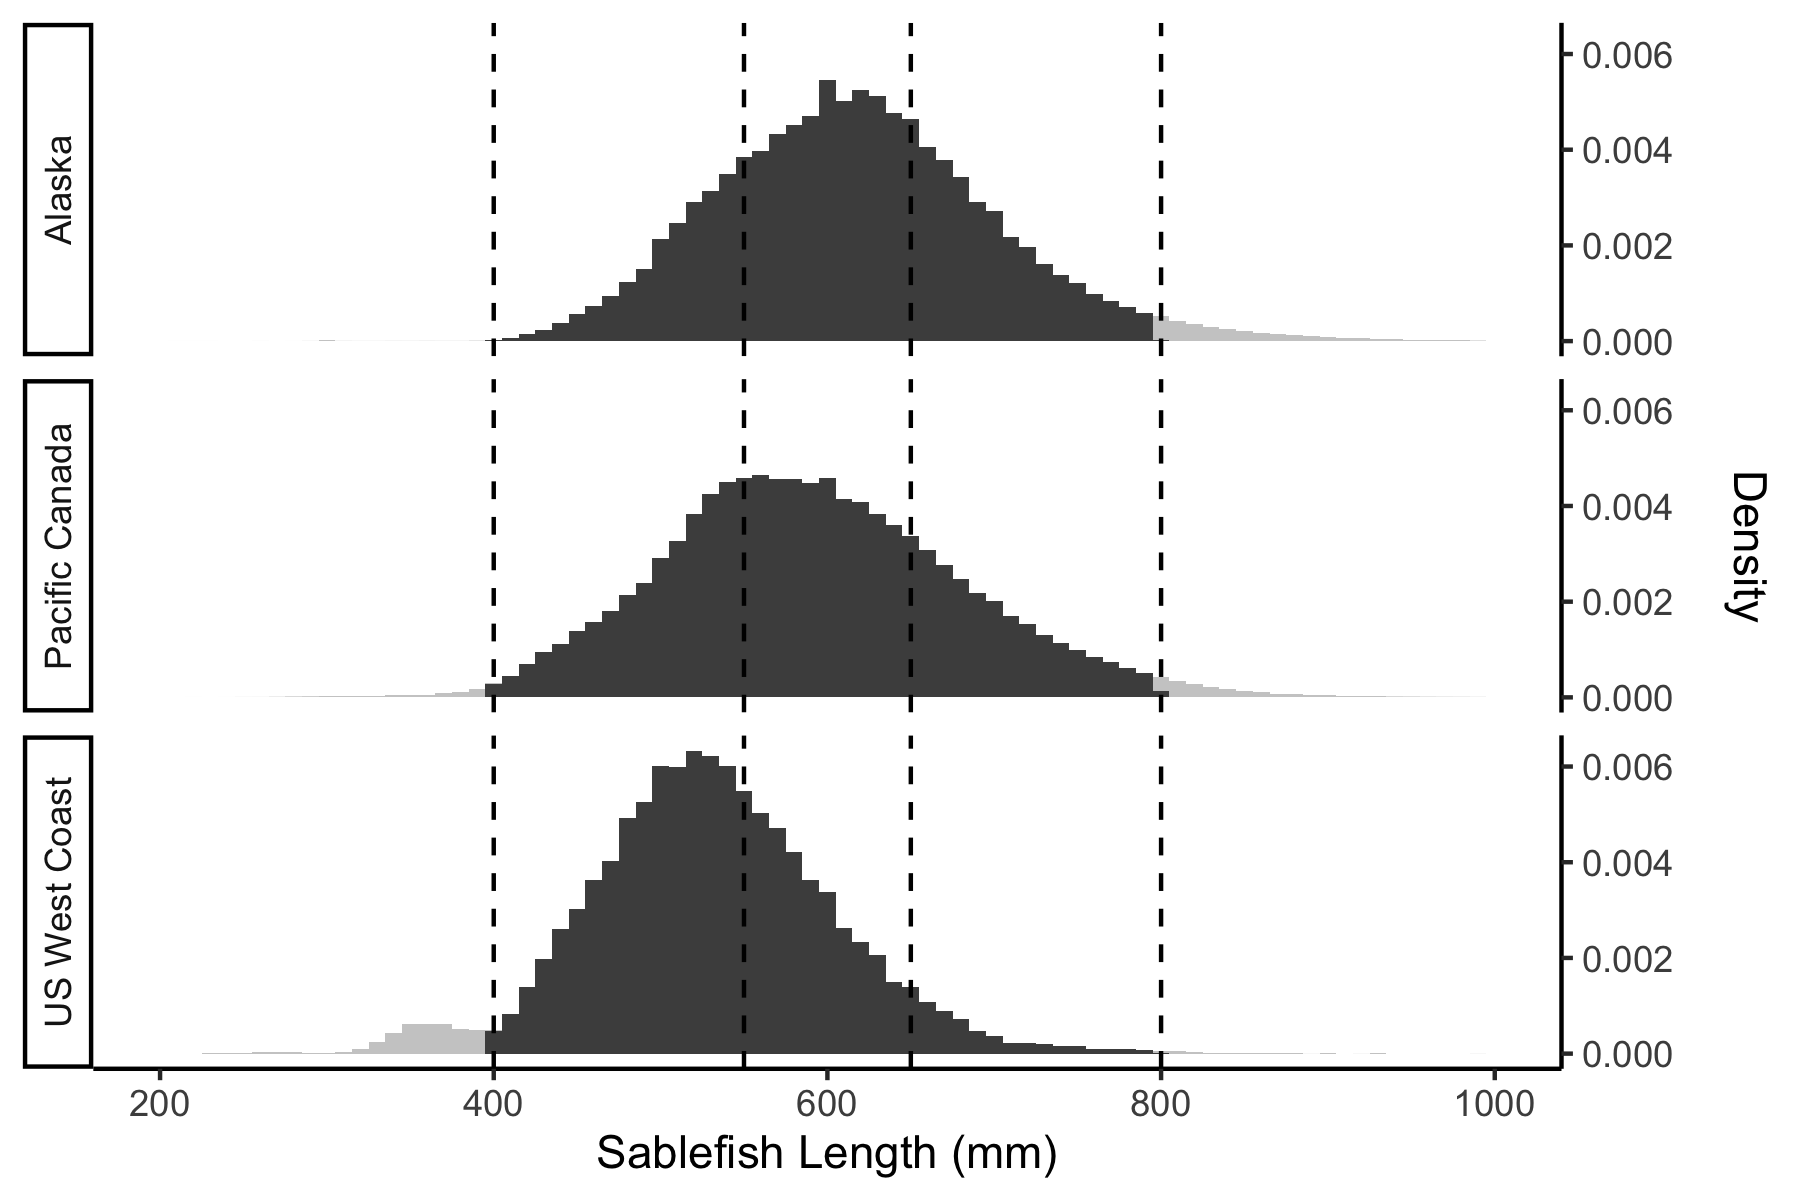
\includegraphics[width = \textwidth]{figs/hist-length-region}
    \caption{Length distributions of sablefish tag releases from Alaska, Pacific Canada and the US West Coast. Length classes are small (40--55 cm), medium (55--65 cm), and large (65--80 cm). The densities of unused lengths (light grey) are shown for comparison.}
    \label{fig:hist-length-region}
\end{figure}

% Line capture rate
\begin{figure}[htb]
    \centering
    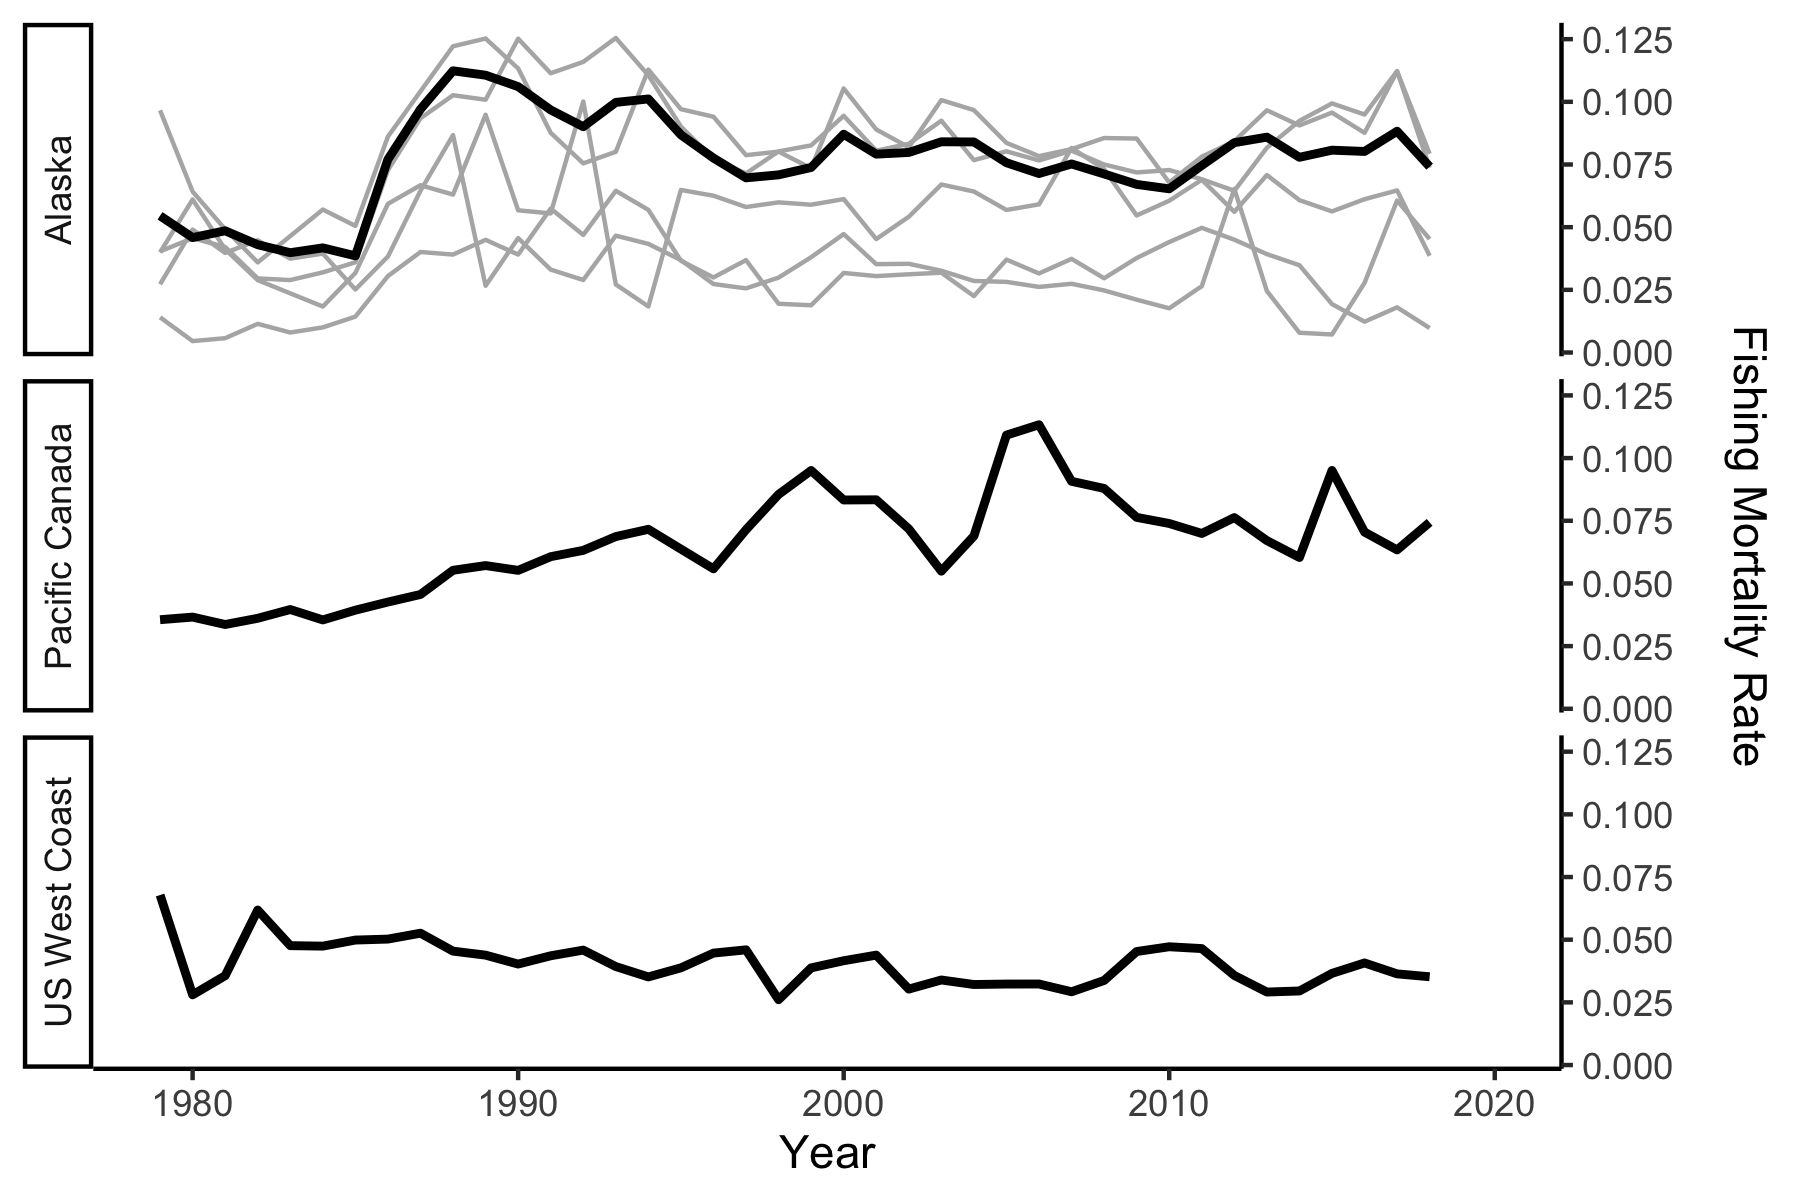
\includegraphics[width = \textwidth]{figs/line-capture-rate}
    \caption{Instantaneous annual fishing mortality rates for \textbf{A.} Alaska, \textbf{B.} Pacific Canada and \textbf{C.} the US West Coast. Rates are for EEZs (dark grey) or areas within EEZs (light grey).}
    \label{fig:line-capture-rate}
\end{figure}

% Bar capture scale region
\begin{figure}[htb]
    \centering
    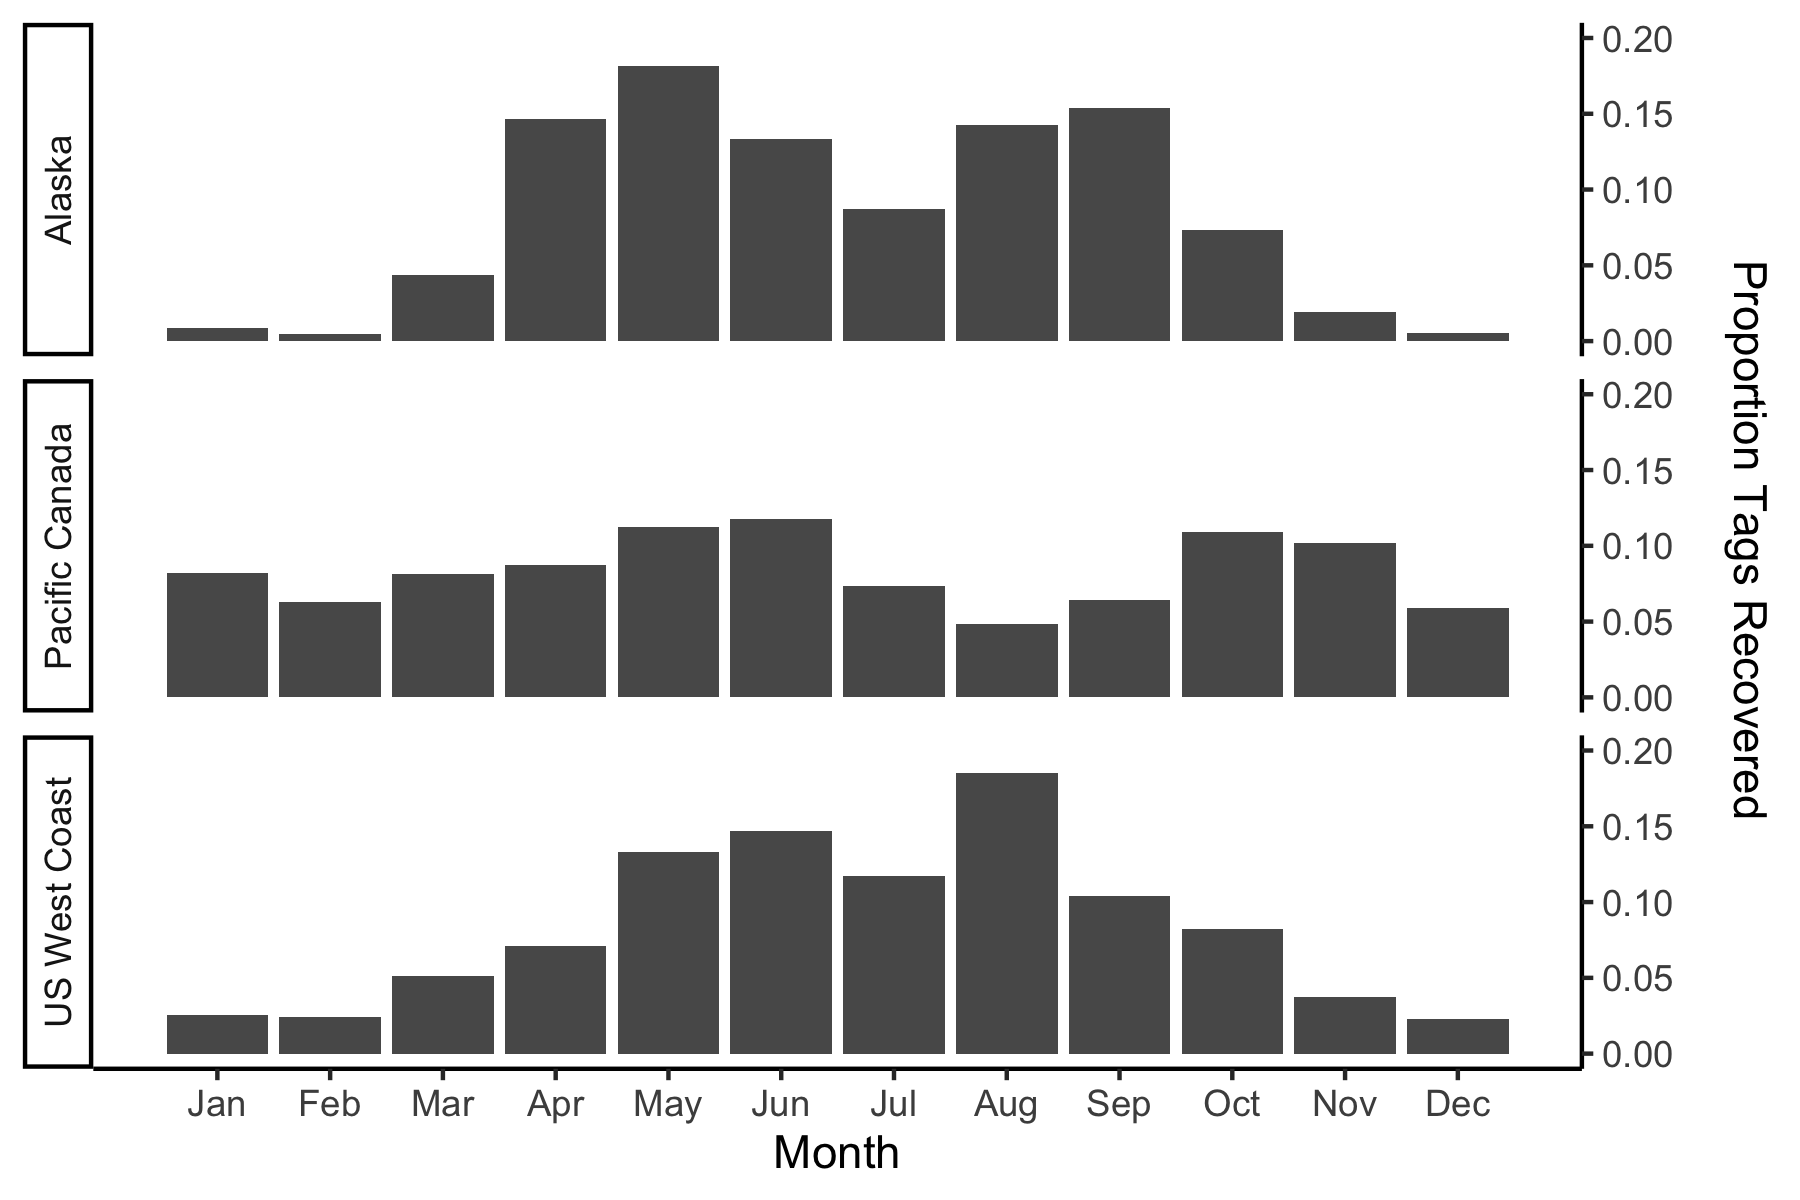
\includegraphics[width = \textwidth]{figs/bar-capture-scale-region}
    \caption{Distribution of sablefish tag recoveries by month for Alaska, Pacific Canada, and the US West Coast.}
    \label{fig:bar-capture-scale-region}
\end{figure}

% Bar capture scale area
\begin{figure}[htb]
    \centering
    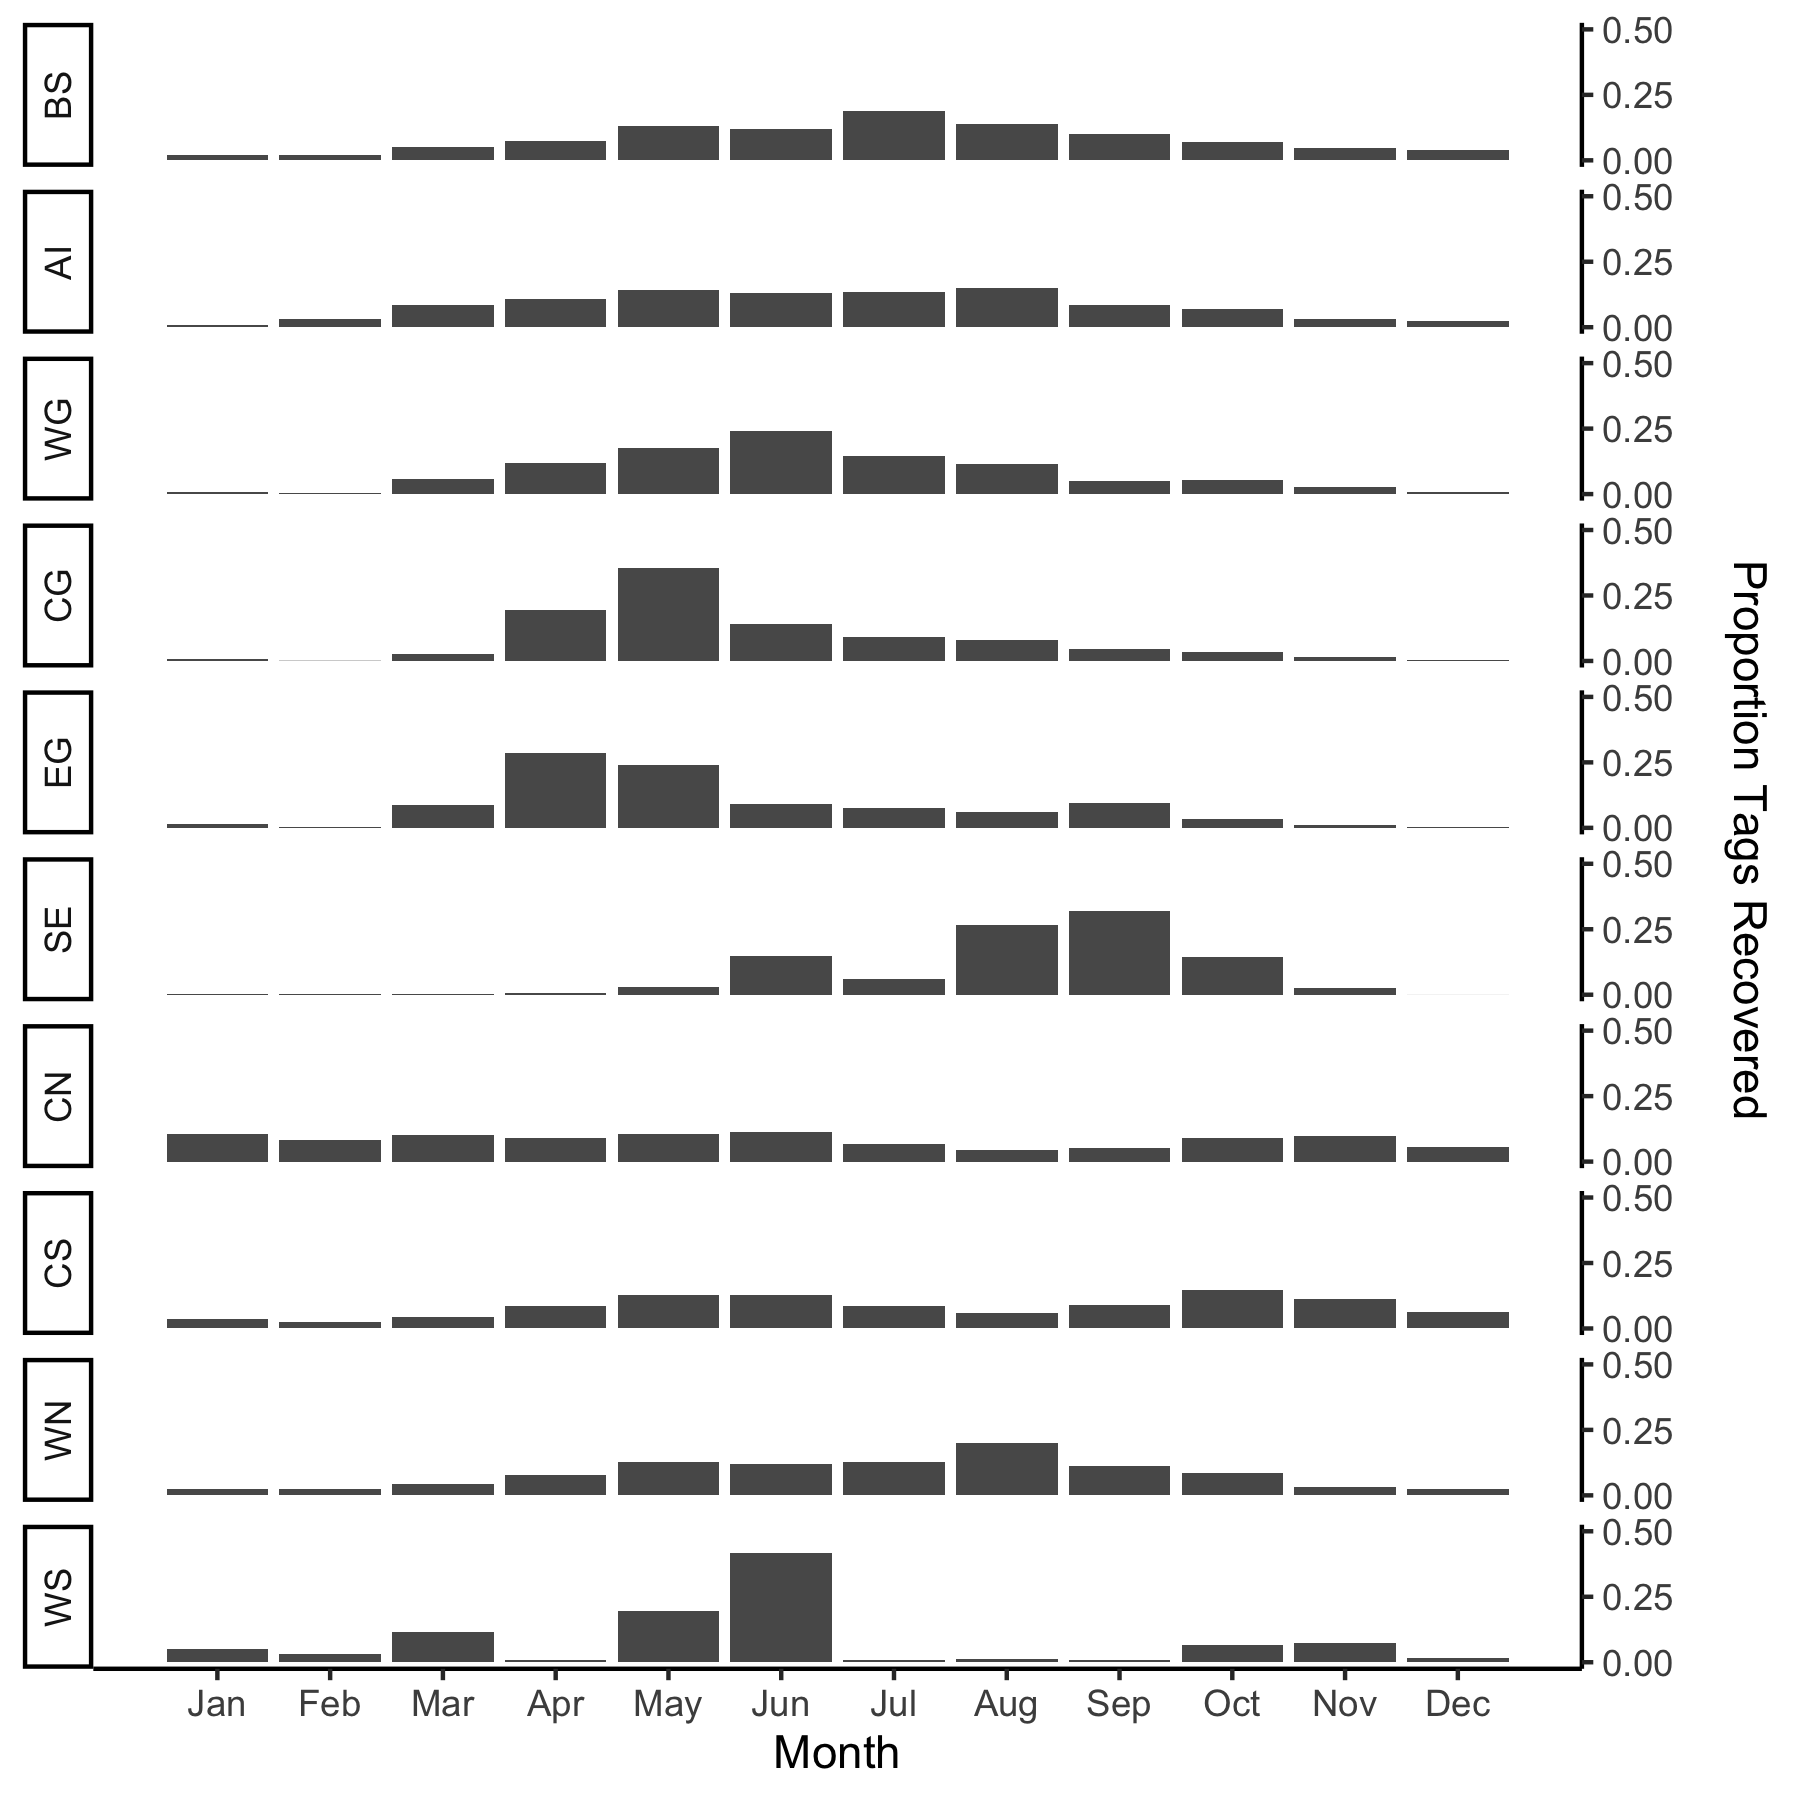
\includegraphics[width = \textwidth]{figs/bar-capture-scale-area}
    \caption{Distribution of sablefish tag recoveries by month for areas within Alaska, Pacific Canada, and the US West Coast. Areas are Bering Sea (BS), Aleutian Islands (AI), Western Gulf (WG), Central Gulf (CG), Eastern Gulf (EG), Southeast Alaska (SE), Pacific Canada North (CN), Pacific Canada South (CS), US West Coast North (WN), and US West Coast South (WS).}
    \label{fig:bar-capture-scale-area}
\end{figure}

% Line report rate
\begin{figure}[htb]
    \centering
    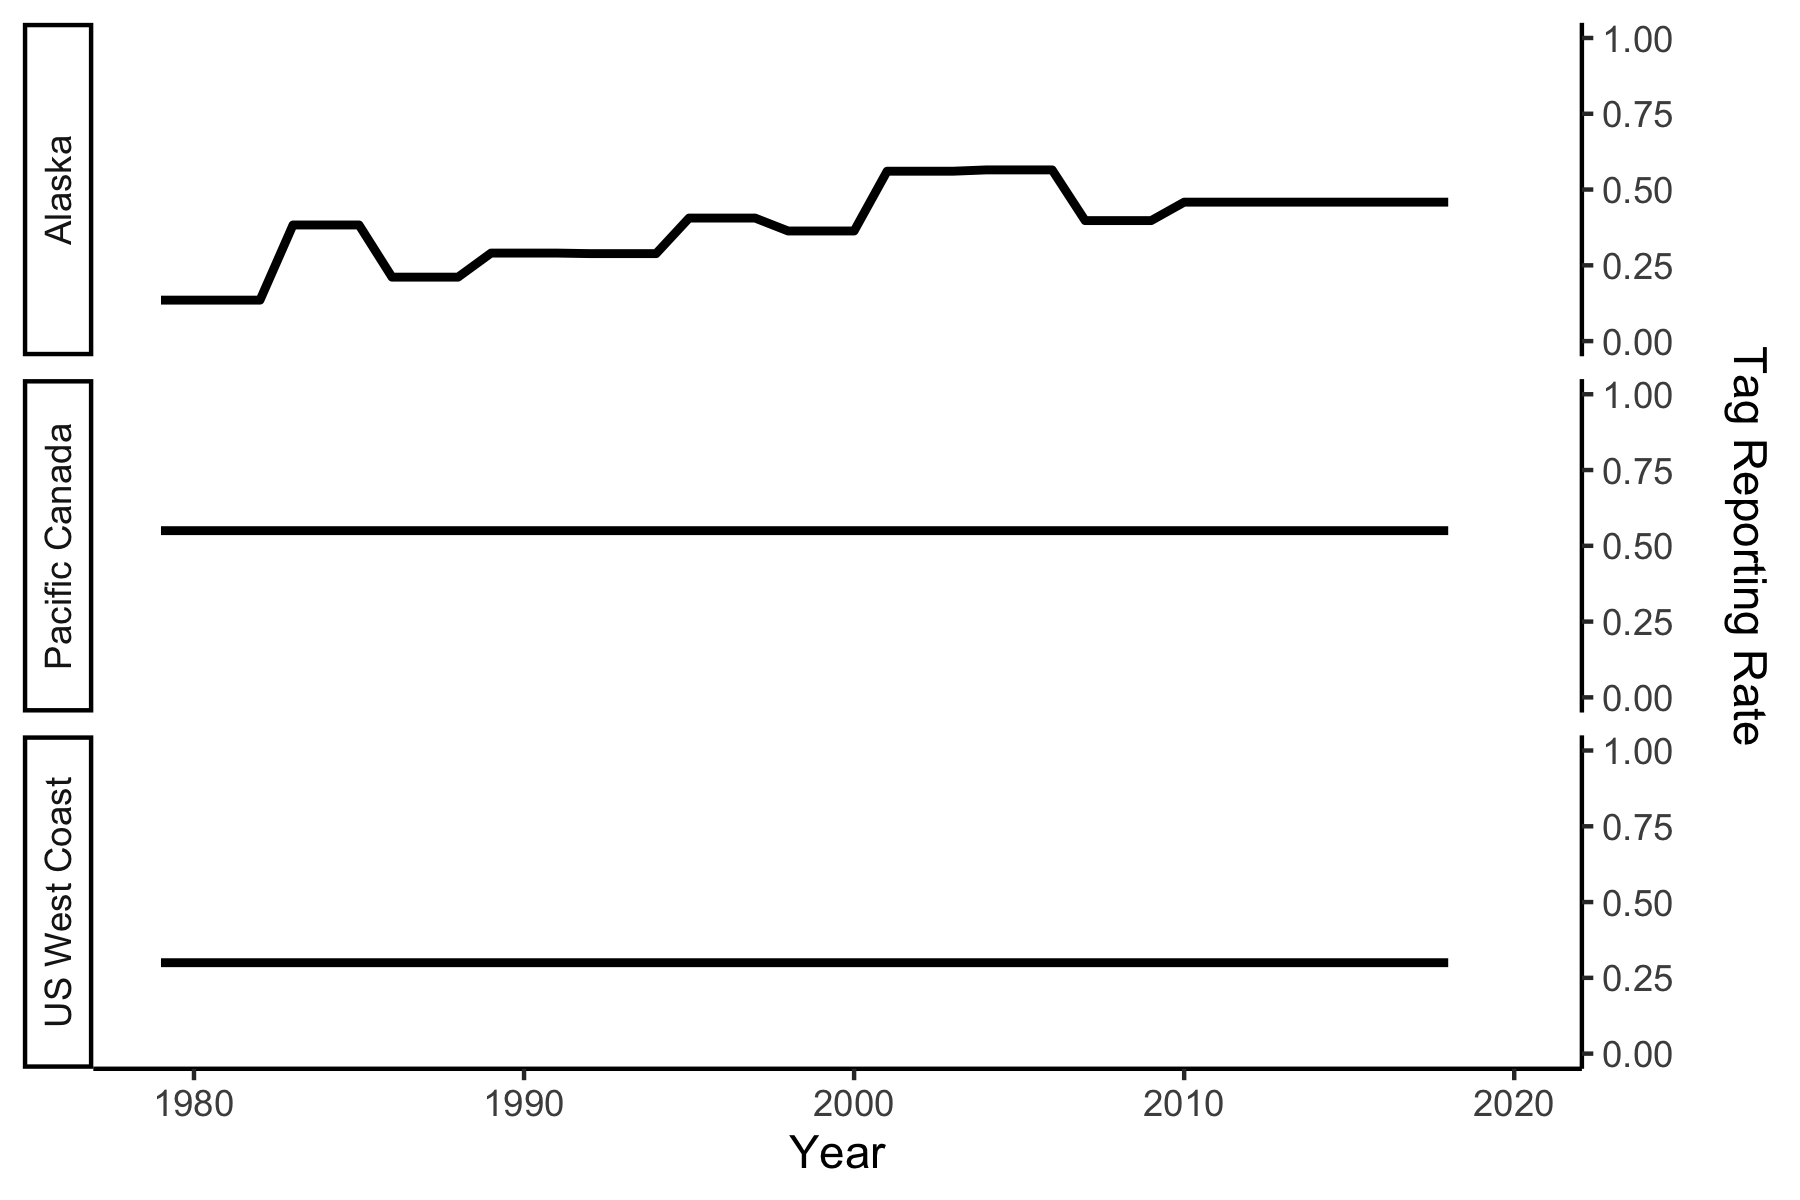
\includegraphics[width = \textwidth]{figs/line-report-ratio}
    \caption{Tag reporting rates for \textbf{A.} Alaska, \textbf{B.} Pacific Canada, and \textbf{C.} the US West Coast.}
    \label{fig:line-report-ratio}
\end{figure}

% Bar sensitivity
\begin{figure}[htb]
    \centering
    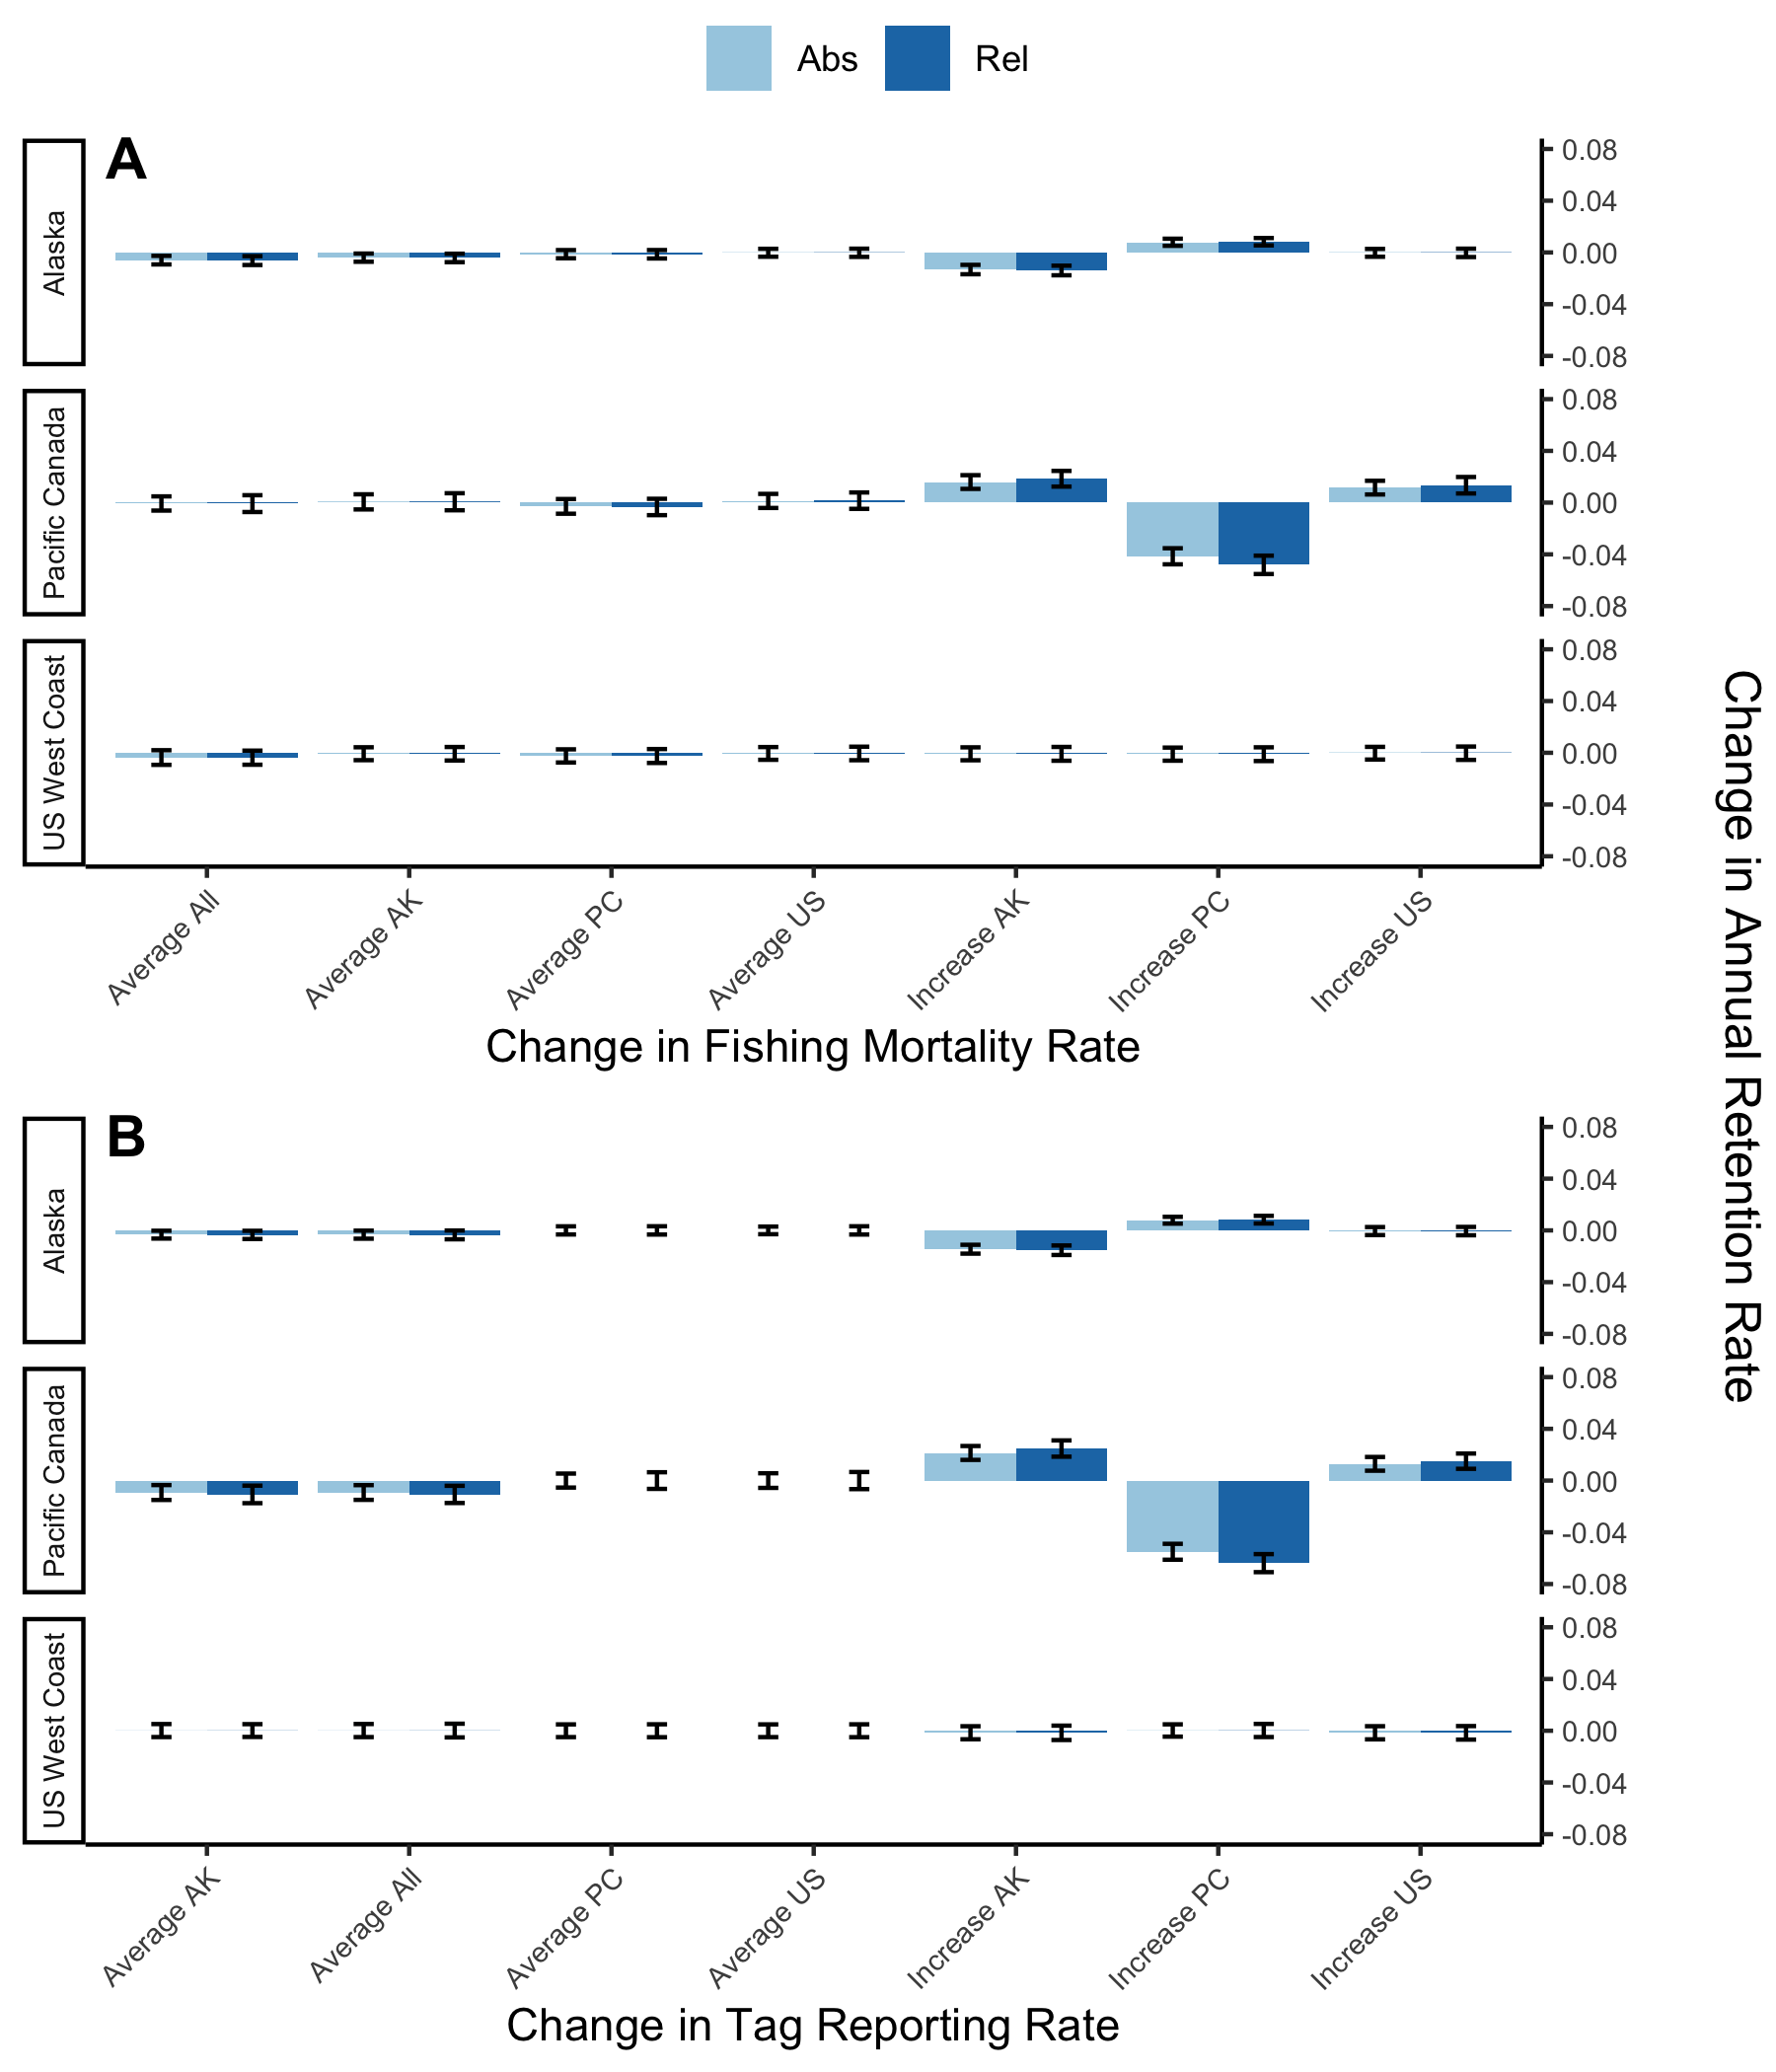
\includegraphics[width = \textwidth]{figs/bar-sensitivity}
    \caption{Sensitivity of retention rates to changes in \textbf{A.} fishing mortality rates and \textbf{B.} tag reporting rates. Average: yearly input replaced by its mean. Increase: yearly input increased by 50\%. Changes are absolute (light blue) or relative to the reference value (dark blue).}
    \label{fig:bar-sensitivity}
\end{figure}


\end{document}
